% ta med damping på DP-delle

\documentclass[aspectratio=169,xcolor=dvipsnames]{beamer}
%\usetheme{SimplePlus}

\usepackage{hyperref}
\usepackage{graphicx} % Allows including images
\usepackage{booktabs} % Allows the use of \toprule, \midrule and \bottomrule in tables

%----------------------------------------------------------------------------------------
%	TITLE PAGE
%----------------------------------------------------------------------------------------

\title[Trykk]{Målesystemer for trykk} % The short title appears at the bottom of every slide, the full title is only on the title page
%\subtitle{Subtitle}

\author[Fred-Olav] {Fred-Olav Mosdal}

\institute[Gand VGS] % Your institution as it will appear on the bottom of every slide, may be shorthand to save space
{
    Gand VGS \\
    VG3 Automasjon
}
\date{\today} % Date, can be changed to a custom date


%----------------------------------------------------------------------------------------
%	PRESENTATION SLIDES
%----------------------------------------------------------------------------------------

\begin{document}
%\section{Cascade control}
%
%A simple control system drawn in block diagram form looks like this:
%
\begin{frame}
\titlepage
\end{frame}
%A \textit{fluid} is any substance having the ability to \textit{flow}: to freely change shape and move under the influence of a motivating force.  Fluid motion may be analyzed on a microscopic level, treating each fluid molecule as an individual projectile body.  This approach is extraordinarily tedious on a practical level, but still useful as a model of fluid behavior.  \index{Fluid}
%
%Some fluid properties are accurately predicted by this model, especially predictions dealing with potential and kinetic energies.  However, the ability of a fluid's molecules to independently move give it unique properties that solids do not possess.  One of these properties is the ability to effortlessly transfer \textit{pressure}, defined as force applied over area. \index{Pressure}





%\filbreak
%\subsection{Pressure}
%
%The common phases of matter are \textit{solid}, \textit{liquid}, and \textit{gas}.  Liquids and gases are fundamentally distinct from solids in their intrinsic inability to maintain a fixed shape.  In other words, liquids and gases tend to fill whatever solid containers they are held in.  Similarly, both liquids and gases both have the ability to flow, which is why they are collectively called \textit{fluids}. \index{Solid}  \index{Liquid}  \index{Gas} \index{Fluid}
%
%Due to their lack of definite shape, fluids tend to disperse any force applied to them.  This stands in marked contrast to solids, which tend to transfer force only in the applied direction.  Take for example the force transferred by a nail, from a hammer to a piece of wood:
%
%$$\includegraphics{pressure01.eps}$$
\begin{frame}
	\frametitle{Trykk}

	$$\includegraphics[height=7cm]{pressure01.eps}$$
\end{frame}

\begin{frame}
	\frametitle{Absolutt trykk, relativt trykk og differansetrykk}
Denne slide må lages
\end{frame}
%
%The impact of the hammer's blow is directed straight through the solid nail into the wood below -- nothing surprising here.
%
%\filbreak
%
%Now consider what a \textit{fluid} would do when subjected to the same hammer blow:
%
%$$\includegraphics{pressure02.eps}$$
\begin{frame}
	\frametitle{Trykk}

	$$\includegraphics[height=6cm]{pressure02.eps}$$
$$P = {F \over A}$$
\end{frame}
%
%Given the freedom of a fluid's molecules to move about, the impact of the hammer blow becomes directed \textit{everywhere} against the inside surface of the container (the cylinder).  This is true for all fluids: liquids and gases alike.  The only difference between the behavior of a liquid versus a gas in the same scenario is that the gas will compress (i.e. the piston will move down as the hammer struck it), whereas the liquid will not compress (i.e. the piston will remain in its resting position).  Gases yield under pressure, liquids do not.
%
%It is very useful to quantify force applied to a fluid in terms of force per unit area, since the force applied to a fluid becomes evenly dispersed in all directions to the surface containing it.  This is the definition of \textit{pressure}\footnote{The concept of pressure is also applicable to solid materials: applying either a compressive or tensile force to a solid object of given cross-sectional area generates a \textit{pressure} within that object, also referred to as \textit{stress}.} ($P$): the amount of force ($F$) distributed across a given area ($A$). \index{Pressure}  \index{Stress}
%
%$$P = {F \over A}$$
%
%In the metric system, the standard unit of pressure is the \textit{pascal} (Pa), defined as one Newton (N) of force per square meter (m$^{2}$) of area.  In the British system of measurement, the standard unit of pressure is the \textit{PSI}: pounds (lb) of force per square inch (in$^{2}$) of area.  Pressure is often expressed in units of kilopascals (kPa) when metric units are used because one pascal is a rather small\footnote{To give some perspective on this, 1 pascal of pressure is equal to (only) 0.000145 pounds per square inch!} pressure for most engineering applications.  \index{Pascal, pressure unit}  \index{PSI}  \index{Pound per square inch, pressure unit}
%
%\filbreak
%
%The even distribution of force throughout a fluid has some very practical applications.  One application of this principle is the \textit{hydraulic lift}, which functions somewhat like a fluid lever: \index{Hydraulic lift}
%
%$$\includegraphics{pressure03.eps}%$$
\begin{frame}
	\frametitle{Pascal prinsipp}

	$$\includegraphics[height=6cm]{pressure03.eps}$$
\end{frame}
%
%Force applied to the small piston creates a pressure throughout the fluid.  That pressure exerts a greater force on the large piston than what is exerted on the small piston, by a factor equal to the ratio of piston areas.  Since area for a circular piston is proportional to the square of the radius ($A = \pi r^2$), even modest ratios of piston diameter yield large ratios of area and therefore of force.  If the large piston has five times the area of the small piston (i.e. the large piston's diameter is 2.236 times greater than the small piston's diameter), force will be multiplied five-fold.  Just as with the lever, however, there must be a trade-off so as to not violate the Conservation of Energy.  The trade-off for increased force is decreased distance, whether in the lever system or in the hydraulic lift system.  If the large piston generates a force five times greater than what is applied to the small piston, it must move only one-fifth as far as the small piston's motion.  In this way, energy in equals energy out (remember that \textit{work}, which is equivalent to energy, is calculated by multiplying force by parallel distance traveled).  \index{Conservation of Energy}
%
%\filbreak
%
%For those familiar with electricity, what you see here in either the lever system or the hydraulic lift is analogous to a \textit{transformer}: we can step AC voltage up, but only by reducing AC current.  Being a passive device, a transformer cannot boost power.  Therefore, power out can never be greater than power in, and given a perfectly efficient transformer, power out will always be precisely equal to power in:
%
%$$\hbox{Power} = (\hbox{Voltage in}) (\hbox{Current in}) = (\hbox{Voltage out}) (\hbox{Current out})$$
%
%$$\hbox{Work} = (\hbox{Force in}) (\hbox{Distance in}) = (\hbox{Force out}) (\hbox{Distance out})$$
%
%Fluid may be used to transfer power just as electricity is used to transfer power.  Such systems are called \textit{hydraulic} if the fluid is a liquid (usually oil), and \textit{pneumatic} if the fluid is a gas (usually air).  In either case, a machine (pump or compressor) is used to generate a continuous fluid pressure, pipes are used to transfer the pressurized fluid to the point of use, and then the fluid is allowed to exert a force against a piston or a set of pistons to do mechanical work: \index{Hydraulic} \index{Pneumatic}
%
%$$\includegraphics{pressure04.eps}$$
%
\begin{frame}
	\frametitle{Trykk}

	$$\includegraphics[height=6cm]{pressure04.eps}$$
\end{frame}
%To learn more about fluid power systems, refer to section \ref{Fluid power systems} beginning on page \pageref{Fluid power systems}.
%
%\filbreak
%
%An interesting use of fluid we see in the field of instrumentation is as a \textit{signaling medium}, to transfer information between places rather than to transfer power between places.  This is analogous to using electricity to transmit voice signals in telephone systems, or digital data between computers along copper wire.  Here, fluid pressure represents some other quantity, and the principle of force being distributed equally throughout the fluid is exploited to transmit that representation to some distant location, through piping or tubing:
%
%%$$\includegraphics{pressure05.eps}$$
\begin{frame}
	\frametitle{Trykk}

	$$\includegraphics[width=1\textwidth]{pressure05.eps}$$
\end{frame}
%
%This illustration shows a simple temperature-measuring system called a \textit{filled bulb}, where an enclosed bulb filled with fluid is exposed to a temperature that we wish to measure.  A rise in temperature makes the fluid expand and thereby increases pressure sensed at the gauge.  The purpose of the fluid here is two-fold: first to sense temperature, and second to relay this temperature measurement a long distance away to the gauge.  The principle of even pressure distribution allows the fluid to act as a signal medium to convey the information (bulb temperature) to a distant location. \index{Filled bulb}
%
%
%
%
%
%
%
%
%
%
%\filbreak
%\subsection{Pascal's Principle and hydrostatic pressure}
%
%\label{Physics of hydrostatic pressure}
%
%We learned earlier that fluids tend to evenly distribute any applied force.  This fundamental principle is the basis of fluid power and fluid signaling systems, where pressure is assumed to be transferred equally to all points in a confined fluid.  In the example of a hydraulic lift given earlier, we assume that the pressure throughout the fluid pathway is equal:
%
%$$\includegraphics{pressure15.eps}$$
\begin{frame}
	\frametitle{Pascals prinsipp og hydrostatisk trykk}

	$$\includegraphics[height=6cm]{pressure15.eps}$$
\end{frame}
%
%If additional force is applied to the small piston (say, 160 lbs instead of 150 lbs), the fluid pressure throughout the system will increase, not just the fluid pressure in the vicinity of the piston.  The effect of this additional force will be immediately\footnote{There is actually a speed of propagation to this increase in pressure, and it is the \textit{speed of sound} within that particular fluid.  This makes sense, since sound waves are nothing more than rapidly-changing regions of pressure within a material.} ``felt'' at all points of the system.  The phenomenon of pressure changes being evenly distributed throughout an enclosed fluid is called \textit{Pascal's principle}.  \index{Pascal's principle}
%
%Pascal's principle is really nothing more than the direct consequence of fluids' ability to \textit{flow}.  The only way an additional applied pressure would \textit{not} be transmitted to all points within a confined fluid volume is if the fluid molecules were somehow not free to move.  Since they are mobile, any compression applied to one region of that fluid will propagate to all other regions within that fluid volume.  As fluid molecules are subjected to greater pressure, they naturally try to migrate to regions of lower pressure where they ``bump up'' against other fluid molecules, distributing that increased pressure in doing so.
%
%\filbreak
%
%Pascal's principle tells us any \textit{change} in applied pressure to a confined fluid will be distributed evenly throughout, but it does not say \textit{pressure} will be the same throughout all points.  If forces other than those applied to pistons exert pressure on the fluid, we may indeed experience gradients of pressure throughout a confined fluid volume.
%
%In cases where we are dealing with tall columns of dense fluid, there is another force we must consider: the weight of the fluid itself.  Suppose we took a cubic foot of water which weighs approximately 62.4 pounds, and poured it into a very tall vertical tube with a cross-sectional area of 1 square inch:
%
%$$\includegraphics{pressure16.eps}$$
\begin{frame}
	\frametitle{Pascals prinsipp og hydrostatisk trykk}

	$$\includegraphics[height=6cm]{pressure16.eps}$$
\end{frame}
%
%If additional force is applied to the small piston (say, 160 lbs instead of 150 lbs), the fluid pressure throughout the system will increase, not just the fluid pressure in the vicinity of the piston.  The effect of this additional force will be immediately\footnote{There is actually a speed of propagation to this increase in pressure, and it is the \textit{speed of sound} within that particular fluid.  This makes sense, since sound waves are nothing more than rapidly-changing regions of pressure within a material.} ``felt'' at all points of the system.  The phenomenon of pressure changes being evenly distributed throughout an enclosed fluid is called \textit{Pascal's principle}.  \index{Pascal's principle}
%
%Pascal's principle is really nothing more than the direct consequence of fluids' ability to \textit{flow}.  The only way an additional applied pressure would \textit{not} be transmitted to all points within a confined fluid volume is if the fluid molecules were somehow not free to move.  Since they are mobile, any compression applied to one region of that fluid will propagate to all other regions within that fluid volume.  As fluid molecules are subjected to greater pressure, they naturally try to migrate to regions of lower pressure where they ``bump up'' against other fluid molecules, distributing that increased pressure in doing so.
%
%\filbreak
%
%Pascal's principle tells us any \textit{change} in applied pressure to a confined fluid will be distributed evenly throughout, but it does not say \textit{pressure} will be the same throughout all points.  If forces other than those applied to pistons exert pressure on the fluid, we may indeed experience gradients of pressure throughout a confined fluid volume.
%
%In cases where we are dealing with tall columns of dense fluid, there is another force we must consider: the weight of the fluid itself.  Suppose we took a cubic foot of water which weighs approximately 62.4 pounds, and poured it into a very tall vertical tube with a cross-sectional area of 1 square inch:
%
%$$\includegraphics{pressure16.eps}$$
\begin{frame}
	\frametitle{Pascals prinsipp og hydrostatisk trykk}

	$$\includegraphics[height=6cm]{pressure17.eps}$$
\end{frame}
%
%Naturally, we would expect the pressure measured at the bottom of this tall tube to be 62.4 pounds per square inch\footnote{Interestingly, the amount of pressure generated by the weight of a fluid depends only on the \textit{height} of that fluid column, not its cross-sectional area.  Suppose we had a column of water the same height (144 feet) but in a tube having an area twice as large: 2 square inches instead of 1 square inch.  Twice the area means twice the volume of water held in the tube, and therefore twice the weight (124.8 lbs).  However, since this greater weight is distributed over a proportionately greater area at the bottom of the tube, the pressure there remains the same as before: 124.8 pounds $\div$ 2 square inches = 62.4 pounds per square inch.}, since the entire column of water (weighing 62.4 pounds) has its weight supported by one square inch of area.
%
%\filbreak
%
%If we placed another pressure gauge mid-way up the tube, though, how much pressure would it register?  At first you might be inclined to say 62.4 PSI as well, because you learned earlier in this lesson that fluids naturally distribute force throughout their bulk.  However, in this case the pressure is \textit{not} the same mid-way up the column as it is at the bottom:
%
%$$\includegraphics{pressure17.eps}$$
%
%The reason for this apparent discrepancy is that the source of pressure in this fluid system comes from the weight of the water column itself.  Half-way up the column, the water only experiences half the total weight (31.2 pounds), and so the pressure is half of what it is at the very bottom.  We did not consider this effect before, because we assumed the force exerted by the piston in the hydraulic lift was so large it ``swamped'' the weight of the fluid itself.  Here, with our very tall column of water (144 feet tall!), the effect of gravity upon the water's mass is quite substantial.  Indeed, without a piston to exert an external force on the water, weight is the \textit{only} source of force we have to consider when calculating pressure.  \index{Swamping}
%
%This fact does not invalidate Pascal's principle.  Any \textit{change} in pressure applied to the fluid column will still be distributed equally throughout.  For example, if we were to place a piston at the top of this fluid column and apply a force to the fluid, pressure at all points in that fluid column would increase by the same amount\footnote{Suppose a 1 square inch piston were set on the top of this tall fluid column, and a downward force of 20 lbs were applied to it.  This would apply an \textit{additional} 20 PSI pressure to the fluid molecules at all points within the column.  The pressure at the bottom would be 82.4 PSI, and the pressure at the middle would be 51.2 PSI.}.  This is not the same as saying all pressures will be equal throughout the column, however.
%
%\filbreak
%
%An interesting fact about pressure generated by a column of fluid is that the width or shape of the containing vessel is irrelevant: the \textit{height} of the fluid column is the only dimension we need to consider.  Examine the following tube shapes, all connected at the bottom:
%
%$$\includegraphics{pressure18.eps}$$
\begin{frame}
	\frametitle{Pascals prinsipp og hydrostatisk trykk}

	$$\includegraphics[width=1\textwidth]{pressure18.eps}$$
$$P = \rho g h$$
\end{frame}
%
%Since the force of fluid weight is generated only along the axis of gravitational attraction (straight down), that is the only axis of measurement important in determining ``hydrostatic'' fluid pressure. \index{Hydrostatic pressure} \index{Pressure, hydrostatic}
%
%The fixed relationship between the vertical height of a water column and pressure is such that sometimes water column height is used as a unit of measurement for pressure.  That is, instead of saying ``30 PSI,'' we could just as correctly quantify that same pressure as 830.4 inches of water ("W.C. or "H$_{2}$O), the conversion factor being approximately 27.68 inches of vertical water column per PSI. \index{Inches of water column}
%
%As one might guess, the \textit{density} of the fluid in a vertical column has a significant impact on the hydrostatic pressure that column generates.  A liquid twice as dense as water, for example, will produce twice the pressure for a given column height.  For example, a column of this liquid (twice as dense as water) 14 inches high will produce a pressure at the bottom equal to 28 inches of water (28 "W.C.), or just over 1 PSI.  An extreme example is liquid mercury, which is over 13.5 times as dense as water.  Due to its exceptional density and ready availability, the height of a mercury column is also used as a standard unit of pressure measurement.  For instance, 25 PSI could be expressed as 50.9 inches of mercury ("Hg), the conversion factor being approximately 2.036 inches of vertical mercury column per PSI. \index{Inches of mercury}
%
%The mathematical relationship between vertical liquid height and hydrostatic pressure is quite simple, and may be expressed by either of the following formulae:
%
%$$P = \rho g h$$
%
%$$P = \gamma h$$
%
%\noindent
%Where,
%
%$P$ = Hydrostatic pressure in units of weight per square area unit: pascals (N/m$^{2}$) or lb/ft$^{2}$ 
%
%$\rho$ = Mass density of liquid in kilograms per cubic meter (metric) or slugs per cubic foot (British)
%
%$g$ = Acceleration of gravity (9.81 meters per second squared or 32.2 feet per second squared)
%
%$\gamma$ = Weight density of liquid in newtons per cubic meter (metric) or pounds per cubic foot (British)
%
%$h$ = Vertical height of liquid column
%
%\vskip 10pt
%
%Dimensional analysis -- where we account for all units of measurement in a formula -- validates the mathematical relationship between pressure, density, and height.  Taking the second formula as an example:
%
%$$P = \gamma h$$
%
%$$\left[\hbox{lb} \over \hbox{ft}^2\right] = \left[ \hbox{lb} \over \hbox{ft}^3 \right] \left[\hbox{ft} \over 1 \right]$$
%
%As you can see, the unit of ``feet'' in the height term cancels out one of the ``feet'' units in the denominator of the density term, leaving an answer for pressure in units of pounds per \textit{square} foot.  If one wished to set up the problem so the answer presented in a more common pressure unit such as pounds per square \textit{inch}, both the liquid density and height would have to be expressed in appropriate units (pounds per cubic \textit{inch} and \textit{inches}, respectively).  \index{Dimensional analysis}
%
%Applying this to a realistic problem, consider the case of a tank filled with 8 feet (vertical) of castor oil, having a weight density of 60.5 pounds per cubic foot:
%
%$$\includegraphics{pressure73.eps}$$
\begin{frame}
	\frametitle{Oppgave}

	$$\includegraphics[height=7cm]{pressure73.eps}$$
\end{frame}

%
%This is how we would set up the formula to calculate for hydrostatic pressure at the bottom of the tank:
%
%$$P = \gamma h$$
%
%$$P = \left({60.5 \hbox{ lb} \over \hbox{ft}^3}\right) \left(8 \hbox{ ft}\right)$$
%
%$$P = {484 \hbox{ lb} \over \hbox{ft}^2}$$
%
%If we wished to convert this result into a more common unit such as PSI (pounds per square inch), we could do so using an appropriate fraction of conversion units:
%
%$$P = \left({484 \hbox{ lb} \over \hbox{ft}^2}\right) \left({1 \hbox{ ft}^2 \over 144 \hbox{ in}^2}\right) $$
%
%$$P = {3.36 \hbox{ lb} \over \hbox{in}^2} = 3.36 \hbox{ PSI}$$
%
%
%
%
%\filbreak
%\subsection{Fluid density expressions}
%
%The \textit{density} of any substance is defined as the ratio of its mass or weight to the volume occupied by that mass or weight.  Common expressions of density include pounds per cubic foot (British units) and kilograms per cubic meter (metric units).  When the substance in question is a liquid, a common form of expression for density is a ratio of the liquid's density to the density of pure water at standard temperature\footnote{Usually, this standard temperature is 4 degrees Celsius, the point of maximum density for water.  However, sometimes the specific gravity of a liquid will be expressed in relation to the density of water at some other temperature.  In some cases specific gravity is expressed for a liquid at one temperature compared to water at another temperature, usually in the form of a superscript such as 20/4 (liquid at 20 degrees Celsius compared to water at 4 degrees Celsius).}.  This ratio is known as \textit{specific gravity}.  For example, the specific gravity of glycerin may be determined by dividing the density of glycerin by the density of water:  \index{Specific gravity}
%
%$$\hbox{Specific gravity of any liquid} = {D_{liquid} \over D_{water}}$$
%
%$$\hbox{Specific gravity of glycerin} = {D_{glycerin} \over D_{water}} = { 78.6 \hbox{ lb/ft}^3 \over 62.4 \hbox{ lb/ft}^3} = 1.26 $$
%
%The density of gases may also be expressed in ratio form, except the standard of comparison is ambient air instead of water.  Chlorine gas, for example, has a specific gravity of 2.47 (each volumetric unit of chlorine having 2.47 times the mass of the same volume of air under identical temperature and pressure conditions).  Specific gravity values for gases are sometimes called \textit{relative gas densities} to avoid confusion with ``specific gravity'' values for liquids.  \index{Relative gas density}
%
%As with all ratios, specific gravity is a unitless quantity.  In our example with glycerine, we see how the identical units of pounds per cubic foot cancel out of both numerator and denominator, to leave a quotient with no unit at all.
%
%\vskip 10pt
%
%An alternative to expressing fluid density as a ratio of mass (or weight) to volume, or to compare it against the density of a standard fluid such as pure water or air, is to express it as the ratio of volume to mass.  This is most commonly applied to vapors such as steam, and it is called \textit{specific volume}.  The relationship between specific volume and density is one of mathematical reciprocation: the reciprocal of density (e.g. pounds per cubic foot) is specific volume (e.g. cubic feet per pound).  For example, consulting a table of saturated steam properties, we see that saturated steam at a pressure of 60 PSIA has a specific volume of 7.175 cubic feet per pound.  Translating this into units of pounds per cubic feet, we reciprocate the value 7.175 to arrive at 0.1394 pounds per cubic foot.   \index{Specific volume}
%
%\vskip 10pt
%
%Industry-specific units of measurement also exist for expressing the relative density of a fluid.  These units of measurement all begin with the word ``degree'' much the same as for units of temperature measurement, for example:  \index{API, degrees} \index{Baum\'e, degrees} \index{Twaddell, degrees}  \index{Degrees API} \index{Degrees Baum\'e} \index{Degrees Twaddell}
%
%\begin{itemize}
%\item Degrees API \textit{(used in the petroleum industries)}
%\item Degrees Baum\'e \textit{(used in a variety of industries including paper manufacture and alcohol production)}
%\item Degrees Twaddell \textit{(used in the textile industry for tanning solutions and the like)}
%\end{itemize}
%
%\filbreak
%
%The mathematical relationships between each of these ``degree'' units of density versus specific gravity\footnote{For each of these calculations, specific gravity is defined as the ratio of the liquid's density at 60 degrees Fahrenheit to the density of pure water, also at 60 degrees Fahrenheit.} is as follows:
%
%$$\hbox{Degrees API} = {141.5 \over \hbox{Specific gravity}} - 131.5$$
%
%$$\hbox{Degrees Twaddell} = 200 \times (\hbox{Specific gravity} - 1)$$
%
%Two different formulae exist for the calculation of degrees Baum\'e, depending on whether the liquid in question is heavier or lighter than water.  For lighter-than-water liquids:
%
%$$\hbox{Degrees Baum\'e (light)} = {140 \over \hbox{Specific gravity}} - 130$$
%
%Note that pure water would measure 10$^{o}$ Baum\'e on the light scale.  As liquid density decreases, the light Baum\'e value increases.  For heavier-than-water liquids:
%
%$$\hbox{Degrees Baum\'e (heavy)} = 145 - {145 \over \hbox{Specific gravity}}$$
%
%Note that pure water would measure 0$^{o}$ Baum\'e on the heavy scale.  As liquid density increases, the heavy Baum\'e value increases.  
%
%\filbreak
%
%Just to make things confusing, there are different standards for the heavy Baum\'e scale.  Instead of the constant value 145 shown in the above equation (used throughout the United States of America), an older Dutch standard used the same formula with a constant value of 144.  The \textit{Gerlach} heavy Baum\'e scale uses a constant value of 146.78: \index{Gerlach scale}
%
%$$\hbox{Degrees Baum\'e (heavy, old Dutch)} = 144 - {144 \over \hbox{Specific gravity}}$$
%
%$$\hbox{Degrees Baum\'e (heavy, Gerlach scale)} = 146.78 - {146.78 \over \hbox{Specific gravity}}$$
%
%There exists a seemingly endless array of ``degree'' scales used to express liquid density, scattered throughout the pages of history.  For the measurement of sugar concentrations in the food industries, the unit of degrees \textit{Balling} was invented.  This scale was later revised to become the unit of degrees \textit{Brix}, which is directly proportional to the percent concentration of sugar in the liquid.  Another density scale used for expressing sugar concentration is degrees \textit{Plato}.  The density of tanning liquor may be measured in degrees \textit{Bark}.  Milk density may be measured in degrees \textit{Soxhlet}.  Vegetable oil density (and in older times, the density of oil extracted from sperm whales) may be measured in degrees \textit{Oleo}.  \index{Degrees Balling} \index{Balling, degrees}  \index{Degrees Brix} \index{Brix, degrees} \index{Degrees Bark} \index{Bark, degrees} \index{Degrees Soxhlet} \index{Soxhlet, degrees} \index{Degrees Oleo} \index{Oleo, degrees}  \index{Degrees Plato}  \index{Plato, degrees}
%
%
%
%
%
%
%
%
%\filbreak
%\subsection{Manometers}
%
%Expressing fluid pressure in terms of a vertical liquid column makes perfect sense when we use a very simple kind of motion-balance pressure instrument called a \textit{manometer}.  A manometer is nothing more than a piece of clear (glass or plastic) tubing filled with a liquid of known density, situated next to a scale for measuring distance.  The most basic form of manometer is the \textit{U-tube} manometer, shown here: \index{Manometer}
%
%$$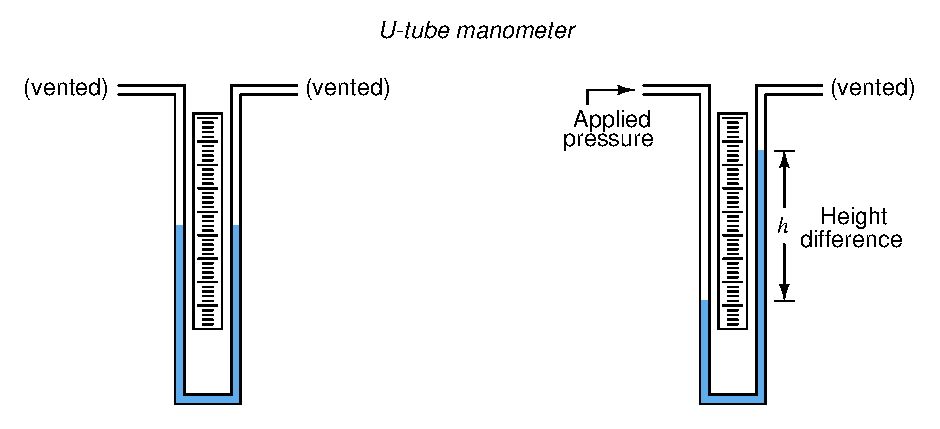
\includegraphics{pressure19.eps}$$
\begin{frame}
	\frametitle{Manometer}

	$$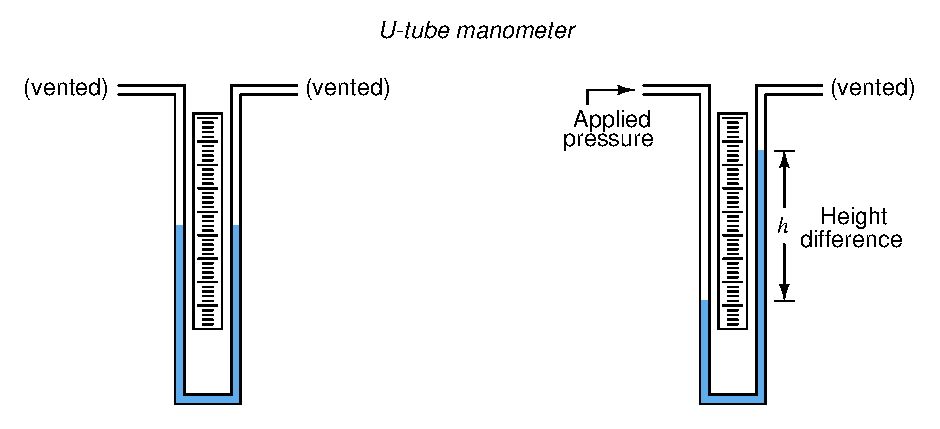
\includegraphics[height=6cm]{pressure19.eps}$$
$$P = \rho g h$$
\end{frame}

%
%The basis for all manometers is the mathematical relationship between a liquid's density ($\rho$ in mass units or $\gamma$ in weight units) and vertical height.  The diameter of the manometer tubes is irrelevant:
%
%$$P = \rho g h$$
%
%$$P = \gamma h$$
%
%Pressure is read on the scale as the difference in height ($h$) between the two liquid columns.  One nice feature of a manometer is it really cannot become ``uncalibrated'' so long as the fluid is pure and the assembly is maintained in an upright position.  If the fluid used is water, the manometer may be filled and emptied at will, and even rolled up for storage if the tubes are made of flexible plastic.
%
%\filbreak
%
%We may create even more sensitive manometers by purposely inclining one or more of the tubes, so that the liquid must travel a farther distance along the tube length to achieve the same vertical shift in height.  This has the effect of ``amplifying'' the liquid's motion to make it easier to resolve small pressures: \index{Inclined manometer} \index{Manometer, inclined}
%
%$$\includegraphics{pressure20.eps}$$
%
%This way, a greater motion of liquid ($x$) is required to generate the same hydrostatic pressure (vertical liquid displacement, $h$) than in an upright manometer, making the inclined manometer more sensitive.  As the similar triangle in the illustration shows, $x$ and $h$ are related trigonometrically by the sine function:
%
%$$\sin \theta = {h \over x}$$
%
%The difference in fluid column positions measured diagonally along the scale ($x$) must always be greater than the vertical height difference between the two columns ($h$) by a factor of $1 \over {\sin \theta}$, which will always be greater than one for angles less than 90$^{o}$.  The smaller the angle $\theta$, the greater the ratio between $x$ and $h$, leading to more sensitivity.
%
%\vskip 10pt
%
%\filbreak
%
%If even more sensitivity is desired, we may construct something called a \textit{micromanometer}, consisting of a gas bubble trapped in a clear horizontal tube between two large vertical manometer chambers: \index{Micromanometer}
%
%$$\includegraphics{pressure21.eps}$$
%
%Pressure applied to the top of either vertical chamber will cause the vertical liquid columns to shift just the same as any U-tube manometer.  However, the bubble trapped in the clear horizontal tube will move much farther than the vertical displacement of either liquid column, owing to the huge difference in cross-sectional area between the vertical chambers and the horizontal tube.  This amplification of motion is analogous to the amplification of motion in a hydraulic piston system (where the smaller piston moves farther than the larger piston), and makes the micromanometer exceptionally sensitive to small pressures.
%
%The movement of the gas bubble within the clear horizontal viewing tube ($x$) relates to applied pressure by the following formula:
%
%$$x = {{\gamma h} A_{large} \over {2 A_{small}}}$$
%
%\vskip 10pt
%
%Using water as the working liquid in a standard U-tube manometer, 1 PSI of applied gas pressure results in approximately 27.7 inches of vertical liquid column displacement (i.e. 27.7 inches of height \textit{difference} between the two water columns).  This relatively large range of motion limits the usefulness of water manometers to modest pressures only.  If we wished to use a water manometer to measure the pressure of compressed air in an industrial pneumatic supply system at approximately 100 PSI, the manometer would have to be in excess of 230 feet tall!  Clearly, a water manometer would not be the proper instrument to use for such an application.
%
%However, water is not the only viable liquid for use in manometers.  We could take the exact same clear U-tube and fill it partially full of liquid \textit{mercury} instead, which is substantially denser than water.  In a mercury manometer, 1 PSI of applied gas pressure results in very slightly more than 2 inches of liquid column displacement.  A mercury manometer applied to the task of measuring air pressure in an industrial pneumatic system would only have to be 17 feet tall -- still quite large and cumbersome\footnote{A colleague of mine told me once of working in an industrial facility with a very old steam boiler, where boiler steam pressure was actually indicated by tall mercury manometers reaching from floor to ceiling.  Operations personnel had to climb a ladder to accurately read pressure indicated by these manometers!} for a measuring instrument, but not impossible to construct or to use.
%
%\filbreak
%
%A common form of manometer seen in industrial instrument calibration shops is the \textit{well} type, consisting of a single vertical tube and a relatively large reservoir (called the ``well'') acting as the second column:
%
%$$\includegraphics{pressure22.eps}$$
%
%Due to the well's much larger cross-sectional area, liquid motion inside of it is negligible compared to the motion of liquid inside the clear viewing tube.  For all practical purposes\footnote{To give some perspective on just how little the liquid level changes in the well, consider a well-type manometer with a 1/4 inch (inside) diameter viewing tube and a 4-inch diameter circular well.  The ratio of diameters for these two liquid columns is 16:1, which means their ratio of areas is 256:1.  Thus, for every inch of liquid motion in the viewing tube, the liquid inside the well moves \textit{only $1 \over 256$ of an inch}.  Unless the viewing tube is quite tall, the amount of error incurred by interpreting the tube's liquid height directly as pressure will be minimal -- quite likely less than what the human eye is able to discern on a ruler scale anyway.  If the utmost accuracy is desired in a well manometer, however, we may compensate for the trifling motion of liquid in the well by building a custom ruler for the vertical tube -- one with a $255 \over 256$ reduced scale (so that $255 \over 256$ of an inch of liquid motion in the tube reads as exactly 1 inch of liquid column) in the case of the 1/4 inch tube and 4 inch well dimensions.}, the liquid level inside the ``well'' is constant, and so the liquid inside the tube moves the full distance equivalent to the applied pressure.  Thus, the well manometer provides an easier means of reading pressure: no longer does one have to measure the difference of height between \textit{two} liquid columns, only the height of a single column.
%
%
%
%
%
%
%
%\filbreak
%\subsection{Systems of pressure measurement}
%
%Pressure measurement is often a relative thing.  When we say there is 35 PSI of air pressure in an inflated car tire, what we mean is that the pressure inside the tire is 35 pounds per square inch \textit{greater than} the surrounding, ambient air pressure.  It is a fact that we live and breathe in a pressurized environment.  Just as a vertical column of liquid generates a hydrostatic pressure, so does a vertical column of gas.  If the column of gas is very tall, the pressure generated by it will be substantial.  Such is the case with Earth's atmosphere, the pressure at sea level caused by the weight of the atmosphere being approximately 14.7 PSI.
%
%You and I do not perceive this constant air pressure around us because the pressure inside our bodies is equal to the pressure outside our bodies.  Thus our eardrums, which serve as differential pressure-sensing diaphragms, detect no \textit{difference} of pressure between the inside and outside of our bodies.  The only time the Earth's air pressure becomes perceptible to us is if we rapidly ascend or descend, where the pressure inside our bodies does not have time to equalize with the pressure outside, and we feel the force of that differential pressure on our eardrums. \index{Differential pressure} \index{Pressure, differential}
%
%If we wish to speak of a fluid pressure in terms of how it compares to a perfect vacuum (absolute zero pressure), we specify it in terms of \textit{absolute} units.  For example, when I said earlier that the atmospheric pressure at sea level was 14.7 PSI, what I really meant is it is 14.7 PSIA (pounds per square inch \textit{absolute}), meaning 14.7 pounds per square inch \textit{greater than a perfect vacuum}.  When I said earlier that the air pressure inside an inflated car tire was 35 PSI, what I really meant is it was 35 PSIG (pounds per square inch \textit{gauge}), meaning 35 pounds per square inch \textit{greater than ambient air pressure}.  The qualifier ``gauge'' implies the pressure indicated by a pressure-measuring gauge, which in most cases works by comparing the sample fluid's pressure to that of the surrounding atmosphere.  When units of pressure measurement are specified without a ``G'' or ``A'' suffix, ``gauge'' pressure is usually\footnote{With few exceptions!} assumed.  \index{Absolute pressure}  \index{Pressure, absolute}  \index{Gauge pressure}  \index{Pressure, gauge}
%
%\filbreak
%
%Gauge and absolute pressure values for some common fluid pressures are shown in this table:
%
%% No blank lines allowed between lines of an \halign structure!
%% I use comments (%) instead, so that TeX doesn't choke.
%
%$$\vbox{\offinterlineskip
%\halign{\strut
%\vrule \quad\hfil # \ \hfil & 
%\vrule \quad\hfil # \ \hfil & 
%\vrule \quad\hfil # \ \hfil \vrule \cr
%\noalign{\hrule}
%%
%% First row
%\textbf{Gauge pressure} & \textbf{Fluid example} & \textbf{Absolute pressure} \cr
%%
%\noalign{\hrule}
%%
%% Another row
%90 PSIG & Bicycle tire air pressure & 104.7 PSIA \cr
%%
%\noalign{\hrule}
%%
%% Another row
%35 PSIG & Automobile tire air pressure & 49.7 PSIA \cr
%%
%\noalign{\hrule}
%%
%% Another row
%0 PSIG & Atmospheric pressure & 14.7 PSIA \cr
% & at sea level & \cr
%%
%\noalign{\hrule}
%%
%% Another row
%$-9.8$ PSIG & Engine manifold vacuum & 4.9 PSIA \cr
%(9.8 PSI vacuum) & under idle conditions & \cr
%%
%\noalign{\hrule}
%%
%% Another row
%$-14.7$ PSIG & Perfect vacuum & 0 PSIA \cr
%(14.7 PSI vacuum) & (no fluid molecules present) & \cr
%%
%\noalign{\hrule}
%%
%} % End of \halign 
%}$$ % End of \vbox
%
%Note that the only difference between each of the corresponding \textit{gauge} and \textit{absolute} pressures is an offset of 14.7 PSI, with absolute pressure being the larger (more positive) value.
%
%This offset of 14.7 PSI between \textit{absolute} and \textit{gauge} pressures can be confusing if we must convert between different pressure units.  Suppose we wished to express the tire pressure of 35 PSIG in units of inches of water column ("W.C.).  If we stay in the gauge-pressure scale, all we have to do is multiply by 27.68:
%
%$${{35 \> \hbox{\sout{PSI}}} \over 1} \times {{27.68 \> \hbox{"W.C.}} \over {1 \> \hbox{\sout{PSI}}}} = 968.8 \> \hbox{"W.C.}$$
%
%Note how the fractions have been arranged to facilitate cancellation of units.  The ``PSI'' unit in the numerator of the first fraction cancels with the ``PSI'' unit in the denominator of the second fraction, leaving inches of water column ("W.C.) as the only unit standing.  Multiplying the first fraction (35 PSI over 1) by the second fraction (27.68 "W.C. over 1 PSI) is ``legal'' to do since the second fraction has a \textit{physical} value of unity (1): being that 27.68 inches of water column is the same physical pressure as 1 PSI, the second fraction is really the number ``1'' in disguise.  As we know, multiplying any quantity by unity does not change its value, so the result of 968.8 "W.C. we get has the exact same physical meaning as the original figure of 35 PSI.  This technique of unit conversion is sometimes known as \textit{unity fractions}, and it is discussed in more general terms in another section of this book (refer to section \ref{Unit conversions} beginning on page \pageref{Unit conversions}).
%
%\vskip 10pt
%
%If, however, we wished to express the car's tire pressure in terms of inches of water column \textit{absolute} (in reference to a perfect vacuum), we would have to include the 14.7 PSI offset in our calculation, and do the conversion in two steps:
%
%$$35 \> \hbox{PSIG} + 14.7 \> \hbox{PSI} = 49.7 \> \hbox{PSIA}$$
%
%$${{49.7 \> \hbox{\sout{PSIA}}} \over 1} \times {{27.68 \> \hbox{"W.C.A}} \over {1 \> \hbox{\sout{PSIA}}}} = 1375.7 \> \hbox{"W.C.A}$$
%
%The ratio between inches of water column and pounds per square inch is still the same (27.68:1) in the absolute scale as it is in the gauge scale.  The only difference is that we included the 14.7 PSI offset in the very beginning to express the tire's pressure on the absolute scale rather than on the gauge scale.  From then on, all conversions were performed in absolute units.
%
%This two-step conversion process is not unlike converting between different units of temperature (degrees Celsius versus degrees Fahrenheit), and for the exact same reason.  To convert from $^{o}$F to $^{o}$C, we must first \textit{subtract} an offset of 32 degrees, then \textit{multiply} by $5 \over 9$.  The reason an offset is involved in this temperature conversion is because the two temperature scales do not share the same ``zero'' point: 0 $^{o}$C is \textit{not} the same temperature as 0 $^{o}$F.  Likewise, 0 PSIG is \textit{not} the same pressure as 0 PSIA, and so an offset is always necessary to convert between gauge and absolute pressure units.
%
%\vskip 10pt
%
%\filbreak
%
%As seen with the unit of pounds per square inch (PSI), the distinction between gauge and absolute pressure is typically shown by a lettered suffix ``G'' or ``A'' following the unit, respectively.  Following this convention, we may encounter other units of pressure measurement qualified as either gauge or absolute by these letters: kPaA (kilopascals absolute), inches HgG (inches of mercury gauge), inches W.C.A (inches of water column absolute), etc.  
%
%There are some pressure units that are \textit{always} in absolute terms, and as such require no letter ``A'' to specify.  One is the unit of \textit{atmospheres}, 1 atmosphere being 14.7 PSIA.  There is no such thing as ``atmospheres gauge'' pressure.  For example, if we were given a pressure as being 4.5 atmospheres and we wanted to convert that into pounds per square inch gauge (PSIG), the conversion would be a two-step process: \index{Atmospheres}
%
%$${{4.5 \> \hbox{\sout{atm}}} \over 1} \times {{14.7 \> \hbox{PSIA}} \over {1 \> \hbox{\sout{atm}}}} = 66.15 \> \hbox{PSIA}$$
%
%$$66.15 \> \hbox{PSIA} - 14.7 \> \hbox{PSI} = 51.45 \> \hbox{PSIG}$$
%
%Another unit of pressure measurement that is always absolute is the \textit{torr}, equal to 1 millimeter of mercury column absolute (mmHgA).  0 torr is absolute zero, equal to 0 atmospheres, 0 PSIA, or $-14.7$ PSIG.  Atmospheric pressure at sea level is 760 torr, equal to 1 atmosphere, 14.7 PSIA, or 0 PSIG. \index{Torr}
%
%If we wished to convert the car tire's pressure of 35 PSIG into torr, we would once again have to offset the initial value to get everything into absolute terms.
%
%$$35 \> \hbox{PSIG} + 14.7 \> \hbox{PSI} = 49.7 \> \hbox{PSIA}$$
%
%$${{49.7 \> \hbox{\sout{PSIA}}} \over 1} \times {{760 \> \hbox{torr}} \over {14.7 \> \hbox{\sout{PSIA}}}} = 2569.5 \> \hbox{torr}$$
%
%\vskip 10pt
%
%One last unit of pressure measurement deserves special comment, for it may be used to express either gauge or absolute pressure, yet it is \textit{not} customary to append a ``G'' or an ``A'' to the unit.  This unit is the \textit{bar}, exactly equal to 100 kPa, and approximately equal\footnote{The origin of this unit for pressure is the atmospheric pressure at sea level: 1 atmosphere, or 14.7 PSIA.  The word ``bar'' is short for \textit{barometric}, in reference to Earth's ambient atmospheric pressure.} to 14.5 PSI.  Some technical references append a lower-case letter ``g'' or ``a'' to the word ``bar'' to show either gauge pressure (\textit{barg}) or absolute pressure (\textit{bara}), but this notation seems no longer favored.  Modern usage typically omits the ``g'' or ``a'' suffix in favor of context: the word ``gauge'' or ``absolute'' may be included in the expression to clarify the meaning of ``bar.''  Sadly, many references fail to explicitly declare either ``gauge'' or ``absolute'' when using units of \textit{bar}, leaving the reader to interpret the intended context.  Despite this ambiguity, the \textit{bar} is frequently used in European literature as a unit of pressure measurement.  \index{Bar}  \index{Barg}  \index{Bara}
%
%
%
%
%
%
%
%\filbreak
%\subsection{Negative pressure}
%
%\index{Negative pressure}  \index{Pressure, negative}
%
%If a chamber is completely evacuated of any and all fluid molecules such that it contains nothing but empty space, we say that it contains a perfect \textit{vacuum}.  With no fluid molecules inside the chamber whatsoever, there will be no pressure exerted on the chamber walls by any fluid.  This is the defining condition of zero absolute pressure (e.g. 0 PSIA, 0 torr, 0 atmospheres, etc.).  Referencing atmospheric air pressure\footnote{At sea level, where the absolute pressure is 14.7 PSIA.  Atmospheric pressure will be different at different elevations above (or below) sea level.} outside of this vessel, we could say that the ``gauge'' pressure of a perfect vacuum is $-14.7$ PSIG.
%
%A commonly-taught principle is that a perfect vacuum is the lowest pressure possible in any physical system.  However, this is not strictly true.  It is, in fact, possible to generate pressures \textit{below} 0 PSIA -- pressures that are actually \textit{less} than that of a perfect vacuum.  The key to understanding this is to consider non-gaseous systems, where the pressure in question exists within a solid or a liquid substance.
%
%\vskip 10pt
%
%Let us begin our exploration of this concept by considering the case of weight applied to a solid metal bar: \index{Pressure, within solids}
%
%$$\includegraphics{fluids_36.eps}$$
%
%Recall that pressure is defined as force exerted over area.  This metal bar certainly has a cross-sectional area, and if a compressive force is applied to the bar then the molecules of metal inside the bar will experience a pressure attempting to force them closer together.  Supposing the bar in question measured 1.25 inches wide and thick, its cross-sectional area would be (1.25 in)$^{2}$, or 1.5625 in$^{2}$.  Applying a force of 80 pounds along the bar's length would set up an internal pressure within the bar of 51.2 pounds per square inch, or 51.2 PSI:
%
%$$\includegraphics{fluids_37.eps}$$
%
%\filbreak
%
%Now suppose we reverse the direction of the applied force to the bar, applying \textit{tension} to the bar rather than \textit{compression}.  If the force is still 80 pounds and the cross-sectional area is still 1.5625 square inches, then the internal pressure inside the bar must be $-51.2$ PSI:
%
%$$\includegraphics{fluids_38.eps}$$
%
%The negative pressure value describes the tensile force experienced by the molecules of metal inside the bar: a degree of force per unit area attempting to pull those molecules apart from each other rather than push them closer together as was the case with a compressive force.
%
%If you believe that the lowest possible pressure is a perfect vacuum (0 PSIA, or $-14.7$ PSIG), then this figure of $-51.2$ PSI seems impossible.  However, it is indeed possible because we are dealing with a solid rather than with a gas.  Gas molecules exert pressure on a surface by striking that surface and exerting a force by the momentum of their impact.  Since gas molecules can only strike (i.e. \textit{push}) against a surface, and cannot \textit{pull} against a surface, one cannot generate a negative absolute pressure using a gas.  In solids, however, the molecules comprising the sample exhibit \textit{cohesion}, allowing us to set up a tension within that material impossible in a gaseous sample where there is no cohesion between the molecules.  Thus, negative pressures are possible within samples of solid material even though they are impossible within gases.
%
%\vskip 10pt
%
%Negative pressures are also possible within \textit{liquid} samples, provided there are no bubbles of gas or vapor anywhere within the sample.  Like solids, the molecules within a liquid also exhibit cohesion (i.e. they tend to ``stick'' together rather than drift apart from each other).  If a piston-and-cylinder arrangement is completely filled with liquid, and a tension applied to the movable piston, the molecules within that liquid will experience tension as well.  Thus, it is possible to generate negative pressures (below 0 PSIA) within liquids that are impossible with gases.
%
%Even vertical columns of liquid may generate negative pressure.  The famous British scientists Hooke and Boyle demonstrated a negative pressure of $-0.2$ MPa ($-29$ PSI) using a column of liquid mercury.  Trees naturally generate huge negative pressures in order to draw water to their full height, up from the ground.  Two scientists, H.H. Dixon and J. Joly, presented a scientific paper entitled \textit{On the Ascent of Sap} in 1895 proposing liquid tension as the mechanism by which trees could draw water up tremendous heights.
%
%If even the smallest bubble of gas exists within a liquid sample, however, negative pressures become impossible.  Since gases can only exert positive pressures, and Pascal's Principle tells us that pressure will be equally distributed throughout a fluid sample, the low-limit of 0 PSIA for gases establishes a low pressure limit for the entire liquid/gas sample.  In other words, the presence of any gas within an otherwise liquid sample prevents the entire sample from experiencing tension.
%
%\vskip 10pt

%One limitation to the generation of negative pressures within liquids is that disturbances and/or impurities within the liquid may cause that liquid to spontaneously boil (changing phase from liquid to vapor), at which point a sustained negative pressure becomes impossible.






%\chapter{Continuous pressure measurement}

%In many ways, pressure is the primary variable for a wide range of process measurements.  Many types of industrial measurements are actually inferred from pressure, such as:  \index{Inferred variable}
%
%\begin{itemize}
%\item Flow (measuring the pressure dropped across a restriction)
%\item Liquid level (measuring the pressure created by a vertical liquid column)
%\item Liquid density (measuring the pressure difference across a fixed-height liquid column)
%\item Weight (hydraulic load cell)
%\end{itemize}
%
%Even temperature may be inferred from pressure measurement, as in the case of a fluid-filled chamber where fluid pressure and fluid temperature are directly related.  As such, pressure is a very important quantity to measure, and measure accurately.  This section describes different technologies for the measurement of pressure.  \index{Inferred variable}
%
%
%
%
%
%
%\filbreak
%\section{Manometers}
%
%A very simple device used to measure pressure is the \textit{manometer}: a fluid-filled tube where an applied gas pressure causes the fluid height to shift proportionately.  This is why pressure is often measured in units of liquid height (e.g. inches of water, inches of mercury).  As you can see, a manometer is fundamentally an instrument of \textit{differential} pressure measurement, indicating the difference between two pressures by a shift in liquid column height: \index{Manometer}
%
%$$\includegraphics{005.eps}$$
\begin{frame}
	\frametitle{Manometer}

	$$\includegraphics[height=7cm]{005.eps}$$
\end{frame}

%
%Of course, it is entirely acceptable to simply vent one tube of a manometer and use it as a \textit{gauge} pressure instrument, comparing the applied pressure at one tube against atmospheric pressure in the other.
%
%\filbreak
%
%Liquid column height in a manometer should always be interpreted at the centerline of the liquid column, regardless of the shape of the liquid's meniscus (the curved air/liquid interface): \index{Meniscus}
%
%$$\includegraphics{006.eps}$$
\begin{frame}
	\frametitle{Avlesning av manometer}

	$$\includegraphics[height=7cm]{006.eps}$$
\end{frame}

%
%\filbreak
%
%Manometers come in a variety of forms, the most common being the \textit{U-tube}, \textit{well} (sometimes called a \textit{cistern}), \textit{raised well}, and \textit{inclined}: \index{Manometer, U-tube} \index{Manometer, well} \index{Manometer, raised well} \index{Manometer, inclined} \index{Inclined manometer} \index{U-tube manometer} \index{Well manometer}  \index{Raised well manometer}  \index{Cistern manometer} \index{Manometer, cistern}
%
%$$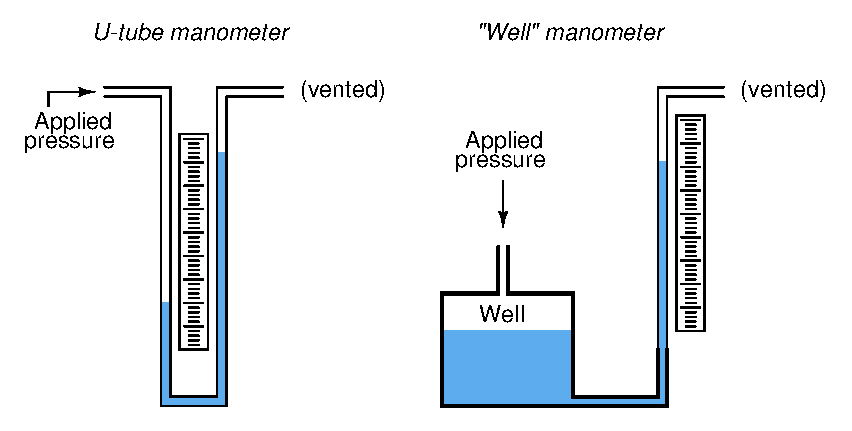
\includegraphics{007.eps}$$
%
%$$\includegraphics{008.eps}$$
%
%\filbreak
%
%U-tube manometers are very inexpensive, and are generally made from clear plastic (see the left-hand photo).  Cistern-style manometers are the norm for calibration bench work, and are typically constructed from metal cisterns and glass tubes (see the right-hand photo):
%
%$$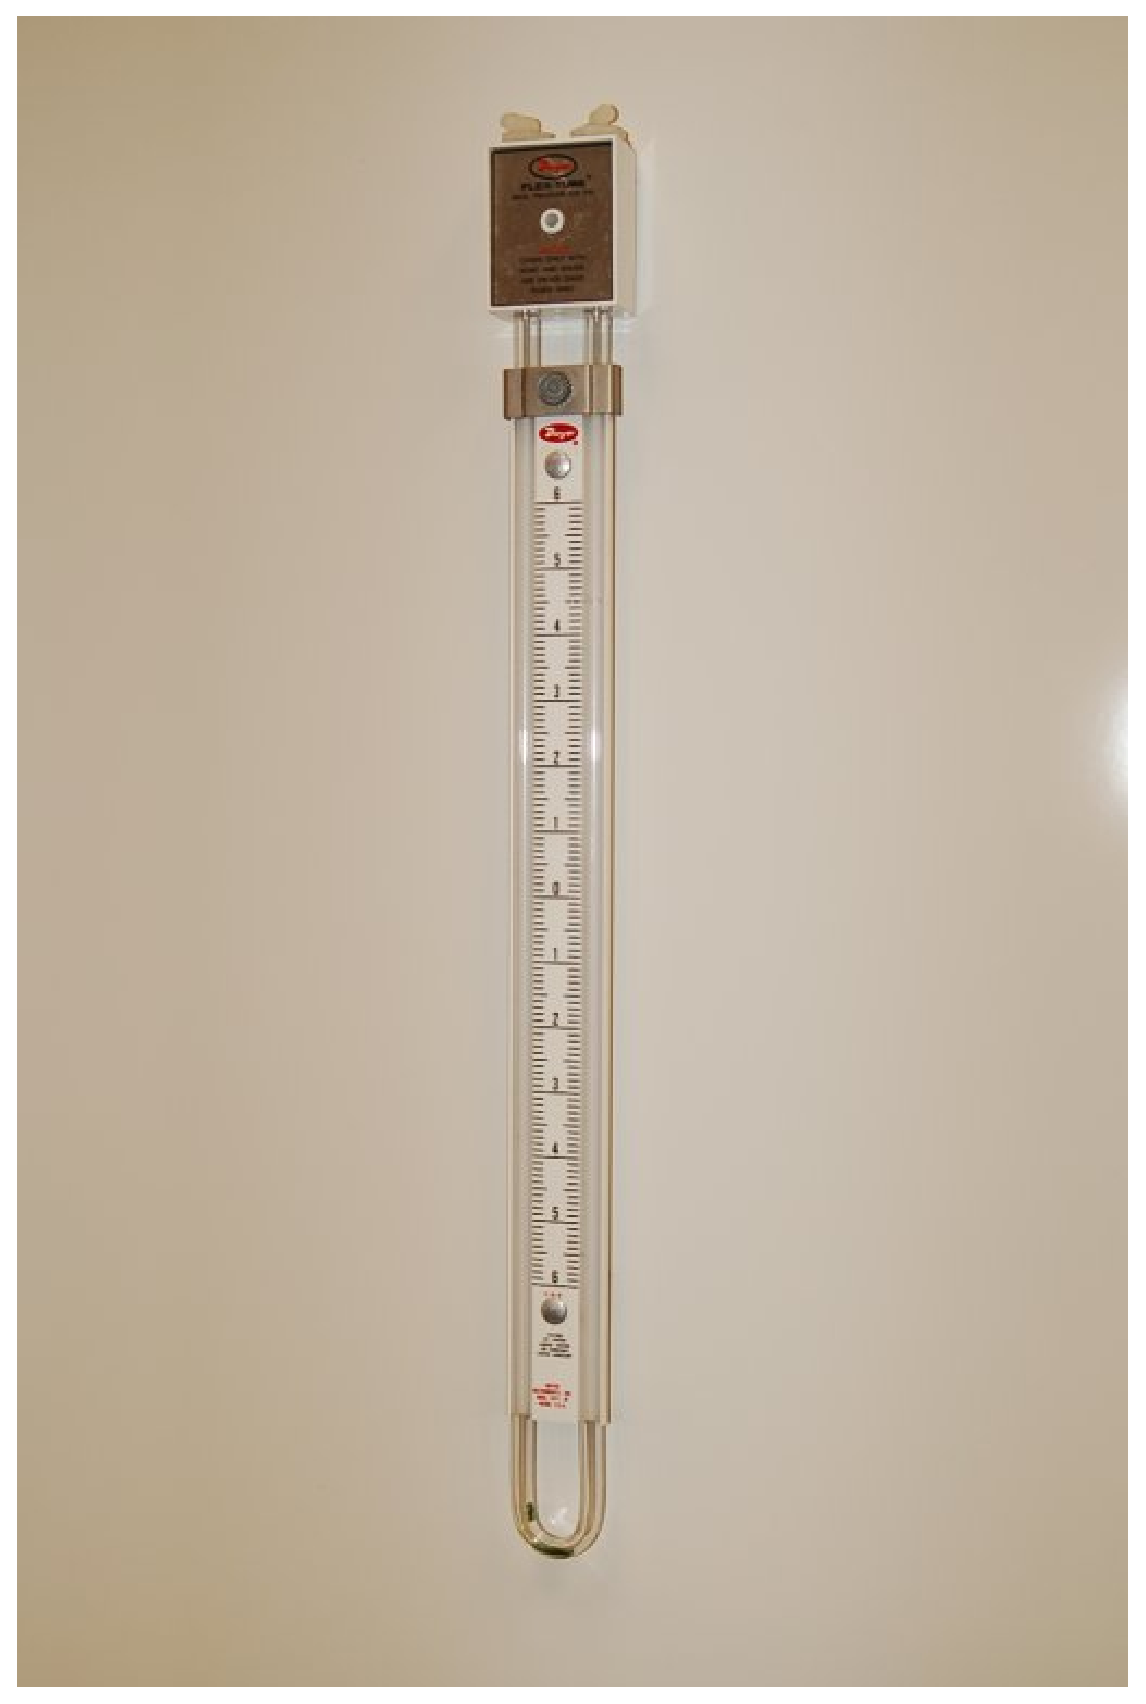
\includegraphics[width=2in]{u_tube_manometer.eps} \hskip 30pt 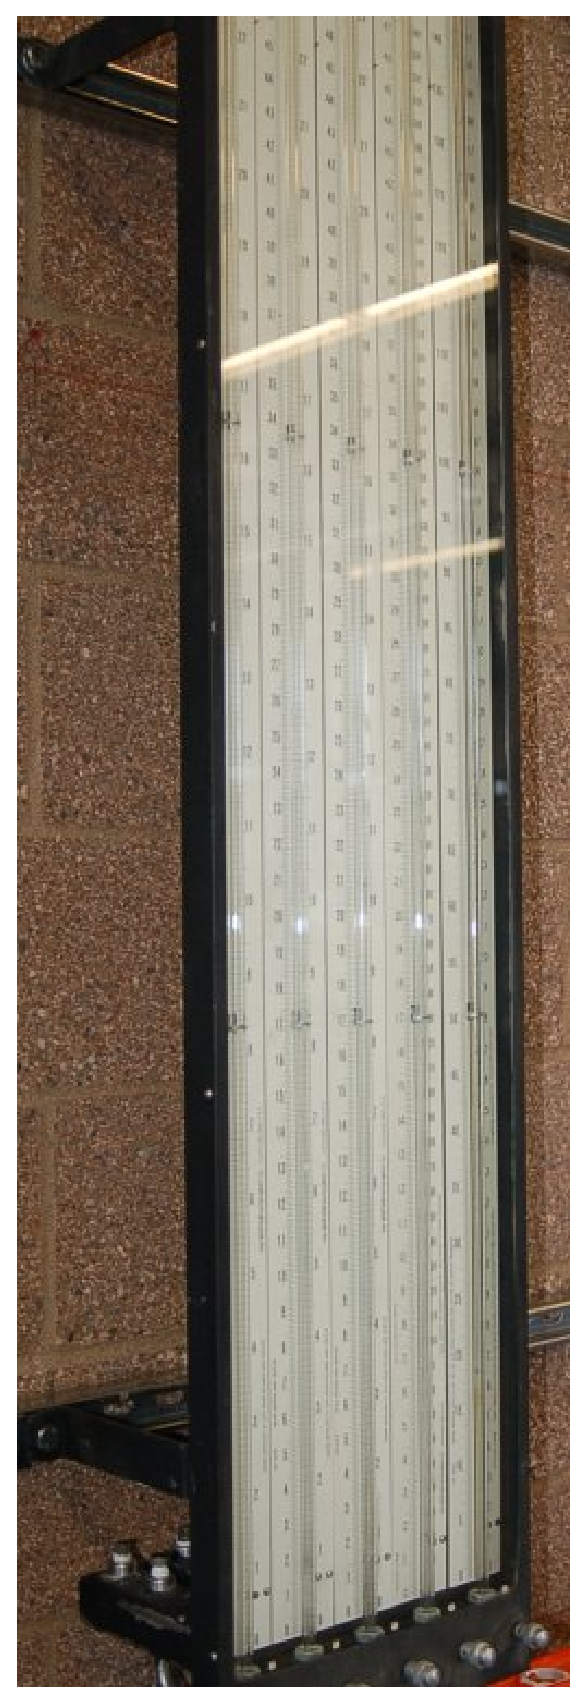
\includegraphics[width=2in]{cistern_manometers.eps}$$
%
%\filbreak
%
%Inclined manometers are used to measure very low pressures, owing to their exceptional sensitivity (note the fractional scale for inches of water column in the following photograph, extending from 0 to 1.5 inches on the scale, reading left to right):
%
%$$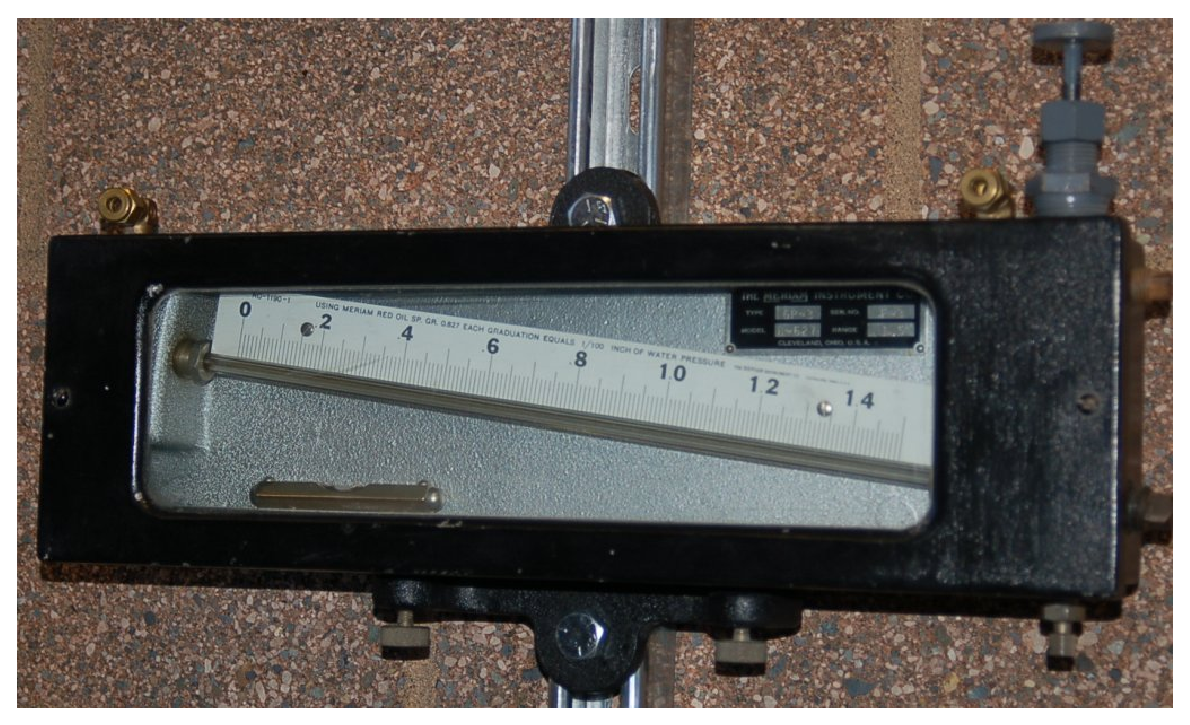
\includegraphics[width=5in]{inclined_manometer.eps}$$
%
%Note that venting one side of a manometer is standard practice when using it as a \textit{gauge pressure} indicator (responding to pressure in excess of atmospheric).  Both pressure ports will be used if the manometer is applied to the measurement of differential pressure, just as in the case of the U-tube manometer first shown in this section.  Absolute pressure may also be measured by a manometer, if one of the pressure ports connects to a sealed vacuum chamber.  This is how a \textit{mercury barometer} is constructed for the measurement of absolute ambient air pressure: by sealing off one side of a manometer and removing all the air in that side, such that the applied (atmospheric) pressure is always compared against a vacuum. \index{Barometer} \index{Mercury barometer} \index{Absolute pressure} \index{Differential pressure} \index{Gauge pressure}
%
%Manometers incorporating a ``well'' have the advantage of single-point reading: one need only compare the height of \textit{one} liquid column, not the difference in height between \textit{two} liquid columns.  The cross-sectional area of the liquid column in the well is so much greater than that within the transparent manometer tube that the change in height within the well is usually negligible.  In cases where the difference is significant, the spacing between divisions on the manometer scale may be skewed to compensate\footnote{If you are having difficulty understanding this concept, imagine a simple U-tube manometer where one of the tubes is opaque, and therefore one of the two liquid columns cannot be seen.  In order to be able to measure pressure just by looking at one liquid column height, we would have to make a custom scale where every inch of height registered as \textit{two} inches of water column pressure, because for each inch of height change in the liquid column we can see, the liquid column we can't see also changes by an inch.  A scale custom-made for a well-type manometer is just the same concept, only without such dramatic skewing of scales.}.
%
%Inclined manometers enjoy the advantage of increased sensitivity.  Since manometers fundamentally operate on the principle of pressure balanced by liquid height, and this liquid height is always measured parallel to the line of gravitational pull (perfectly vertical), inclining the manometer tube means that liquid must travel farther along the tube to generate the same change in (purely) vertical height than it would in a vertical manometer tube.  Thus, an inclined manometer tube causes an amplification in liquid motion for a given amount of pressure change, allowing measurements of greater resolution.
%
%
%
%
%
%\filbreak
%\section{Mechanical pressure elements}
%
%Mechanical pressure-sensing elements include the \textit{bellows}, the \textit{diaphragm}, and the \textit{bourdon tube}.  Each of these devices converts a fluid pressure into a force.  If unrestrained, the natural elastic properties of the element will produce a motion proportional to the applied pressure.  \index{Bellows} \index{Diaphragm} \index{Bourdon tube}
%
%$$\includegraphics{003.eps}$$
\begin{frame}
	\frametitle{Mekaniske trykksensorer}

	$$\includegraphics[width=1\textwidth]{003.eps}$$
\end{frame}

%
%Bellows resemble an accordion constructed from metal instead of fabric.  Increasing pressure inside a bellows unit causes it to elongate.  A photograph of a bellows is shown here:
%
%$$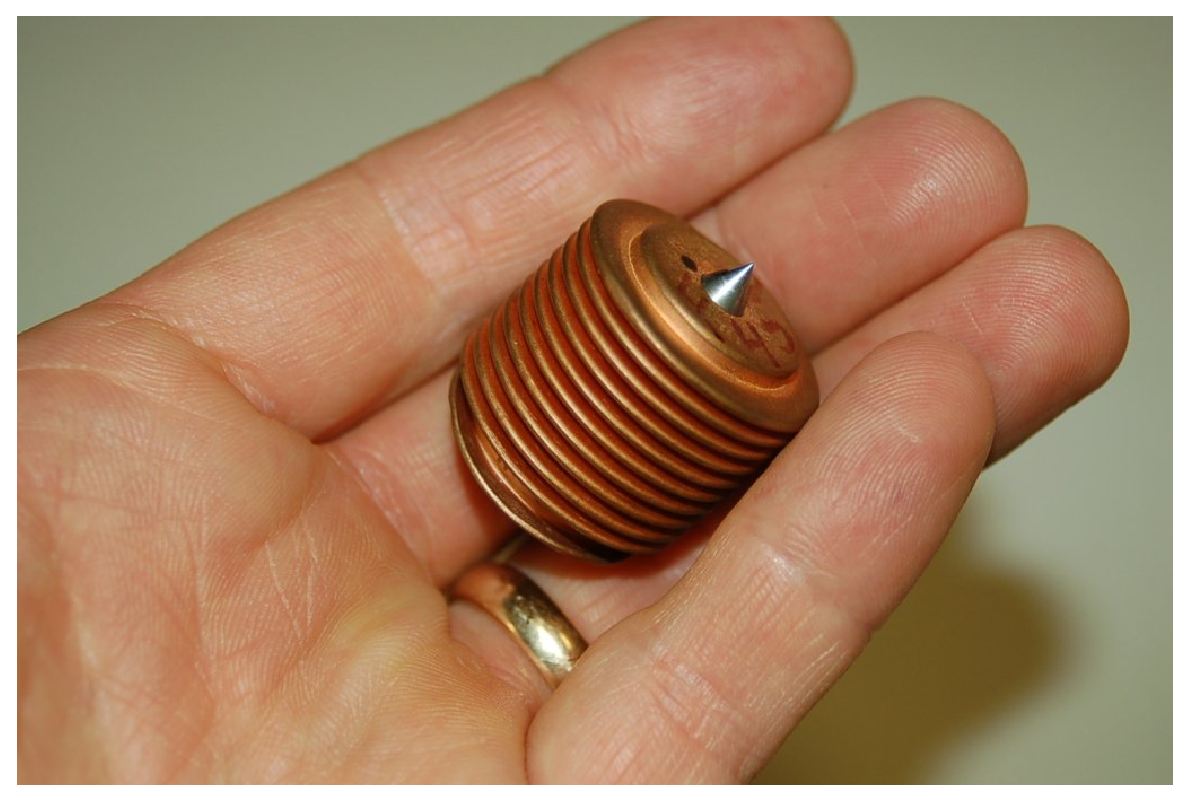
\includegraphics[width=4in]{pneumatics35.eps}$$
%
%A diaphragm is nothing more than a thin disk of material which bows outward under the influence of a fluid pressure.  Many diaphragms are constructed from metal, which gives them spring-like qualities.  Some diaphragms are intentionally constructed out of materials with little strength, such that there is negligible spring effect.  These are called \textit{slack diaphragms}, and they are used in conjunction with external mechanisms (e.g. springs) producing the necessary restraining force to prevent damage from applied pressure.  \index{Slack diaphragm} 
%
%\filbreak
%
%The following photograph shows the mechanism of a small pressure gauge using a brass diaphragm as the sensing element:
%
%$$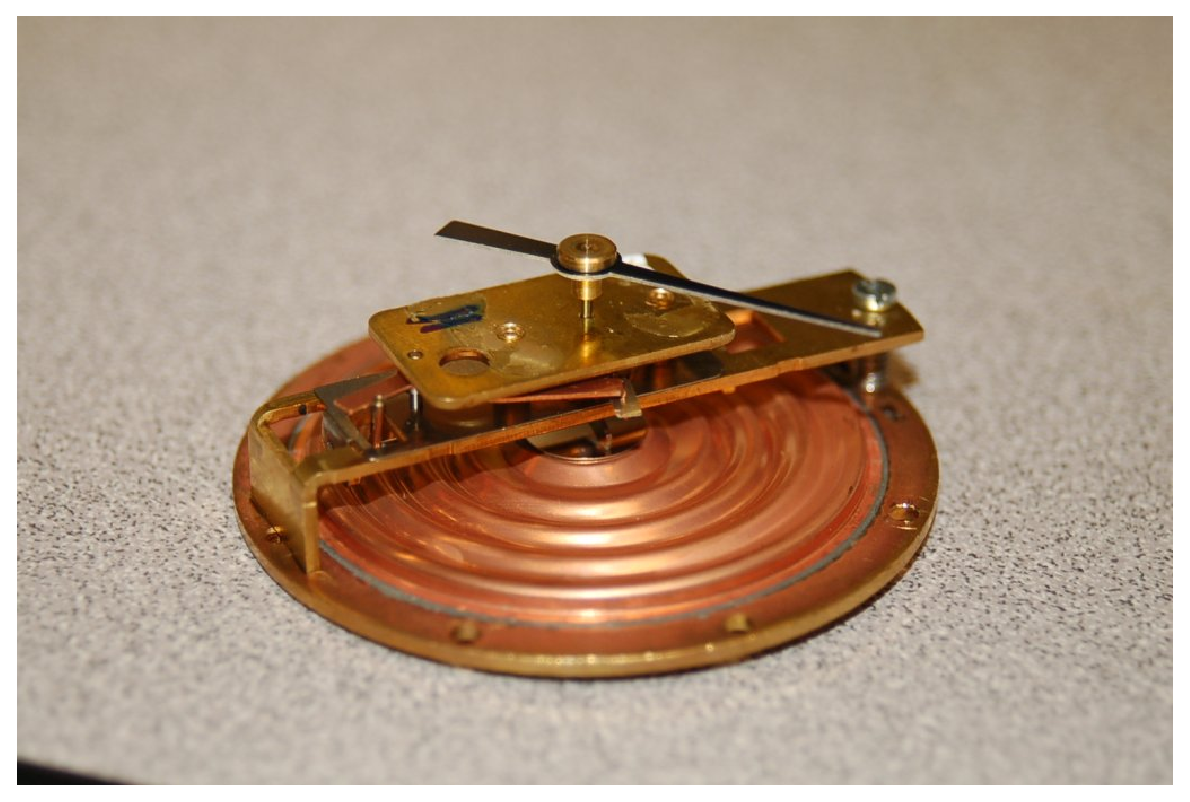
\includegraphics[width=5in]{gauge_diaphragm.eps}$$
\begin{frame}
	\frametitle{}

	$$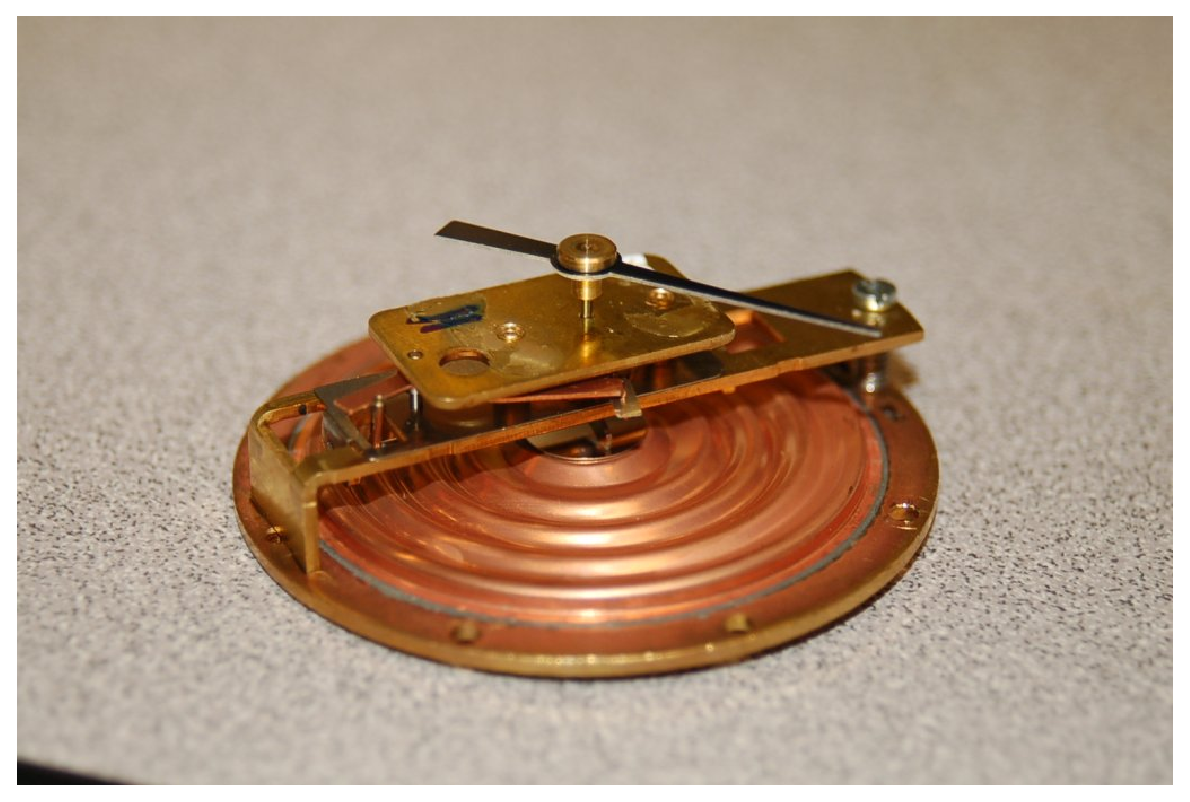
\includegraphics[height=7cm]{./gauge_diaphragm.eps}$$
\end{frame}

%
%As pressure is applied to the rear of the diaphragm, it distends upward (away from the table on which it rests as shown in the photograph), causing a small shaft to twist in response.  This twisting motion is transferred to a lever which pulls on a tiny link chain wrapped around the pointer shaft, causing it to rotate and move the pointer needle around the gauge scale.  Both the needle and scale on this gauge mechanism have been removed for easier viewing of diaphragm and mechanism.
%
%\vskip 10pt
%
%Bourdon tubes are made of spring-like metal alloys bent into a circular shape.  Under the influence of internal pressure, a bourdon tube ``tries'' to straighten out into its original shape before being bent at the time of manufacture.
%
%Most pressure gauges use a bourdon tube as their pressure-sensing element.  Most pressure transmitters use a diaphragm as their pressure-sensing element.  Bourdon tubes may be made in \textit{spiral} or \textit{helical} forms for greater motion (and therefore greater gauge resolution).  \index{Helical bourdon tube} \index{Spiral bourdon tube}
%
%\filbreak
%
%The Bourdon tube pressure element is a very robust and time-tested design.  An illustration taken from page 471 of volume 1 of \textit{Cassier's Magazine} published in the year 1891 shows a typical C-shaped bourdon tube pressure gauge mechanism complete with gears and pointing needle:  \index{Pressure gauge mechanism, typical}  \index{Bourdon tube}
%
%$$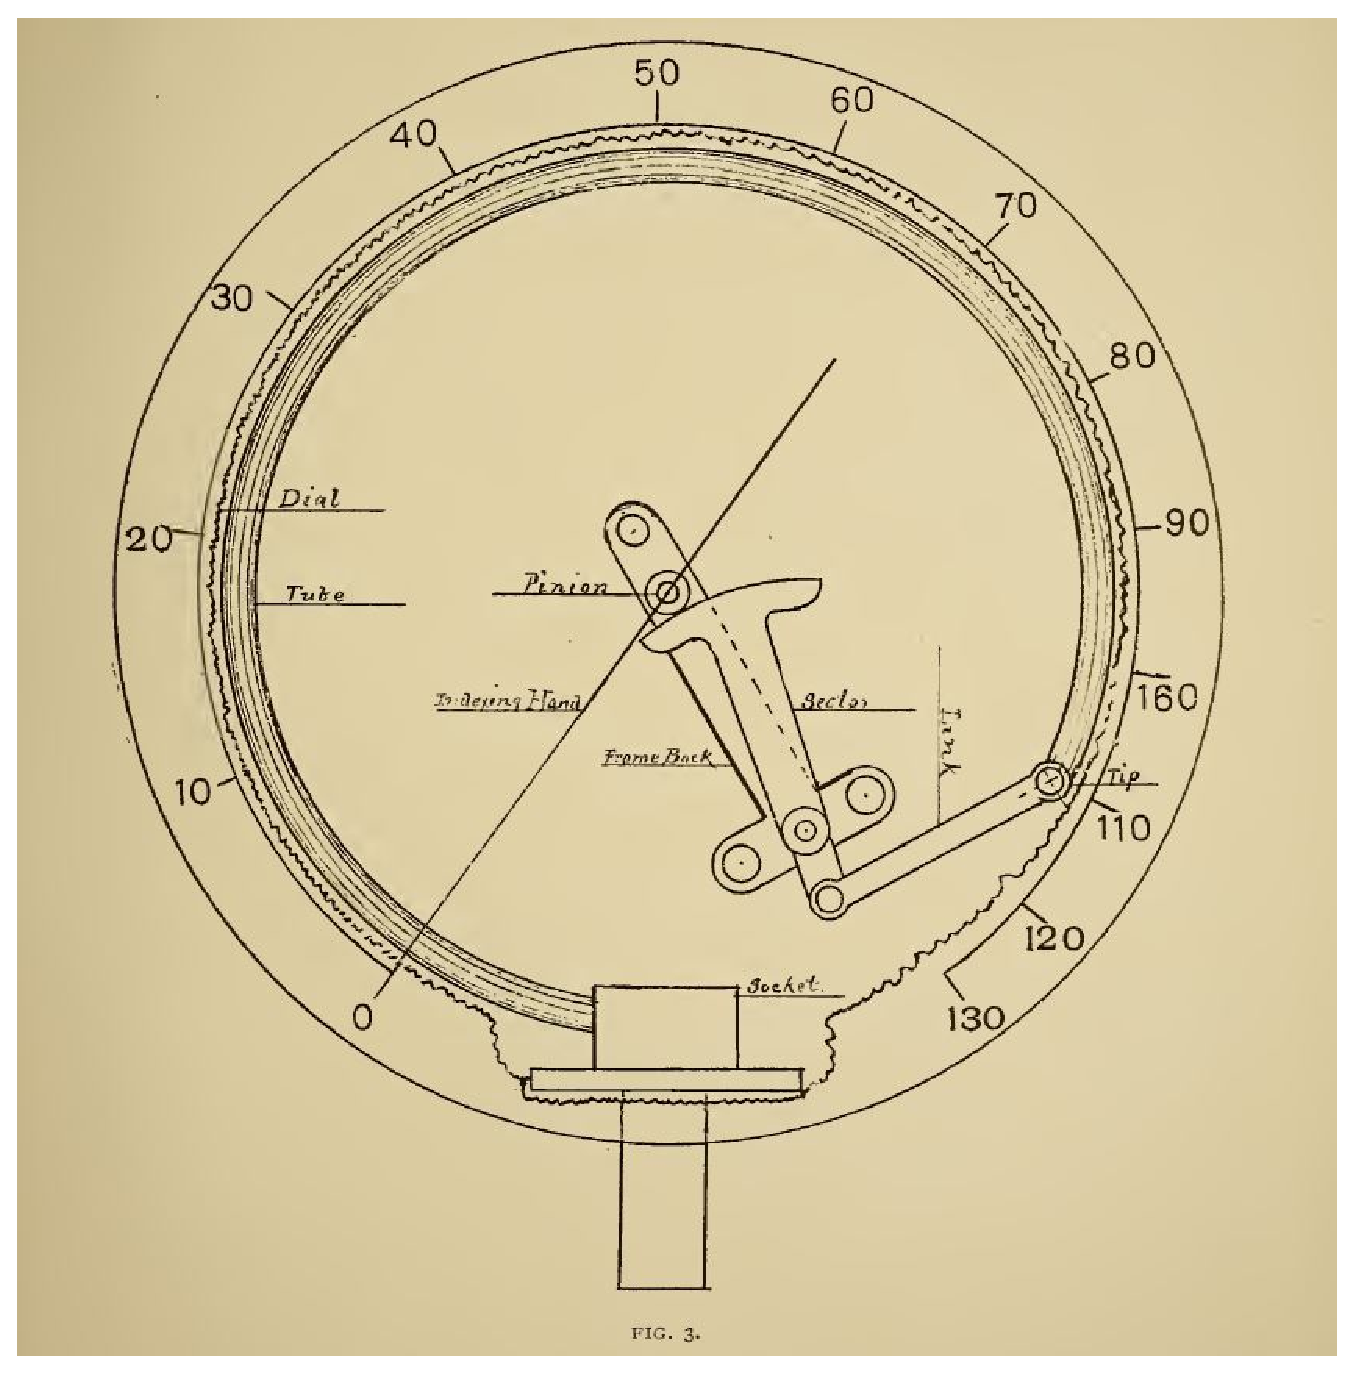
\includegraphics[height=6in]{020.eps}$$
\begin{frame}
	\frametitle{Bourdon rør}

	$$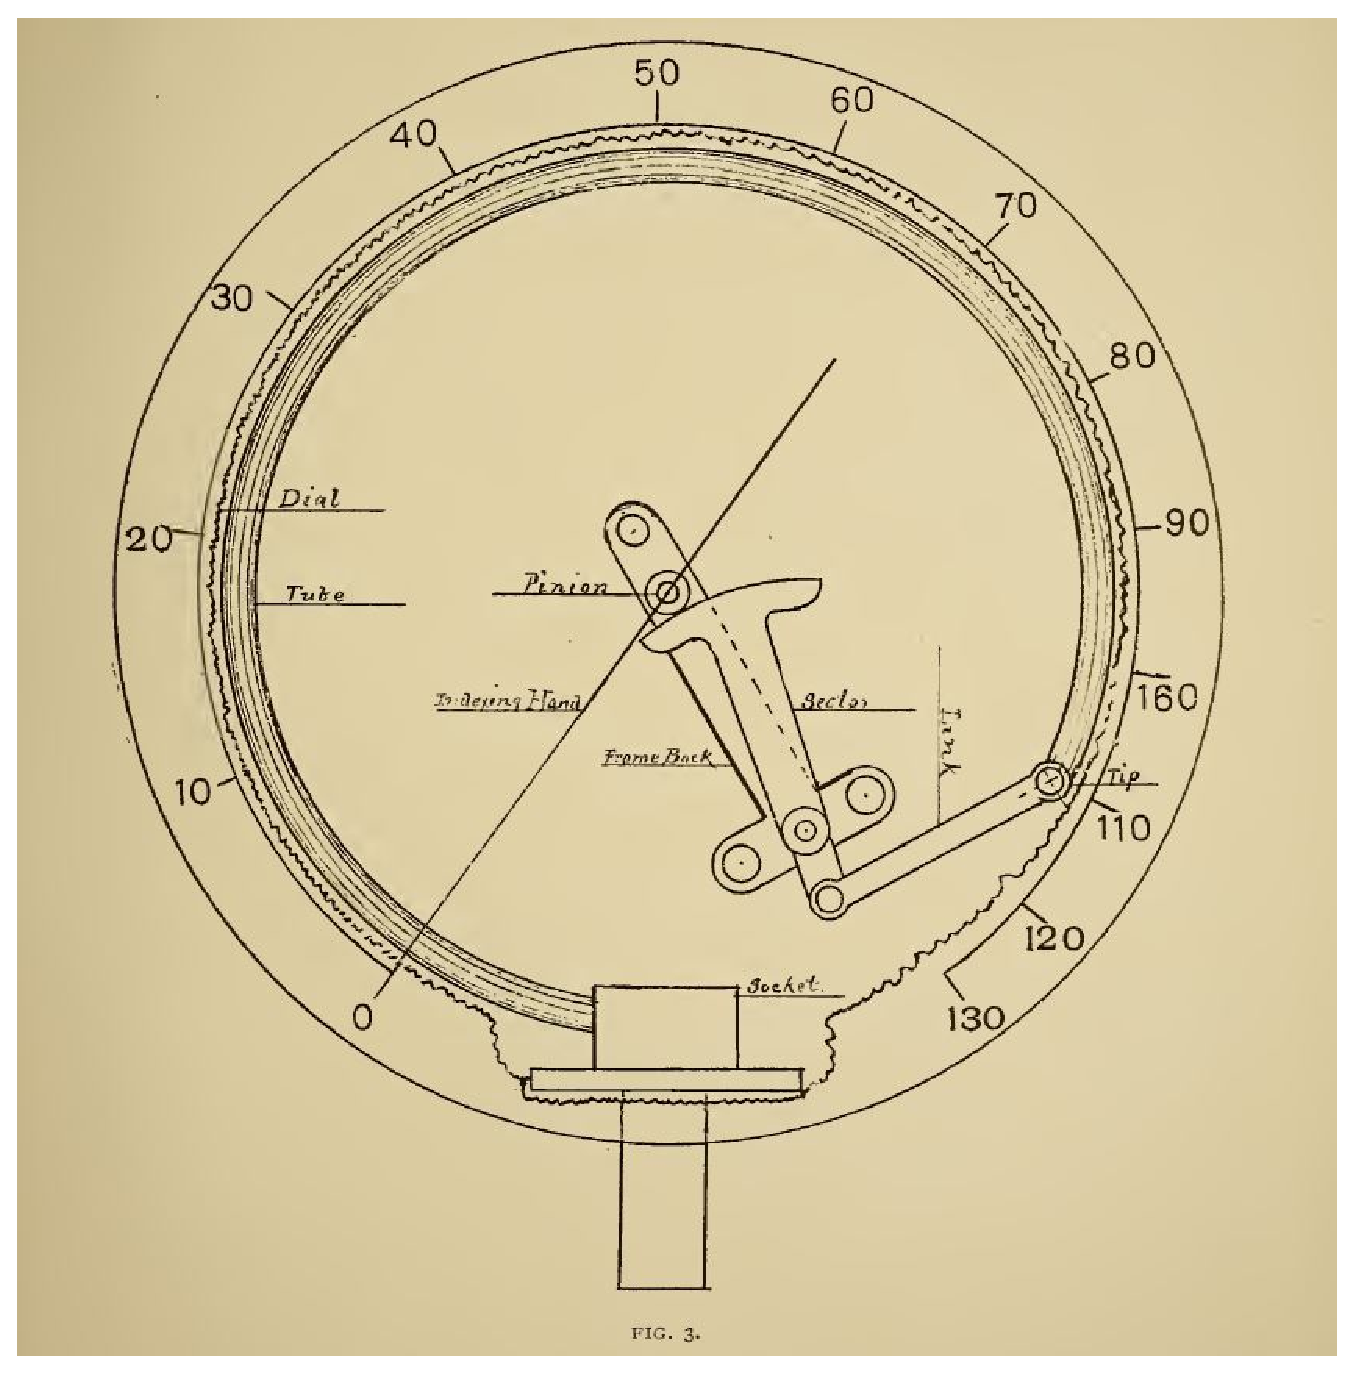
\includegraphics[height=7cm]{020.eps}$$
\end{frame}

%
%Looking closely at the labeled components of this mechanism, we see a circular ``pinion'' touching a curved ``sector''.  Both of these are \textit{gears} meshing with one another, but as is typical with mechanical drawings the individual teeth of the meshing gears are not shown.
%
%It is a useful mental exercise to imagine the components of this gauge moving under the influence of a rising fluid pressure.  The bourdon tube will straighten, resulting in its tip extending outward from center (up and right) as its socket remains stationary (anchored to the gauge body).  This pulls on the link, which in turn causes the sector gear to rotate counter-clockwise on its bearing axis (that axis anchored on the backing plate of the gauge).  This causes the pinion gear to rotate clockwise, driving the needle (the ``indexing hand'') clockwise as well, so that the needle's tip rises up the numerical scale printed on the gauge face.
%
%\filbreak
%
%A photograph of a C-tube pressure gauge mechanism (taken from the rear of the gauge, behind the pointer and scale) reveals its mechanical workings:
%
%$$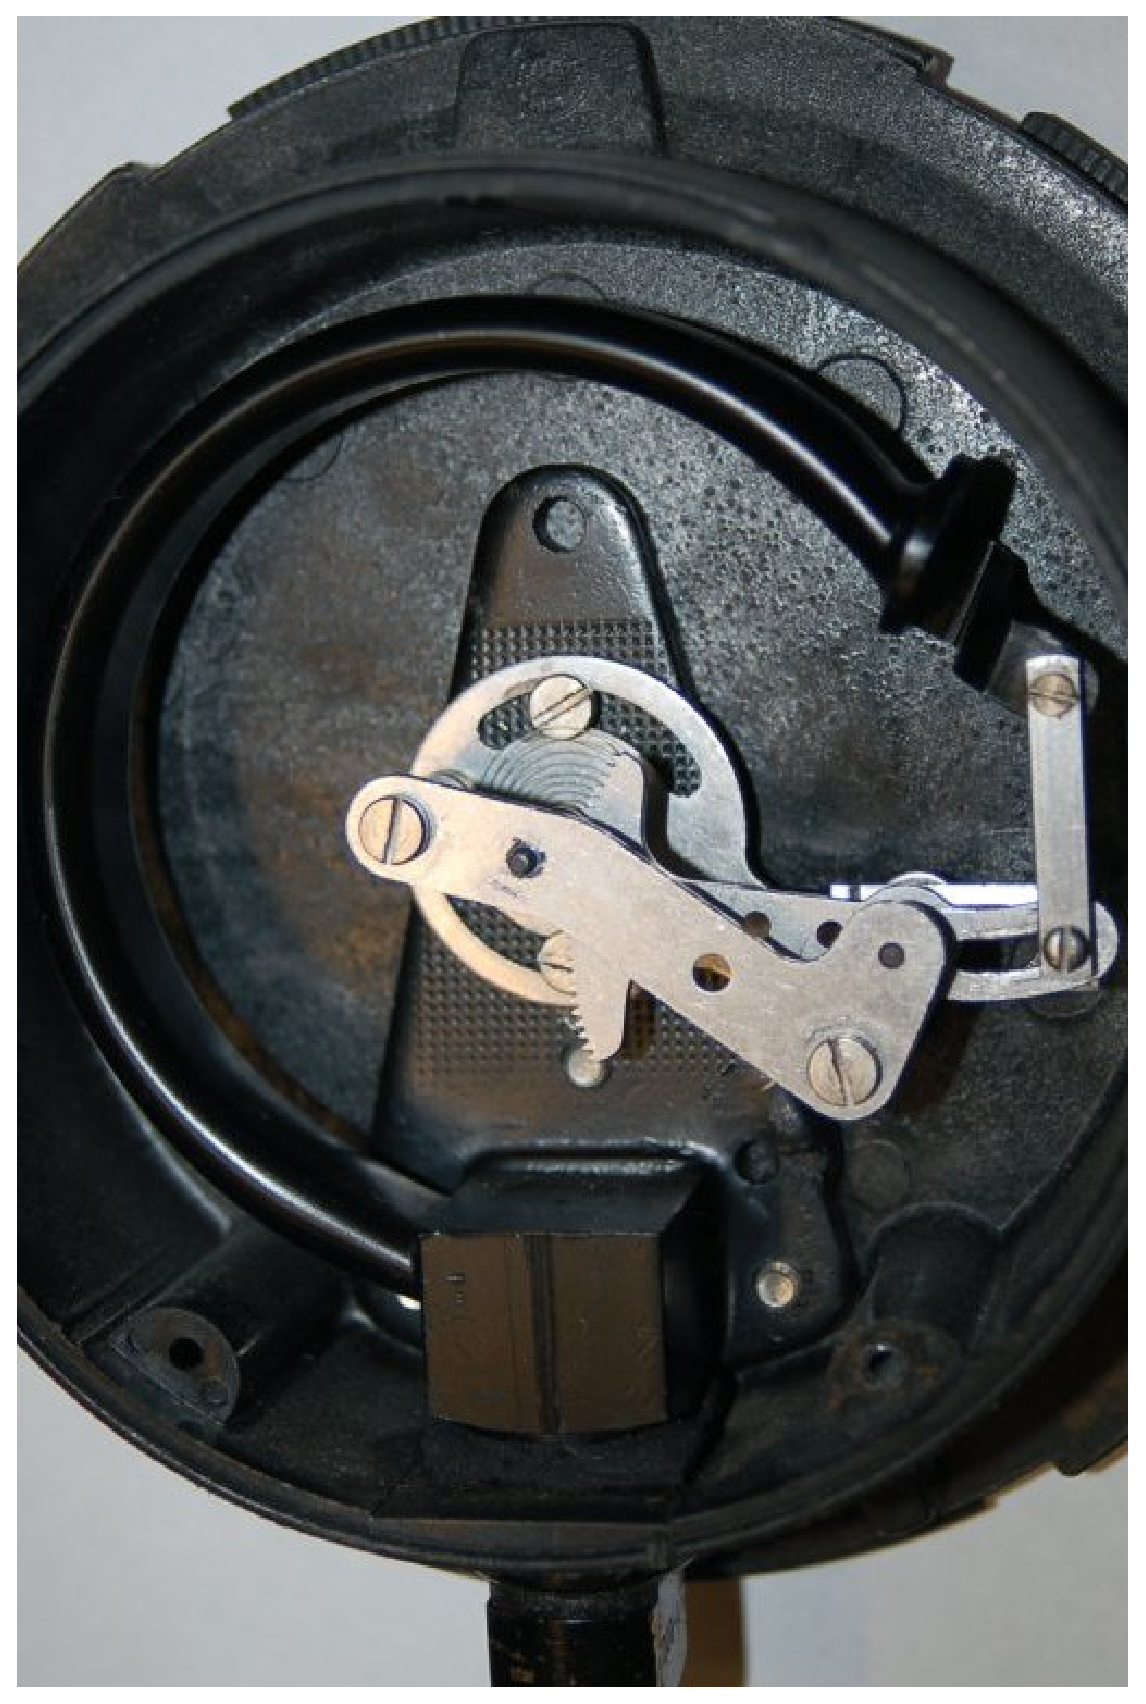
\includegraphics[width=3in]{bourdon_tube_closeup.eps}$$
\begin{frame}
	\frametitle{Bourdon rør}

	$$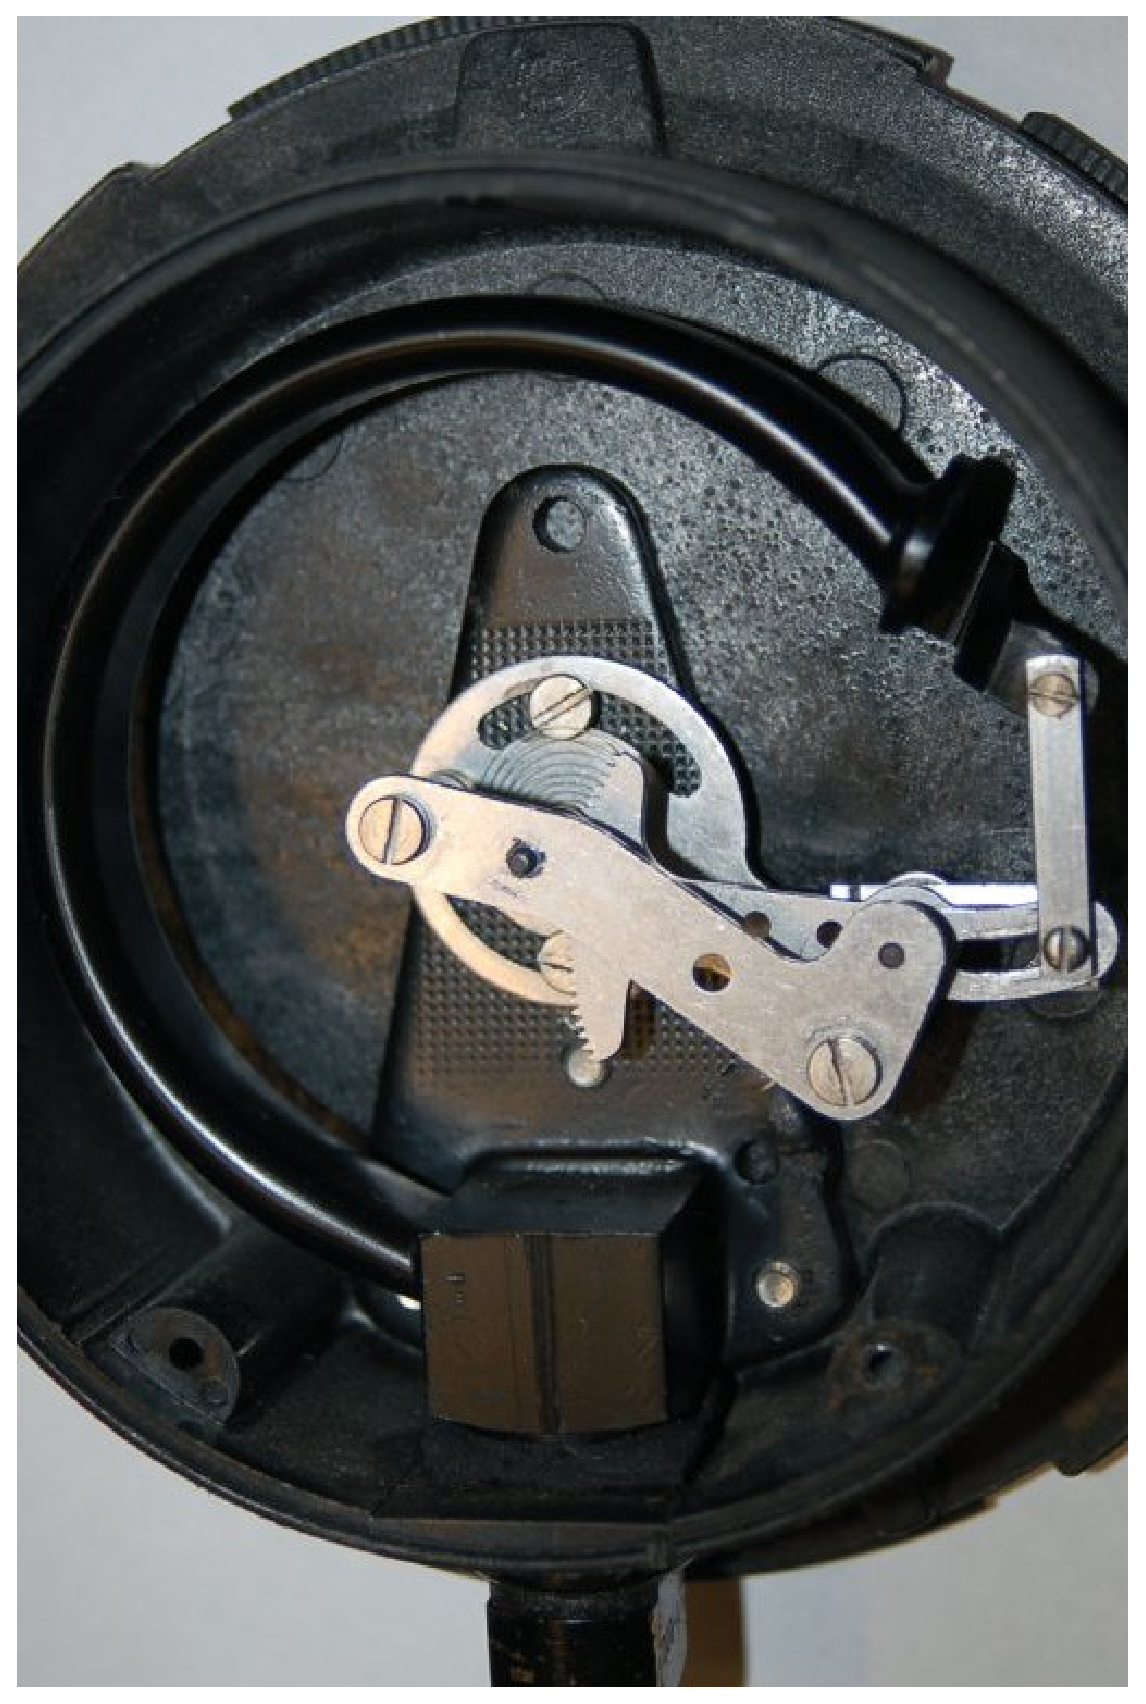
\includegraphics[height=7cm]{./bourdon_tube_closeup.eps}$$
\end{frame}

%differential and/or absolute pressure in addition to gauge pressure.  All that is needed for these other functionalities is to subject the \textit{other} side of each pressure-sensing element to either another applied pressure (in the case of differential measurement) or to a vacuum chamber (in the case of absolute pressure measurement).
%
%\filbreak
%
%This next set of illustrations shows how bellows, diaphragms, and bourdon tubes may be used as differential pressure-sensing elements:
%
%$$\includegraphics{019.eps}$$
%
%The challenge in doing this, of course, is how to extract the mechanical motion of the pressure-sensing element to an external mechanism (such as a pointer) while maintaining a good pressure seal.  In gauge pressure mechanisms, this is no problem because one side of the pressure-sensing element must be exposed to atmospheric pressure anyway, and so that side is always available for mechanical connection.
%
%A differential pressure gauge is shown in the next photograph.  The two pressure ports are clearly evident on either side of the gauge:
%
%$$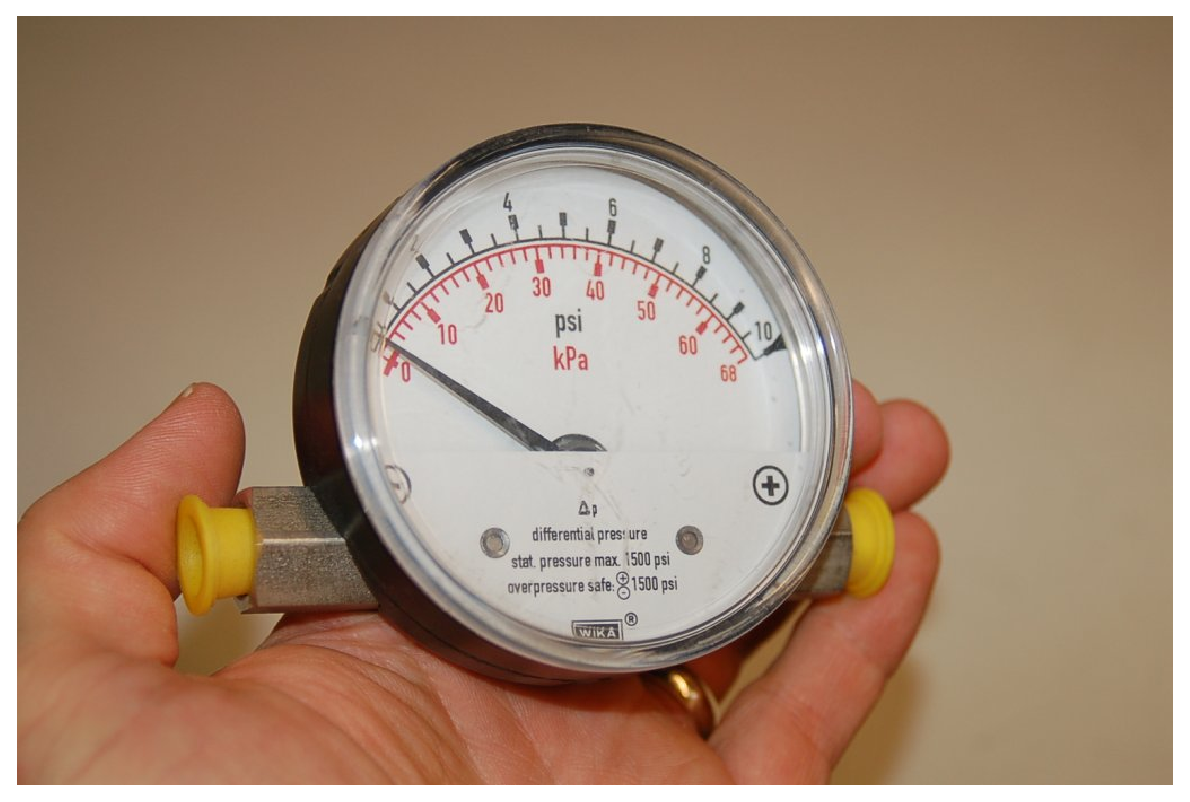
\includegraphics[width=3in]{pressure53.eps}$$
\begin{frame}
	\frametitle{Mekanisk måling av differansetrykk}

	$$\includegraphics[height=7cm]{019.eps}$$
\end{frame}

%
%
%
%
%\filbreak
%\section{Electrical pressure elements}
%
%Several different technologies exist for the conversion of fluid pressure into an electrical signal response.  These technologies form the basis of electronic \textit{pressure transmitters}: devices designed to measure fluid pressure and transmit that information via electrical signals such as the 4-20 mA analog standard, or in digital form such as HART or FOUNDATION Fieldbus.
%
%A brief survey of electronic pressure transmitters in contemporary\footnote{As of this writing, 2008.} use reveals a diverse representation of electrical pressure-sensing elements:
%
%% No blank lines allowed between lines of an \halign structure!
%% I use comments (%) instead, so Tex doesn't choke.
%
\begin{frame}
	\frametitle{Elektriske trykksensorer}


	\begin{center}
		\begin{tabular}{| c | c | c |}	
		\hline
\textbf{Fabrikant} & \textbf{Modell} & \textbf{Trykk sensor teknologi} \cr
\hline
\hline
ABB/Bailey & PTSP & Piezoresistive (strain gauge) \cr
\hline
Foxboro & IDP10 & Piezoresistive (strain gauge) \cr
\hline
Honeywell & ST3000 & Piezoresistive (strain gauge) \cr
\hline
Rosemount & 1151 & Differential capacitance \cr
\hline
Rosemount & 3051 & Differential capacitance \cr
\hline
Rosemount & 3095 & Differential capacitance \cr
\hline
	\end{tabular}
\end{center}
\end{frame}
%
%
%
%
%
%
%
%\filbreak
%\subsection{Piezoresistive (strain gauge) sensors}
%
%\textit{Piezoresistive} means ``pressure-sensitive resistance,'' or a resistance that changes value with applied pressure.  The \textit{strain gauge} is a classic example of a piezoresistive element, a typical strain gauge element shown here on the tip of my finger:  \index{Strain gauge}
%
%$$\includegraphics[width=4in]{bridge08.eps}$$
\begin{frame}
	\frametitle{Piezoresistive trykksensor}
Piezoresistive=trykk følsom resistans
	$$\includegraphics[height=7cm]{bridge08.eps}$$
\end{frame}

%
%In order to be practical, a strain gauge must be glued (\textit{bonded}) on to a larger specimen capable of withstanding an applied force (stress):
%
%$$\includegraphics{bridge05.eps}$$
\begin{frame}
	\frametitle{Målekrets med strekklapp}

	$$\includegraphics[height=7cm]{bridge05.eps}$$
\end{frame}

%
%As the test specimen is stretched or compressed by the application of force, the conductors of the strain gauge are similarly deformed.  Electrical resistance of any conductor is proportional to the ratio of length over cross-sectional area ($R \propto {l \over A}$), which means that tensile deformation (stretching) will increase electrical resistance by simultaneously increasing length and decreasing cross-sectional area while compressive deformation (squishing) will decrease electrical resistance by simultaneously decreasing length and increasing cross-sectional area.
%
%Attaching a strain gauge to a diaphragm results in a device that changes resistance with applied pressure.  Pressure forces the diaphragm to deform, which in turn causes the strain gauge to change resistance.  By measuring this change in resistance, we can infer the amount of pressure applied to the diaphragm.
%
%The classic strain gauge system represented in the previous illustration is made of metal (both the test specimen and the strain gauge itself).  Within its elastic limits, many metals exhibit good spring characteristics.  Metals, however, are subject to \textit{fatigue} over repeated cycles of strain (tension and compression), and they will begin to ``flow'' if strained beyond their elastic limit.  This is a common source of error in metallic piezoresistive pressure instruments: if overpressured, they tend to lose accuracy due to damage of the spring and strain gauge elements.\footnote{For a simple demonstration of metal fatigue and metal ``flow,'' simply take a metal paper clip and repeatedly bend it back and forth until you feel the metal wire weaken.  Gentle force applied to the paper clip will cause it to deform in such a way that it returns to its original shape when the force is removed.  Greater force, however, will exceed the paper clip's elastic limit, causing permanent deformation and also altering the spring characteristics of the clip.}  \index{Metal fatigue}
%
%Modern manufacturing techniques have made possible the construction of strain gauges made of silicon instead of metal.  Silicon exhibits very linear spring characteristics over its narrow range of motion, and a high resistance to fatigue.  When a silicon strain gauge is over-stressed, it fails completely rather than ``flows'' as is the case with metal strain gauges.  This is generally considered a better result, as it clearly indicates the need for sensor replacement (whereas a metallic strain sensor may give the false impression of continued function following an over-stress event).  \index{Silicon strain gauge element}
%
%\filbreak
%
%Thus, most modern piezoresistive-based pressure instruments use silicon strain gauge elements to sense deformation of a diaphragm due to applied fluid pressure.  A simplified illustration of a diaphragm / strain gauge pressure sensor is shown here:
%
%$$\includegraphics{pressure49.eps}$$
\begin{frame}
	\frametitle{Målekrets med strekklapp montert på mekanisk trykksensor}

	$$\includegraphics[height=7cm]{./pressure49.eps}$$
\end{frame}

%
%As the diaphragm bows outward with applied fluid pressure, the strain gauge stretches to a greater length, causing its resistance to increase.  This change in resistance imbalances the bridge circuit, causing a voltage ($V_{out}$) proportional to the amount of applied pressure.  Thus, the strain gauge works to convert an applied pressure into a measurable voltage signal which may be amplified and converted into a 4-20 mA loop current signal (or into a digital ``fieldbus'' signal).
%
%% ADD: show illustrations exaggerating the deformation of the diaphragm, both with an applied pressure and an applied vacuum
%
%\filbreak
%
%In some designs, a single silicon wafer serves as both the diaphragm and the strain gauge so as to fully exploit the excellent mechanical properties of silicon (high linearity and low fatigue).  However, silicon is not chemically compatible with many process fluids, and so pressure must be transferred to the silicon diaphragm/sensor via a non-reactive \textit{fill fluid} (commonly a silicone-based or fluorocarbon-based liquid).  A metal \textit{isolating diaphragm} transfers process fluid pressure to the fill fluid, which in turn transfers pressure to the silicon wafer.  Another simplified illustration shows how this works: \index{Isolating diaphragm} \index{Diaphragm, isolating} \index{Fill fluid}
%
%$$\includegraphics{pressure50.eps}$$
%
%The isolating diaphragm is designed to be much more flexible (less rigid) than the silicon diaphragm, because its purpose is to seamlessly transfer fluid pressure from the process fluid to the fill fluid, not to act as a spring element.  In this way, the silicon sensor experiences the same pressure that it would if it were directly exposed to the process fluid, without having to contact the process fluid.  The flexibility of the metal isolating diaphragm also means it experiences much less stress than the silicon sensing diaphragm, which avoiding the problems of metal fatigue experienced by transmitter designs using metal as the sensing (spring) element.
%
%This use of a fill fluid to transfer pressure from an isolating diaphragm to a sensing diaphragm inside the transmitter is used in most if not all modern pressure transmitter designs, even those that are not piezoresistive.
%
%\filbreak
%
%An example of a pressure instrument utilizing a silicon strain gauge element is the Foxboro model IDP10 differential pressure transmitter, shown in the following photograph:  \index{Foxboro model IDP10 differential pressure transmitter}
%
%$$\includegraphics[width=3in]{dpcell_5.eps}$$
%
%
%
%
%
%
%\filbreak
%\subsection{Differential capacitance sensors}
%
%Another common electrical pressure sensor design works on the principle of \textit{differential capacitance}.  In this design, the sensing element is a taut metal diaphragm located equidistant between two stationary metal surfaces\footnote{In the following diagram, both the sensing diaphragm and the stationary metal surfaces are shown colored blue, to distinguish these electrical elements from the other structural components of the device.}, comprising three plates for a complementary pair of capacitors.  An electrically insulating fill fluid (usually a liquid silicone compound) transfers motion from the isolating diaphragms to the sensing diaphragm, and also doubles as an effective dielectric for the two capacitors: \index{Differential capacitance pressure sensor} \index{Isolating diaphragm} \index{Diaphragm, isolating} \index{Fill fluid}
%
%$$\includegraphics{pressure31.eps}$$
\begin{frame}
	\frametitle{Kapasitive trykksensorer}

	$$\includegraphics[height=7cm]{pressure31.eps}$$
\end{frame}

%
%Any difference of pressure across the cell causes the diaphragm to flex in the direction of least pressure.  The sensing diaphragm is a precision-manufactured spring element, meaning that its displacement is a predictable function of applied force.  The applied force in this case can only be a function of differential pressure acting against the surface area of the diaphragm in accordance with the standard force-pressure-area equation $F=PA$.  In this case, we have two forces caused by two fluid pressures working against each other, so our force-pressure-area equation may be re-written to describe \textit{resultant} force as a function of differential pressure ($P_1 - P_2$) and diaphragm area: $F = (P_1 - P_2)A$.  Since diaphragm area is constant, and force is predictably related to diaphragm displacement, all we need now in order to infer differential pressure is to accurately measure displacement of the diaphragm.
%
%\filbreak
%
%The diaphragm's secondary function as one plate of two capacitors provides a convenient method for measuring displacement.  Since capacitance between conductors is inversely proportional to the distance separating them, capacitance on the low-pressure side will increase while capacitance on the high-pressure side will decrease:
%
%$$\includegraphics{pressure32.eps}$$
\begin{frame}
	\frametitle{Kapasitive trykksensorer}

	$$\includegraphics[height=7cm]{pressure32.eps}$$
\end{frame}
%
%A capacitance detector circuit connected to this cell uses a high-frequency AC excitation signal to measure the different in capacitance between the two halves, translating that into a DC signal which ultimately becomes the signal output by the instrument representing pressure.
%
%These pressure sensors are highly accurate, stable, and rugged.  An interesting feature of this design -- using two isolating diaphragms to transfer process fluid pressure to a single sensing diaphragm through an internal ``fill fluid'' -- is that the solid frame bounds the motion of the two isolating diaphragms such that neither one is able to force the sensing diaphragm past its elastic limit.  As the illustration shows, the higher-pressure isolating diaphragm gets pushed toward the metal frame, transferring its motion to the sensing diaphragm via the fill fluid.  If too much pressure is applied to that side, the isolating diaphragm will merely ``flatten'' against the solid frame of the capsule and stop moving.  This positively limits the isolating diaphragm's motion so that it cannot possibly exert any more force on the sensing diaphragm, even if additional process fluid pressure is applied.  This use of isolating diaphragms and fill fluid to transfer motion to the sensing diaphragm, employed in other styles of differential pressure sensor as well, gives modern differential pressure instruments excellent resistance to overpressure damage.
%
%It should be noted that the use of a liquid fill fluid is key to this overpressure-resistant design.  In order for the sensing diaphragm to accurately translate applied pressure into a proportional capacitance, it must not contact the conductive metal frame surrounding it.  In order for any diaphragm to be protected against overpressure, however, it must contact a solid backstop to limit further travel.  Thus, the need for non-contact (capacitance) and for contact (overpressure protection) are mutually exclusive, making it nearly impossible to perform both functions with a single sensing diaphragm.  Using fill fluid to transfer pressure from isolating diaphragms to the sensing diaphragm allows us to separate the function of capacitive measurement (sensing diaphragm) from the function of overpressure protection (isolation diaphragms) so that each diaphragm may be optimized for a separate purpose.  \index{Fill fluid}
%
%\filbreak
%
%A classic example of a pressure instrument based on the differential capacitance sensor is the Rosemount model 1151 differential pressure transmitter, shown in assembled form in the following photograph: \index{Rosemount model 1151 differential pressure transmitter}
%
%$$\includegraphics[width=5in]{diff_capacitance_1.eps}$$
%
\begin{frame}
	\frametitle{Rosemount 1151}

	$$\includegraphics[height=7cm]{diff_capacitance_1.eps}$$
\end{frame}
\begin{frame}
	\frametitle{Rosemount 1151}

	$$\includegraphics[height=7cm]{diff_capacitance_3.eps}$$
\end{frame}
\begin{frame}
	\frametitle{Rosemount 1151}

	$$\includegraphics[height=7cm]{diff_capacitance_4.eps}$$
\end{frame}
\begin{frame}
	\frametitle{Rosemount 1151}

	$$\includegraphics[height=7cm]{diff_capacitance_5.eps}$$
\end{frame}
%\filbreak
%
%By removing four bolts from the transmitter, we are able to remove two flanges from the pressure capsule, exposing the isolating diaphragms to plain view:
%
%$$\includegraphics[width=5in]{diff_capacitance_3.eps}$$
%
%A close-up photograph shows the construction of one of the isolating diaphragms, which unlike the sensing diaphragm is designed to be very flexible.  The concentric corrugations in the metal of the diaphragm allow it to easily flex with applied pressure, transmitting process fluid pressure through the silicone fill fluid to the taut sensing diaphragm inside the differential capacitance cell: \index{Isolating diaphragm} \index{Diaphragm, isolating} \index{Fill fluid}
%
%$$\includegraphics[width=4in]{diff_capacitance_4.eps}$$
%
%\filbreak
%
%The interior of the same differential capacitance sensor (revealed by cutting a Rosemount model 1151 sensor in half with a chop saw\footnote{A chop saw is admittedly not a tool of finesse, and it did a fair job of mangling this unfortunate differential capacitance cell.  A bandsaw was tried at first, but made virtually no progress in cutting the hard stainless steel of the capsule assembly.  The chop saw's abrasive wheel created a lot of heat, discoloring the metal and turning the silicone fill fluid into a crystalline mass which had to be carefully chipped out by hand using an ice pick so as to not damage the thin metal sensing diaphragm.  Keep these labors in mind, dear reader, as you enjoy this textbook!}) shows the isolating diaphragms, the sensing diaphragm, and the ports connecting them together:
%
%$$\includegraphics[width=4in]{diff_capacitance_5.eps}$$
%
%Here, the left-side isolating diaphragm is clearer to see than the right-side isolating diaphragm.  A feature clearly evident in this photograph is the small clearance between the left-side isolating diaphragm and the internal metal frame, versus the spacious chamber in which the sensing diaphragm resides.  Recall that these internal spaces are normally occupied by \textit{fill fluid}, the purpose of which is to transfer pressure from the isolating diaphragms to the sensing diaphragm.  As mentioned before, the solid metal frame limits the travel of each isolating diaphragm in such a way that the higher-pressure isolating diaphragm ``bottoms out'' on the metal frame before the sensing diaphragm can be pushed past its elastic limit.  In this way, the sensing diaphragm is protected against damage from overpressure because the isolating diaphragms are simply not allowed to move any farther.
%
%\vskip 10pt
%
%\filbreak
%
%The differential capacitance sensor inherently measures \textit{differences} in pressure applied between its two sides.  In keeping with this functionality, this pressure instrument has two threaded ports into which fluid pressure may be applied.  A later section in this chapter will elaborate on the utility of differential pressure transmitters (section \ref{Differential pressure transmitters} beginning on page \pageref{Differential pressure transmitters}).  All the electronic circuitry necessary for converting the sensor's differential capacitance into an electronic signal representing pressure is housed in the blue-colored structure above the capsule and flanges.
%
%% ADD: refer to "Principles of Applied Biomedical Instrumentation" pages 72-73 discussing the Twin-T Capacitive transducer circuit, and also the Rosemount 1151 analog schematic, if I can make sense of it.
%
%\vskip 10pt
%
%\filbreak
%
%A more modern realization of the differential capacitance pressure-sensing principle is the Rosemount model 3051 differential pressure transmitter: \index{Rosemount model 3051 differential pressure transmitter}
%
%$$\includegraphics[width=5in]{diff_capacitance_2.eps}$$
\begin{frame}
	\frametitle{Rosemount 3051}

	$$\includegraphics[height=7cm]{diff_capacitance_2.eps}$$
\end{frame}
%
%As is the case with all differential pressure devices, this instrument has \textit{two} ports through which fluid pressure may be applied to the sensor.  The sensor, in turn, responds only to the \textit{difference} in pressure between the ports.
%
%\filbreak
%
%The differential capacitance sensor construction is more complex in this particular pressure instrument, with the plane of the sensing diaphragm perpendicular to the plane of the two isolating diaphragms.  This ``coplanar'' design is more compact than the older style of sensor, and more importantly it isolates the sensing diaphragm from flange bolt stress -- one of the main sources of error in the previous design\footnote{Not only did applied torque of the four capsule bolts affect measurement accuracy in the older 1151 model design, but changes in temperature resulting in changing bolt tension also had a detrimental impact on accuracy.  Most modern differential pressure transmitter designs strive to isolate the sensing diaphragm assembly from flange bolt stress for these reasons.}.  \index{Coplanar DP sensor}
%
%$$\includegraphics{pressure71.eps}$$
\begin{frame}
	\frametitle{Rosemount 3051}

	$$\includegraphics[height=7cm]{pressure71.eps}$$
\end{frame}
%
%Take particular note of how the sensor assembly is not embedded in the solid metal frame as was the case with the original Rosemount design.  Instead, the sensor assembly is relatively isolated from the frame, connected only by two capillary tubes joining it to the isolating diaphragms.  This way, stresses inside the metal frame imparted by flange bolts have virtually no effect on the sensor.
%
%\filbreak
%
%A cutaway model of a Rosemount model 3051S (``supermodule'') DP transmitter shows how this all looks in real life:  \index{Rosemount model 3051S differential pressure transmitter}
%
%$$\includegraphics[width=5in]{diff_capacitance_6.eps}$$
\begin{frame}
	\frametitle{Rosemount 3051}

	$$\includegraphics[height=7cm]{diff_capacitance_6.eps}$$
\end{frame}
%
%Process fluid pressure applied to the isolating diaphragm(s) transfers to fill fluid inside the capillary tubes, conveying pressure to the taut diaphragm inside the differential capacitance sensor.  Like the classic Rosemount model 1151 design, we see the fill fluid performing multiple functions: 
%
%\begin{itemize}
%\item The fill fluid protects the delicate sensing diaphragm from contact with unclean or corrosive process fluids
%\item The fill fluid allows the isolating diaphragms to provide overpressure protection for the sensing diaphragm
%\item The fill fluid provides a medium of constant permittivity for the differential capacitance circuit to function
%\end{itemize}
%
%The ``supermodule'' series of Rosemount pressure transmitters shares the same coplanar design as the earlier 3051 models, but adds a new design feature: inclusion of the electronics within the stainless-steel module rather than the blue-painted upper housing.  This feature allows the transmitter size to be significantly reduced if needed for applications with limited space.
%
%
%
%
%
%
%
%%\filbreak
%%\subsection{Differential reluctance sensor}
%
%% ADD: ABB/Bailey "Platinum series" PTSD differential pressure transmitters
%
%
%
%
%
%
%
%
%
%\filbreak
%\subsection{Resonant element sensors}
%
%As any guitarist, violinist, or other stringed-instrument musician can tell you, the natural frequency of a tensed string increases with tension.  This, in fact, is how stringed instruments are tuned: the tension on each string is precisely adjusted to achieve the desired resonant frequency.
%
%Mathematically, the resonant frequency of a string may be described by the following formula:
%
%$$f = {1 \over 2L} \sqrt{F_T \over \mu}$$
%
%\noindent
%Where,
%
%$f$ = Fundamental resonant frequency of string (Hertz)
%
%$L$ = String length (meters)
%
%$F_T$ = String tension (newtons)
%
%$\mu$ = Unit mass of string (kilograms per meter)
%
%\vskip 10pt
%
%It stands to reason, then, that a string may serve as a force sensor.  All that is needed to complete the sensor is an oscillator circuit to keep the string vibrating at its resonant frequency, and that frequency becomes an indication of tension (force).  If the force originates from pressure applied to some sensing element such as a bellows or diaphragm, the string's resonant frequency will indicate fluid pressure.  A proof-of-concept device based on this principle might look like this:
%
%$$\includegraphics{pressure43.eps}$$
%
%It should be noted that this principle of force measurement is nonlinear\footnote{For example, a doubling of force results in a frequency increase of 1.414 (precisely equal to $\sqrt{2}$).  A \textit{four}-fold increase in pressure would be necessary to \textit{double} the string's resonant frequency.  This particular form of nonlinearity, where diminishing returns are realized as the applied stimulus increases, yields excellent rangeability.  In other words, the instrument is inherently more sensitive to changes in pressure at the low end of its sensing range, and ``de-sensitizes'' itself toward the high end of its sensing range.}, as indicated by the equation for resonant frequency (tension force $F$ lies inside the radicand).  This means the pressure transmitter must be designed with an electronic characterizing function to ``linearize'' the frequency measurement into a pressure measurement.
%
%\filbreak
%
%The Foxboro company pioneered this concept in an early \textit{resonant wire} design of pressure transmitter.  Later, the Yokogawa corporation of Japan applied the concept using a pair of micro-machined\footnote{This is an example of a micro-electro-mechanical system, or \textit{MEMS}.} silicon resonator structures bonded to a single sensing diaphragm, which became the basis for their successful line of ``DPharp'' pressure transmitters.  \index{Resonant wire pressure sensor}  \index{Yokogawa DPharp pressure transmitter} \index{Silicon resonator pressure sensor}  \index{MEMS} 
%
%A photograph of a Yokogawa model EJA110 pressure transmitter with this technology is seen here:  \index{Yokogawa model EJA110 differential pressure transmitter}
%
%$$\includegraphics[width=3in]{yokogawa_dpharp_1.eps}$$
%
%Process pressure enters through ports in two flanges, presses against a pair of isolating diaphragms, transferring motion to a single sensing diaphragm via fill fluid where the resonant elements change frequency with diaphragm strain.  Motion of the sensing diaphragm in either direction tenses one resonant element and compresses the other, causing their frequencies to deviate from each other.  Electronic circuits within the upper housing measure the two resonant elements' frequencies and generate an output signal proportional to their frequency difference.  This, of course, is a representation of applied differential pressure.  \index{Fill fluid}
%
%\filbreak
%
%Even when disassembled, the transmitter does not look much different from the more common differential capacitance sensor design.  
%
%$$\includegraphics[width=4in]{yokogawa_dpharp_2.eps}$$
%
%The important design differences are hidden from view, inside the sensing capsule.  Functionally, though, this transmitter is much the same as its differential-capacitance and piezoresistive cousins.  This design even uses fill fluid to protect the delicate silicon resonators from potentially destructive process fluids, just like differential capacitance sensors and most piezoresistive sensor designs.
%
%An interesting advantage of the resonant element pressure sensor is that the sensor signal is easily digitized.  The vibration of each resonant element is sensed by the electronics package as an AC frequency.  This frequency signal is ``counted'' by a digital counter circuit over a given span of time and converted to a binary digital representation without any need for an analog-to-digital converter (ADC) circuit.  Quartz crystal electronic oscillators are extremely precise, providing the stable frequency reference necessary for comparison in any frequency-based instrument.
%
%In the Yokogawa ``DPharp'' design, the two resonant elements oscillate at a nominal frequency of approximately 90 kHz.  As the sensing diaphragm deforms with applied differential pressure, one resonator experiences tension while the other experiences compression, causing the frequency of the former to shift up and the latter to shift down (as much as $\pm$ 20 kHz).  The signal conditioning electronics inside the transmitter measures this difference in resonator frequency to infer applied pressure.
%
%
%
%
%
%\filbreak
%\subsection{Mechanical adaptations}
%
%Most modern electronic pressure sensors convert very small diaphragm motions into electrical signals through the use of sensitive motion-sensing techniques (strain gauge sensors, differential capacitance cells, etc.).  Diaphragms made from elastic materials behave as springs, but circular diaphragms exhibit very nonlinear behavior when significantly stretched unlike classic spring designs such as coil and leaf springs which exhibit linear behavior over a wide range of motion.  Therefore, in order to yield a linear response to pressure, a diaphragm-based pressure sensor must be designed in such a way that the diaphragm stretches very little over the normal range of operation.  Limiting the displacement of a diaphragm necessitates highly sensitive motion-detection techniques such as strain gauge sensors, differential capacitance cells, and mechanical resonance sensors to convert that diaphragm's very slight motion into an electronic signal.
%
%An alternative approach to electronic pressure measurement is to use mechanical pressure-sensing elements with more linear pressure-displacement characteristics -- such as bourdon tubes and spring-loaded bellows -- and then detect the large-scale motion of the pressure element using a less-sophisticated electrical motion-sensing device such as a potentiometer, LVDT, or Hall Effect sensor.  In other words, we take the sort of mechanism commonly found in a direct-reading pressure gauge and attach it to a potentiometer (or similar device) to derive an electrical signal from the pressure measurement. \index{LVDT} \index{Hall Effect sensor}
%
%The following photographs show front and rear views of an electronic pressure transmitter using a large C-shaped bourdon tube as the sensing element (seen in the left-hand photograph):
%
%$$\includegraphics[width=2.5in]{pressure55.eps} \hskip 30pt \includegraphics[width=2.5in]{pressure56.eps}$$
%
%This alternative approach is undeniably simpler and less expensive to manufacture than the more sophisticated approaches used with diaphragm-based pressure instruments, but is prone to greater inaccuracies.  Even bourdon tubes and bellows are not perfectly linear spring elements, and the substantial motions involved with using such pressure elements introduces the possibility of hysteresis errors (where the instrument does not respond accurately during reversals of pressure, where the mechanism changes direction of motion) due to mechanism friction, and deadband errors due to backlash (looseness) in mechanical connections.
%
%You are likely to encounter this sort of pressure instrument design in direct-reading gauges equipped with electronic transmitting capability.  An instrument manufacturer will take a proven product line of pressure gauge and add a motion-sensing device to it that generates an electric signal proportional to mechanical movement inside the gauge, resulting in an inexpensive pressure transmitter that happens to double as a direct-reading pressure gauge.
%
%
%
%
%
%% \filbreak
%% \subsection{Electronic vacuum sensors}
%
%% ADD: Pirani and ionization gauges
%
%
%
%
%
%
%
%
%
%\filbreak
%\section{Differential pressure transmitters}
%
%\label{Differential pressure transmitters}
%
%One of the most common, and most useful, pressure measuring instruments in industry is the \textit{differential pressure transmitter}.  This device senses the difference in pressure between two ports and outputs a signal representing that pressure in relation to a calibrated range.  Differential pressure transmitters may be based on any of the previously discussed pressure-sensing technologies, so this section focuses on application rather than theory.
%
%
%
%
%
%
%
%\filbreak
%\subsection{DP transmitter construction and behavior}
%
%Differential pressure transmitters constructed for industrial measurement applications typically consist of a strong (forged metal) body housing the sensing element(s), topped by a compartment housing the mechanical and/or electronic components necessary to translate the sensed pressure into a standard instrumentation signal (e.g. 3-15 PSI, 4-20 mA, digital fieldbus codes):
%
%$$\includegraphics{pressure23.eps}$$
\begin{frame}
	\frametitle{DP-cellen}

	$$\includegraphics[width=1\textwidth]{pressure23.eps}$$
\end{frame}

%
%Two models of electronic differential pressure transmitter appear in the following photographs, the Rosemount model 1151 (left) and model 3051 (right):  \index{Rosemount model 1151 differential pressure transmitter}  \index{Rosemount model 3051 differential pressure transmitter}
%
%$$\includegraphics[width=2.5in]{dpcell_1.eps} \hskip 30pt \includegraphics[width=2.5in]{dpcell_2.eps}$$
\begin{frame}
	\frametitle{DP-cellen}

%	$$\includegraphics[height=7cm]{cont01.eps}$$
$$\includegraphics[width=2.5in]{dpcell_1.eps} \hskip 30pt \includegraphics[width=2.5in]{dpcell_2.eps}$$
\end{frame}

%
%\filbreak
%
%Two more models of electronic differential pressure transmitter are shown in the next photograph, the Yokogawa EJA110 (left) and the Foxboro IDP10 (right):  \index{Yokogawa model EJA110 differential pressure transmitter}  \index{Foxboro model IDP10 differential pressure transmitter}
%
%$$\includegraphics[width=1.5in]{yokogawa_dpharp_1.eps} \hskip 30pt \includegraphics[width=1.5in]{dpcell_5.eps}$$
%
%In each of these differential pressure transmitter examples, the pressure-sensing element is housed in the bottom half of the device (the forged-steel structure) while the electronics are housed in the top half (the colored, round, cast-aluminum structure).  
%
%Regardless of make or model, every differential pressure (``DP'', ``d/p'', or $\Delta$P)\footnote{As far as I have been able to determine, the labels ``D/P'' and ``DP cell'' were originally trademarks of the Foxboro Company.  Those particular transmitter models became so popular that the term ``DP cell'' came to be applied to nearly \textit{all} makes and models of differential pressure transmitter, much like the trademark ``Vise-Grip'' is often used to describe \textit{any} self-locking pliers, or ``Band-Aid'' is often used to describe \textit{any} form of self-adhesive bandage.} transmitter has \textit{two} pressure ports to sense different process fluid pressures.  These ports typically have $1 \over 4$ inch female NPT threads for convenient connection to the process.  One of these ports is labeled ``high'' and the other is labeled ``low''.  This labeling does not necessarily mean that the ``high'' port must always be at a greater pressure than the ``low'' port.  What these labels represent is the effect any increasing fluid pressure applied to that port will have on the \textit{direction} of the output signal's change.
%
%$$\includegraphics[width=4in]{pressure66.eps}$$
\begin{frame}
	\frametitle{DP-cellens H port og L port}

	$$\includegraphics[width=1\textwidth]{pressure66.eps}$$
\end{frame}

%
%\filbreak
%
%The most common sensing element used by modern DP transmitters is the diaphragm.  One side of this diaphragm receives process fluid pressure from the ``high'' port, while the other receives process fluid pressure from the ``low'' port.  Any difference of pressure between the two ports causes the diaphragm to flex from its normal resting (center) position.  This flexing is then translated into an output signal by any number of different technologies, depending on the manufacturer and model of the transmitter:
%
%$$\includegraphics{pressure65.eps}$$
\begin{frame}
	\frametitle{DP-cellens H port og L port}

	$$\includegraphics[width=1\textwidth]{pressure65.eps}$$
\end{frame}
%
%\filbreak
%
%The concept of differential pressure instrument port labeling is very similar to the ``inverting'' and ``noninverting'' labels applied to operational amplifier input terminals:
%
%$$\includegraphics{pressure24.eps}$$
%
%The ``+'' and ``$-$'' symbols do not imply polarity of the input voltage(s); i.e. it is not as though the ``+'' input must be more positive than the ``$-$'' input.  These symbols merely represent the different direction each input tends to drive the output signal.  An increasing potential applied to the ``+'' input drives the opamp's output positive, while an increasing potential applied to the ``$-$'' input drives the opamp's output negative.  Phrasing this in terms common to closed-loop control systems, we could say that the ``+'' input is \textit{direct-acting} while the ``$-$'' input is \textit{reverse-acting}.
%
%\filbreak
%
%Similarly, the ``H'' and ``L'' labels on a DP transmitter's ports do not imply magnitude of input pressures; i.e. it is not as though the ``H'' port's pressure must be greater than the ``L'' port's pressure.  These symbols merely represent the different effects on the output signal resulting from pressure applied to each port.  An increasing pressure applied to the ``high'' port of a DP transmitter will drive the output signal to a greater level (up), while an increasing pressure applied to the ``low'' port of a DP transmitter will drive the output signal to a lesser level (down)\footnote{One transmitter manufacturer I am aware of (ABB/Bailey) actually does use the ``+'' and ``$-$'' labels to denote high- and low-pressure ports rather than the more customary ``H'' and ``L'' labels found on other manufacturers' DP products.}:
%
%$$\includegraphics{pressure25.eps}$$
\begin{frame}
	\frametitle{DP-cellens H port og L port}

	$$\includegraphics[width=1\textwidth]{pressure25.eps}$$
\end{frame}
%
%The ability to arbitrarily connect a DP transmitter to a process in such a way that it is either direct-acting or reverse-acting is a great advantage, as we will later see.
%
%\vskip 10pt
%
%In the world of electronics, we refer to the ability of a differential voltage sensor (such as an operational amplifier) to sense small differences in voltage while ignoring large potentials measured with reference to ground by the phrase \textit{common-mode rejection}.  An ideal operational amplifier completely ignores the amount of voltage common to both input terminals, responding only to the \textit{difference} in voltage \textit{between} those terminals.  This is precisely what a well-designed DP instrument does, except with fluid pressure instead of electrical voltage.  A DP instrument ignores gauge pressure common to both ports, while responding only to \textit{differences} in pressure \textit{between} those two ports.  Stated in other words, a differential pressure instrument (ideally\footnote{Perfect common-mode rejection is impossible for differential pressure instruments just as it is impossible for electronic voltage-measuring instruments, but in either case the effect is usually minimal.  For differential pressure transmitters, the effect of common-mode pressure on the instrument's output signal is sometimes referred to as the \textit{line pressure effect} or \textit{static pressure effect}, typically stated as a percentage of the instrument's upper range limit per unit of common-mode pressure.}) responds only to differential pressure while ignoring common-mode pressure.  \index{Common-mode rejection}  \index{Line pressure effect, pressure transmitter}  \index{Static pressure effect, pressure transmitter}
%
%\filbreak
%
%To illustrate, we may connect the ``high'' and ``low'' ports of a differential pressure transmitter together using pipe or tube, then expose both ports simultaneously to a source of fluid pressure such as pressurized air from an air compressor.  If the transmitter is in good working order, it should continue to register zero differential pressure even as we vary the amount of static pressure applied to both ports.  So long as the applied pressures to each port are equal, the transmitter's sensing diaphragm should experience zero net force pushing left or right.  All force applied to the diaphragm from the ``high'' port's fluid pressure should be precisely countered (canceled) by force applied to the diaphragm from the ``low'' port's fluid pressure.  
%
%An electrical analogy to this would be connecting both red and black test leads of a voltmeter to a common point in an electrical circuit, then varying the amount of voltage between that point and earth ground.  Since the voltmeter only registers \textit{differences} of potential between its test leads, and those test leads are now electrically common to one another, the magnitude of common-mode voltage between that one point of the circuit and earth ground is irrelevant from the perspective of the voltmeter:
%
%$$\includegraphics{pressure57.eps}$$
%
%In each case the differential measurement device \textit{rejects} the common-mode value, registering only the amount of difference (zero) between its sensing points.
%
%\filbreak
%
%The same common-mode rejection principle reveals itself in more complex fluid and electrical circuits.  Consider the case of a DP transmitter and a voltmeter, both used to measure differential quantities in a ``divider'' circuit\footnote{The electrical circuit shown on the right uses a pair of series-connected resistors to divide the source voltage into two parts, 5 volts and 95 volts.  The pneumatic circuit shown on the left uses a pair of series-connected hand valves to divide the source pressure into two parts, 5 PSI and 95 PSI.}:
%
%$$\includegraphics{pressure58.eps}$$
%
%In each case the differential measurement device responds only to the difference between the two measurement points, rejecting the common-mode value (97.5 PSI for the pressure transmitter, 97.5 volts for the voltmeter).  Just to make things interesting in this example, the ``high'' side of each measuring instrument connects to the point of lesser value, such that the measured difference is a negative quantity.  Like digital voltmeters, modern DP transmitters are equally capable of accurately measuring negative pressure differences as well as positive pressure differences.
%
%\filbreak
%
%A vivid contrast between \textit{differential} pressure and \textit{common-mode} pressure for a DP instrument is seen in the pressure ratings shown on the nameplate of a Foxboro model 13A differential pressure transmitter:
%
%$$\includegraphics[width=5in]{dpcell_6.eps}$$
%
%This nameplate tells us that the transmitter has a calibrated differential pressure range of 50" H$_{2}$O (50 inches water column, which is only about 1.8 PSI).  However, the nameplate also tells us that the transmitter has a \textit{maximum working pressure} (MWP) of 1500 PSI.  ``Working pressure'' refers to the amount of gauge pressure common to each port, not the differential pressure between ports.  Taking these figures at face value means this transmitter will register zero (no differential pressure) even if the gauge pressure applied equally to both ports is a full 1500 PSI!  In other words, this differential pressure transmitter will \textit{reject} up to 1500 PSI of common-mode gauge pressure, and respond only to small differences in pressure between the ports (1.8 PSI differential being enough to stimulate the transmitter to full scale output). \index{Maximum working pressure} \index{MWP}
%
%
%
%
%
%
%
%
%
%\filbreak
%\subsection{DP transmitter applications}
%
%The combination of two differential pressure ports makes the DP transmitter very versatile as a pressure-measuring device.  This one instrument may be used to measure pressure differences, positive (gauge) pressures, negative (vacuum) pressures, and even absolute pressures, just by connecting the ``high'' and ``low'' sensing ports differently.
%
%In every DP transmitter application, there must be some means of connecting the transmitter's pressure-sensing ports to the points in a process.  Metal or plastic tubes (or pipes) work well for this purpose, and are commonly called \textit{impulse lines}, or \textit{gauge lines}, or \textit{sensing lines}\footnote{Also called impulse \textit{tubes}, gauge \textit{tubes}, or sensing \textit{tubes}.}.  This is equivalent to the test wires used to connect a voltmeter to points in a circuit for measuring voltage.  Typically, these tubes are connected to the transmitter and to the process by means of \textit{compression fittings} which allow for relatively easy disconnection and reconnection of tubes.  For more information on instrument tube fittings, refer to section \ref{Compression_tube_fittings} beginning on page \pageref{Compression_tube_fittings}.  \index{Impulse line} \index{Impulse tube} \index{Gauge line} \index{Gauge tube} \index{Sensing line} \index{Sensing tube} \index{Compression fitting}
%
%
%
%
%
%
%\filbreak
%\subsubsection{Measuring process vessel clogging}
%
%We may use the DP transmitter to measure an actual difference of pressure across a process vessel such as a filter, a heat exchanger, or a chemical reactor.  The following illustration shows how a differential pressure transmitter may be used to measure clogging of a water filter:
%
%$$\includegraphics{pressure26.eps}$$
\begin{frame}
	\frametitle{Måle om prosessutstyr er tett}

	$$\includegraphics[height=7cm]{pressure26.eps}$$
\end{frame}

%
%Note how the high side of the DP transmitter connects to the upstream side of the filter, and the low side of the transmitter to the downstream side of the filter.  This way, increased filter clogging will result in an increased transmitter output.  Since the transmitter's internal pressure-sensing diaphragm only responds to \textit{differences} in pressure between the ``high'' and ``low'' ports, the pressure in the filter and pipe relative to the atmosphere is completely irrelevant to the transmitter's output signal.  The filter could be operating at a line pressure of 10 PSI or 10000 PSI -- the only variable the DP transmitter measures is the pressure \textit{drop} across the filter.  If the upstream side is at 10 PSI and the downstream side is at 9 PSI, the differential pressure will be 1 PSI (sometimes labeled as PSID, ``D'' for \textit{differential}).  If the upstream pressure is 10000 PSI and the downstream pressure is 9999 PSI, the DP transmitter will still see a differential pressure of just 1 PSID.  Likewise, the technician calibrating the DP transmitter on the workbench could use a precise air pressure of just 1 PSI (applied to the ``high'' port, with the ``low'' port vented to atmosphere) to simulate either of these real-world conditions.  The DP transmitter simply cannot tell the difference between these three scenarios, nor should it be able to tell the difference if its purpose is to exclusively measure differential pressure.
%
%
%
%
%
%
%\filbreak
%\subsubsection{Measuring positive gauge pressure}
%
%DP instruments may also serve as simple \textit{gauge pressure} instruments if needed, responding to pressures in excess of atmosphere.  If we simply connect the ``high'' side of a DP instrument to a process vessel using an impulse tube, while leaving the ``low'' side vented to atmosphere, the instrument will interpret any positive pressure in the vessel as a positive \textit{difference} between the vessel and atmosphere:
%
%$$\includegraphics{pressure59.eps}$$
\begin{frame}
	\frametitle{Måling av overtykk i tanker}

	$$\includegraphics[height=7cm]{pressure59.eps}$$
\end{frame}
%
%Although this may seem like a waste of the transmitter's abilities (why not just use a simpler gauge pressure transmitter with just one port?), it is actually a very common application for DP transmitters.  This usage of a differential device may not actually be a ``waste'' if true-differential applications exist at the same facility for that pressure transmitter, which means only one spare transmitter need be stocked in the facility's warehouse instead of two spare transmitters (one of each type).
%
%\vskip 10pt
%
%\filbreak
%
%Most DP instrument manufacturers offer ``gauge pressure'' versions of their differential instruments, with the ``high'' side port open for connection to an impulse line and the ``low'' side of the sensing element capped off with a special vented flange, effectively performing the same function we see in the above example at a slightly lesser cost.  A close-up photograph of a Rosemount model 1151GP gauge pressure transmitter shows the port-less flange on the ``low'' side of the pressure-sensing module.  Only the ``high'' side of the sensor has a place for an impulse line to connect:
%
%$$\includegraphics[width=4in]{dpcell_7.eps}$$
\begin{frame}
	\frametitle{Måling av gauge trykk}

	$$\includegraphics[height=7cm]{dpcell_7.eps}$$
\end{frame}

%
%\filbreak
%
%A closer look at this flange reveals a vent near the bottom, ensuring the ``low'' side of the pressure-sensing capsule always senses ambient (atmospheric) pressure:
%
%$$\includegraphics[width=4in]{dpcell_8.eps}$$
\begin{frame}
	\frametitle{Måling av gauge trykk}

	$$\includegraphics[height=7cm]{dpcell_8.eps}$$
\end{frame}
%
%
%
%
%\filbreak
%\subsubsection{Measuring absolute pressure}
%
%Absolute pressure is defined as the difference between a given fluid pressure and a perfect vacuum, as opposed to gauge pressure which is the difference between a fluid's pressure and the atmospheric air pressure.  We may build an absolute pressure sensing instrument by taking a DP instrument and sealing the ``low'' side of its pressure-sensing element in connection to a vacuum chamber.  This way, any pressure greater than a perfect vacuum will register as a positive difference:
%
%$$\includegraphics{pressure61.eps}$$
\begin{frame}
	\frametitle{Måling av absolutt trykk}

	$$\includegraphics[width=1\textwidth]{pressure61.eps}$$
\end{frame}

%
%Most absolute pressure transmitters resemble ``gauge pressure'' adaptations of DP transmitters, with only one port available to connect an impulse line.  Unlike gauge pressure transmitters, though, absolute pressure transmitters do \textit{not} have vent holes on their ``low'' sides.  The ``low'' side of an absolute pressure transmitter must be a sealed vacuum in order to accurately measure the ``high'' side fluid pressure in absolute terms.
%
%\vskip 10pt
%
%Absolute pressure measurement is important for a variety of process applications, including boiling-point control and mass flow measurement of gases.  The boiling temperature of any liquid is a function of the absolute pressure it experiences, and in applications where boiling temperature must be precisely controlled in order to achieve a certain outcome (e.g. vacuum distillation of crude oil, for example) the best type of pressure measurement to use absolute.  When computing the mass flow rate of gases in a pipe, the relationship between volume and molecular count is a function of both temperature and pressure (both absolute), and so absolute pressure measurement is indispensable here as well.
%
%
%
%
%
%\filbreak
%\subsubsection{Measuring vacuum}
%
%The same principle of connecting one port of a DP device to a process and venting the other works well as a means of measuring \textit{vacuum} (pressures below that of atmosphere).  All we need to do is connect the ``low'' side to the vacuum process and vent the ``high'' side to atmosphere:
%
%$$\includegraphics{pressure60.eps}$$
\begin{frame}
	\frametitle{Måling av vakum}

	$$\includegraphics[height=7cm]{pressure60.eps}$$
\end{frame}

%
%Any pressure in the process vessel less than atmospheric will register to the DP transmitter as a \textit{positive} difference (with $P_{high}$ greater than $P_{low}$).  Thus, the stronger the vacuum in the process vessel, the greater the signal output by the transmitter.
%
%This last statement deserves some qualification.  It used to be, the way analog pneumatic and electronic transmitters were designed many years ago, that the only way to obtain an increasing signal from a DP instrument was to ensure the ``high'' port pressure \textit{rose} in relation to the ``low'' port pressure (or conversely stated, to ensure the ``low'' port pressure \textit{dropped} in relation to the ``high'' side pressure).  However, with the advent of digital electronic technology, it became rather easy to program a DP instrument with a \textit{negative} range, for example 0 to $-10$ PSI.  This way, a \textit{decreasing} pressure as interpreted by the transmitter would yield an \textit{increasing} output signal.
%
%It is rare to find a pressure transmitter calibrated in such a way, but bear in mind that it is possible.  This opens the possibility of using a regular ``gauge'' pressure transmitter (where the ``high'' port connects to the process vessel and the ``low'' port is always vented to atmosphere by virtue of a special flange on the instrument) as a vacuum instrument.  If a gauge pressure transmitter is given a negative calibration span, any decreasing pressure seen at the ``high'' port will yield an increasing output signal.
%
%
%
%
%
%\filbreak
%\subsection{Inferential measurement applications}
%
%A very common technique in industrial instrumentation is to calculate the value of a process variable from the values of related variables which are easier to measure\footnote{Truth be told, \textit{most} process variables are inferred rather than directly measured.  Even pressure, which is being used here to infer measurements such as liquid level and fluid flow, is itself inferred from some other variable inside the DP instrument (e.g. capacitance, strain gauge resistance, resonant frequency)!}.  As it so happens, there are a host of variables which one may infer from readings of differential pressure.  This makes DP transmitters very versatile devices, not just limited to measuring process variables of pressure and vacuum.  This portion of the book will explore some of the more common inferred measurements possible with DP instruments.
%
%
%
%
%
%
%\filbreak
%\subsubsection{Inferring liquid level}
%
%Liquids generate pressure proportional to height (depth) due to their weight.  The pressure generated by a vertical column of liquid is proportional to the column height ($h$), and liquid's mass density ($\rho$), and the acceleration of gravity ($g$):
%
%$$P = \rho g h$$
%
%Knowing this, we may use a DP transmitter as a liquid level-sensing device if we know the density of the liquid remains fairly constant\footnote{We simply assume Earth's gravitational acceleration ($g$) to be constant as well.}:
%
%$$\includegraphics{pressure62.eps}$$
\begin{frame}
	\frametitle{Indirekte måling av nivå}

	$$\includegraphics[height=6cm]{pressure62.eps}$$
$$P = \rho g h \Rightarrow h = {P \over {\rho g}}$$
\end{frame}

%
%As liquid level in the vessel increases, the amount of hydrostatic pressure applied to the transmitter's ``high'' port increases in direct proportion.  The width of the vessel is irrelevant to the amount of pressure produced -- only the liquid \textit{height} ($h$), \textit{density} ($\rho$), and Earth's gravity ($g$) are significant.  Thus, the transmitter's increasing signal represents the height of liquid inside the vessel, no matter the size or shape of the vessel:
%
%$$h = {P \over {\rho g}}$$
%
%\filbreak
%
%This simple technique works even if the vessel is under pressure from a gas or a vapor (rather than being vented as was the case in the previous example).  All we need to do to compensate for this other pressure is to connect the DP transmitter's ``low'' port to the top of the vessel so it senses nothing but the gas pressure:
%
%$$\includegraphics{pressure63.eps}$$
\begin{frame}
	\frametitle{Indirekte måling av nivå}

	$$\includegraphics[height=6cm]{pressure63.eps}$$
$$P = \rho g h \Rightarrow h = {P \over {\rho g}}$$
\end{frame}
%
%Since the transmitter responds only to differences of pressure between its two sensing ports, and the only cause for a difference of pressure in this application will be pressure generated by the height of a liquid column, the transmitter's signal becomes an exclusive representation of liquid level in the vessel, rejecting potential measurement errors caused by changes in gas pressure within the vessel.  Any gas pressure within the vessel will be sensed equally by both ports on the transmitter as a ``common-mode'' pressure, thus canceling each other and having no effect on the differential pressure measurement.  Only changes in liquid level within the vessel will cause the ``high'' port pressure to change independently of the ``low'' port pressure, changing the transmitter's output signal.
%
%
%%\filbreak
%%\subsubsection{Inferring liquid density}
%
%
%
%
%
%\filbreak
%\subsubsection{Inferring gas and liquid flow}
%
%Another common inferential measurement using DP transmitters is the measurement of fluid flow through a pipe.  Pressure dropped across a constriction in the pipe varies in relation to flow rate ($Q$) and fluid density ($\rho$).  So long as fluid density remains fairly constant, we may measure pressure drop across a piping constriction and use that measurement to infer flow rate.
%
%The most common form of constriction used for this purpose is called an \textit{orifice plate}, being nothing more than a metal plate with a precisely machined hole in the center.  As fluid passes through this hole, its velocity changes, causing a pressure drop to form:
%
%$$\includegraphics{pressure64.eps}$$
\begin{frame}
	\frametitle{Indirekte måling av strømning}

	$$\includegraphics[height=6cm]{pressure64.eps}$$
	$$Q=k\cdot \Delta P$$
\end{frame}
%
%Once again, we see the common-mode rejection abilities of the pressure transmitter used for practical advantage.  Since both ports of the transmitter connect to the same process line, static fluid pressure within that line has no effect on the measurement.  Only \textit{differences} of pressure between the upstream and downstream sides of the constriction (orifice plate) cause the transmitter to register flow.
%
%
%
%
%\filbreak
%\section{Pressure sensor accessories}
%
%Multiple accessories exist for pressure-sensing devices to function optimally in challenging process environments.  Sometimes, we must use special accessories to protect the pressure instrument against hazards of certain process fluids.  One such hazard is pressure \textit{pulsation}, for example at the discharge of a piston-type (positive-displacement) high-pressure pump.  Pulsating pressure can quickly damage mechanical sensors such as bourdon tubes, either by wear of the mechanism transferring pressure element motion to an indicating needle, and/or fatigue of the metal element itself.
%
\begin{frame}
	\frametitle{Tilleggsutstyr til trykktransmittere}

\end{frame}

%
%
%
%
%
%
%\filbreak
%\subsection{Valve manifolds}
%
%An important accessory to the DP transmitter is the \textit{valve manifold}.  This device incorporates manual valves to isolate and equalize pressure from the process to the transmitter, for maintenance and calibration purposes. \index{Manifold, pressure transmitter}  \index{Valve manifold}
%
%The following illustration shows the three valves comprising a three-valve manifold (within the dotted-line box), as well as a fourth valve called a ``bleed'' valve used to vent trapped fluid pressure to atmosphere: \index{3-valve manifold} \index{Three-valve manifold}
%
%$$\includegraphics{pressure27.eps}$$
\begin{frame}
	\frametitle{Ventilblokk}

	$$\includegraphics[height=7cm]{pressure27.eps}$$
\end{frame}

%
%While this illustration shows the three valves as separate devices, connected together and to the transmitter by tubing, three-valve manifolds are more commonly manufactured as monolithic devices: the three valves cast together into one block of metal, attaching to the pressure transmitter by way of a flanged face with O-ring seals.  Bleed valves are most commonly found as separate devices threaded into one or more of the ports on the transmitter's diaphragm chambers.
%
%\filbreak
%
%The following photograph shows a three-valve manifold bolted to a Honeywell model ST3000 differential pressure transmitter.  A bleed valve fitting may be seen inserted into the upper port on the nearest diaphragm capsule flange:
%
%$$\includegraphics[width=5in]{dpcell_3.eps}$$
\begin{frame}
	\frametitle{Ventilblokk på DP-celle}

	$$\includegraphics[height=7cm]{dpcell_3.eps}$$
\end{frame}

%
%In normal operation, the two block valves are left open to allow process fluid pressure to reach the transmitter.  The equalizing valve is left tightly shut so no fluid can pass between the ``high'' and ``low'' pressure sides.  To isolate the transmitter from the process for maintenance, one must close the block valves and open the equalizing valve.  The best sequence to follow is to first close the high-pressure block valve, then open the equalizing valve, then close the low-pressure block valve.  This sequence ensures the transmitter cannot be exposed to a high differential pressure during the isolation procedure, and that the trapped fluid pressure inside the transmitter will be as low as possible prior to ``venting'' to atmosphere.  Finally, the ``bleed'' valve is opened at the very last step to relieve pent-up fluid pressure within the manifold and transmitter chambers\footnote{To return the transmitter to live service, simply reverse these steps: close the bleed valve, open the low-pressure block valve, close the equalizing valve, and finally open the high-pressure block valve.}:
%
%\filbreak
%
%Final valve positions for both states are shown in the following illustrations:
%
%$$\includegraphics{pressure28.eps}$$
\begin{frame}
	\frametitle{Til og frakobling av transmitter`}

	$$\includegraphics[height=7cm]{pressure28.eps}$$
\end{frame}

%
%For added safety, shut block valves should be tagged (and possibly locked) so that no unauthorized people will open them up in a state when the transmitter is vented or removed from the manifold.  In other words, the same safety procedure of \textit{lock-out/tag-out} (LOTO) common to electrical maintenance work is applicable to isolation valves as well.  \index{Lock-out, tag-out}  \index{LOTO}
%
%\filbreak
%
%A variation on this theme is the \textit{five-valve manifold}, shown in this illustration: \index{Manifold, pressure transmitter} \index{5-valve manifold} \index{Five-valve manifold}
%
%$$\includegraphics{pressure29.eps}$$
\begin{frame}
	\frametitle{Variant av ventilblokk}

	$$\includegraphics[height=7cm]{./pressure29.eps}$$
\end{frame}

%
%The presence of a built-in bleed valve in the five-valve manifold allows the technician to vent trapped pressure through a tube to some remote location, rather than directly venting at the transmitter.  Valve positions for normal operation and maintenance on this manifold are as follows:
%
%$$\includegraphics{pressure30.eps}$$
\begin{frame}
	\frametitle{Til og frakobling av transmitter }

	$$\includegraphics[height=7cm]{./pressure30.eps}$$
\end{frame}
%
%It is critically important that the equalizing valve(s) never be open on any transmitter manifold while both block valves are open!  Doing so will allow process fluid to flow through the equalizing valve(s) from the high-pressure side of the process to the low-pressure side of the process.  If the impulse tubes connecting the manifold to the process are intentionally filled with a \textit{fill fluid} (such as glycerin, to displace process water from entering the impulse tubes; or water in a steam system), this fill fluid will be lost.  Also, if the process fluid is dangerously hot or radioactive, a combination of open equalizing and block valves will let that dangerous fluid reach the transmitter and manifold, possibly causing damage or creating a personal hazard.  Speaking from personal experience, I once made this mistake on a DP transmitter connected to a steam system, causing hot steam to flow through the manifold and overheat the equalizing valve so that it seized open and could not be shut again!  The only way I was able to stop the flow of hot steam through the manifold was to locate and shut a sliding-gate hand valve between the impulse tube and the process pipe.  Fortunately, this cast steel valve was not damaged by the heat and was still able to shut off the flow. \index{Fill fluid} \index{Impulse tube}
%
%\vskip 10pt
%
%Pressure transmitter valve manifolds also come in single block-and-bleed configurations, for gauge pressure applications.  Here, the ``low'' pressure port of the transmitter is vented to atmosphere, with only the ``high'' pressure port connected to the impulse line:
%
%$$\includegraphics{pressure48.eps}$$
\begin{frame}
	\frametitle{Enkel Block and Bleed}

	$$\includegraphics[height=7cm]{./pressure48.eps}$$
\end{frame}
%

%
%\filbreak
%
%The following photograph shows a bank of eight pressure transmitters, seven out of the eight being equipped with a single block-and-bleed manifold.  The eighth transmitter (bottom row, second-from left) sports a 5-valve manifold:
%
%$$\includegraphics[width=5in]{dpcell_4.eps}$$
%
%If you look closely at the photograph, you can see the bleed valve fittings installed on all the upper ports.  Only the transmitter with the 5-valve manifold has \textit{two} bleed valve fittings because it is the only DP transmitter of the group.  The other seven transmitters are all \textit{gauge pressure} units, and so only have one port to bleed.
%
%\vskip 10pt
%
%A good habit to cultivate when operating valve handles on transmitter manifolds is to ``back off'' the open valves approximately one-quarter turn after opening.  This discourages seizing in the full-open position, and also makes it possible for someone to more easily tell the states of the valves by feel: a closed valve will not easily turn (because it is tightened onto its seat) while an open valve is free to turn either direction a bit.  Since there should be no flow going through the valves of a transmitter manifold, it is irrelevant whether an open manifold valve is 100\% open or 90\% open or 80\% open, so there is no harm in ``backing off'' an open valve from the full-open position.  It would of course be bad to do this with a closed valve, since any valve plug must be pressed tight into its seat in order to achieve positive shut-off.
%
%
%
%
%
%\filbreak
%\subsection{Bleed (vent) fittings}
%
%Before removing a pressure transmitter from live service, the technician must ``bleed'' or ``vent'' accumulated fluid pressure to atmosphere in order to achieve a \textit{zero energy state} prior to disconnecting the transmitter from the impulse lines.  Some valve manifolds provide a bleed valve for doing just this, but many do not\footnote{The standard 3-valve manifold, for instance, does not provide a bleed valve -- only block and equalizing valves.}.  An inexpensive and common accessory for pressure-sensing instruments (especially transmitters) is the \textit{bleed valve fitting} or \textit{vent valve fitting}, installed on the instrument as a discrete device.  The most common bleed fitting is equipped with 1/4 inch male NPT pipe threads, for installation into one of the 1/4 inch female NPT pipe ports typically provided on pressure transmitter flanges.  The bleed fitting is operated with a small wrench, loosening a ball-tipped plug off its seat to allow process fluid to escape through a small vent hole in the side of the fitting.  The following photographs show close-up views of a bleed fitting both assembled (left) and with the plug fully extracted from the fitting (right).  The bleed hole may be clearly seen in both photographs: \index{Zero energy state} \index{Bleed valve fitting}  \index{Vent valve fitting}
%
%$$\includegraphics[width=2.5in]{bleed_closeup.eps} \hskip 30pt \includegraphics[width=2.5in]{bleed_plug.eps}$$
\begin{frame}
	\frametitle{Bleed fittings}

$$\includegraphics[width=2.5in]{bleed_closeup.eps} \hskip 30pt \includegraphics[width=2.5in]{bleed_plug.eps}$$
\end{frame}

%
%When installed directly on the flanges of a pressure instrument, these bleed valves may be used to bleed unwanted fluids from the pressure chambers, for example bleeding air bubbles from an instrument intended to sense water pressure, or bleeding condensed water out of an instrument intended to sense compressed air pressure.
%
%The following photographs show bleed fittings installed two different ways on the side of a pressure transmitter flange, one way to bleed gas out of a liquid process (located on top) and the other way to bleed liquid out of a gas process (located on bottom):
%
%$$\includegraphics[width=2.5in]{bleed_up.eps} \hskip 30pt \includegraphics[width=2.5in]{bleed_down.eps}$$
%
%\filbreak
%
%With the bleed plug completely removed, the open bleed fitting provides a port through which one may apply air pressure for testing the response of the pressure transmitter.  A special test fitting called a \textit{bleed port adapter} or \textit{DP transmitter calibration fitting} -- colloquially known as a \textit{stinger} -- threads into the opened bleed fitting.  A photograph of a bleed port adapter is shown here:
%
%$$\includegraphics[width=5in]{pressure77.eps}$$
\begin{frame}
	\frametitle{Felttest av transmitter med bleed fittings}

	$$\includegraphics[height=7cm]{pressure76.eps}$$
\end{frame}

%
%This special fitting allows a compression-style tube to be temporarily connected to the opened bleed port, which then allows the connection of an air pump and test pressure gauge to the transmitter.  Thus, the bleed port adapter enables a technician to conveniently apply test pressures to the DP transmitter without having to loosen any of the instrument manifold bolts, tapered thread pipe connections, or impulse tube compression fittings.
%
%\filbreak
%
%When performing field checks of pressure transmitters, bleed port adapters substantially reduce the amount of time necessary to field-test pressure instruments.  The following sequence of illustrations show how a bleed port adapter may be used in conjunction with a three-valve instrument manifold to isolate a DP transmitter from a process and then subject it to test pressures from a hand pump: \index{Stinger, pressure test accessory}  \index{Bleed port adapter test accessory}  \index{DP transmitter calibration fitting}
%
%$$\includegraphics{pressure76.eps}$$
%
%Note how both bleed vents must be opened, and the equalizing valve shut, in order to apply a test pressure to the DP transmitter.  Although it is possible to safely bleed pressure from both sides of a DP instrument through just one bleed fitting (through the open equalizing valve), both bleeds must be open in order to perform a pressure test.  If the ``L'' side bleed fitting is left in the shut position, some pressure may be trapped there as pressure is applied to the ``H'' side by the hand pump.  If the equalizing valve is left open, no difference of pressure will be allowed to form across the DP instrument.
%
%
%
%
%
%
%\filbreak
%\subsection{Pressure pulsation damping}
%
%A simple way to mitigate the effects of pulsation on a pressure gauge is to fill the inside of the gauge with a viscous liquid such as glycerin or oil.  The inherent friction of this fill liquid has a ``shock-absorber'' quality which damps the gauge mechanism's oscillatory motion and helps protect against damage from pulsations or from external vibration.  This method is ineffectual for high-amplitude pulsations, though.
%
%An oil-filled pressure gauge may be seen in the following photograph.  Note the air bubble near the top of the gauge face, which is the only visual indication of an oil filling:
%
%$$\includegraphics[width=3in]{pressure52.eps}$$
\begin{frame}
	\frametitle{Impulstempning}

	$$\includegraphics[height=7cm]{pressure52.eps}$$
\end{frame}

%
%A more sophisticated method for damping pulsations seen by a pressure instrument is called a \textit{snubber}, and it consists of a fluid restriction placed between with the pressure sensor and the process.  The simplest example of a snubber is a simple \textit{needle valve} (an adjustable valve designed for low flow rates) placed in a mid-open position, restricting fluid flow in and out of a pressure gauge: \index{Pressure snubber} \index{Snubber, pressure} \index{Needle valve}
%
%$$\includegraphics{pressure33.eps}$$
\begin{frame}
	\frametitle{Impulstempning med nåleventil}

	$$\includegraphics[height=7cm]{pressure33.eps}$$
\end{frame}

%
%At first, the placement of a throttling valve between the process and a pressure-measuring instrument seems rather strange, because there should not be any continuous flow in or out of the gauge for such a valve to throttle!  However, a \textit{pulsing} pressure causes a small amount of \textit{alternating} flow in and out of the pressure instrument, owing to the expansion and contraction of the mechanical pressure-sensing element (bellows, diaphragm, or bourdon tube).  The needle valve provides a restriction for this flow which, when combined with the fluid capacitance of the pressure instrument, combine to form a low-pass filter of sorts.  By impeding the flow of fluid in and out of the pressure instrument, that instrument is prevented from ``seeing'' the high and low peaks of the pulsating pressure.  Instead, the instrument registers a much steadier pressure over time.  An electrical analogy for a pressure snubber is an RC low-pass filter circuit ``damping'' voltage pulsations from reaching a DC voltmeter:
%
%$$\includegraphics{pressure34.eps}$$
%
%One potential problem with the needle valve solution is that the small orifice inside the needle valve may plug up over time with debris from dirty process fluid.  This, of course, would be bad because plugging will cause the pressure instrument to respond too slowly, or not at all if the plugging is complete.
%
%\filbreak
%
%A solution to this problem is to fill the pressure sensor mechanism with a clean liquid (called a \textit{fill fluid}) and use that fill fluid to transfer pressure from the process fluid to the pressure-sensing element using a slack diaphragm or some other membrane separating the process fluid from the fill fluid: \index{Fill fluid}
%
%$$\includegraphics{pressure35.eps}$$
\begin{frame}
	\frametitle{Isolering av manometer for å unngå oppbygging av skit}

	$$\includegraphics[height=7cm]{pressure35.eps}$$
\end{frame}

%
%It should be noted that most pressure snubbers utilize a fixed-geometry orifice rather than an adjustable needle valve to dampen pressure pulsations seen at the pressure gauge.
%
%\vskip 10pt
%
%In order for the fill fluid and isolating diaphragm to work effectively, there cannot be any gas bubbles in the fill fluid -- it must be a ``solid'' hydraulic system from the diaphragm to the sensing element.  Gas bubbles present in the filled system would make that volume compressible, which means the isolating diaphragm would have to move more than necessary to transfer pressure to the instrument's sensing element.  This would mean motion at the isolating diaphragm caused by process pressure changes would be ``lost'' and not fully transferred to the instrument's sensing element, thereby introducing a pressure measurement error\footnote{This concept will be immediately familiar to anyone who has ever had to ``bleed'' air bubbles out of an automobile brake system.  With air bubbles in the system, the brake pedal has a ``spongy'' feel when depressed, and much pedal motion is required to achieve adequate braking force.  After bleeding all air out of the brake fluid tubes, the pedal motion feels much more ``solid'' than before, with minimal motion required to achieve adequate braking force.  Imagine the brake pedal being the isolating diaphragm, and the brake pads being the pressure sensing element inside the instrument.  If enough gas bubbles exist in the tubes, the brake pedal might stop against the floor when fully pressed, preventing full force from ever reaching the brake pads.  Likewise, if the isolating diaphragm hits a hard motion limit due to gas bubbles in the fill fluid, the sensing element will not experience full process pressure.}.  For this reason, isolating diaphragm systems for pressure instruments are usually ``packed'' with fill fluid at the point and time of manufacture, then sealed in such a way that they cannot be opened for any form of maintenance.  Consequently, any fill fluid leak in such a system immediately ruins it.
%
%
%
%
%
%\filbreak
%\subsection{Remote and chemical seals}
%
%Isolating diaphragms have merit even in scenarios where pressure pulsations are not a problem.  Consider the case of a food-processing system where we must remotely measure pressure inside a mixing vessel: \index{Isolating diaphragm} \index{Diaphragm, isolating}
%
%$$\includegraphics{pressure36.eps}$$
%
%The presence of the tube connecting the vessel to the pressure gauge poses a hygiene problem.  Stagnant process fluid (in this case, some liquid food product) inside the tube will encourage microbial growth, which will eventually contaminate the vessel no matter how well or how often the vessel is cleaned.  Even automated \textit{Clean-In-Place} and \textit{Steam-In-Place} (\textit{CIP} and \textit{SIP}, respectively) protocols where the vessel is chemically purged between batches cannot prevent this problem because the cleaning agents never purge the entire length of the tubing (ultimately, to the bourdon tube or other sensing element inside the gauge). \index{CIP} \index{Clean-In-Place} \index{SIP} \index{Steam-In-Place}
%
%\filbreak
%
%A solution to this problem is to install an \textit{isolating diaphragm} at the vessel, and a liquid-filled \textit{capillary tube} to transfer sensed pressure to the instrument.  Process pressure presses against this diaphragm, which in turn transfers\footnote{So long as the isolating diaphragm is ``slack'' (i.e. has no appreciable tautness or resistance to movement), the pressure of the fill fluid inside the capillary tube \textit{will} be equal to the pressure of whatever fluid is within the process vessel.  If any pressure imbalance were to develop between the process and fill fluids, the isolating diaphragm would immediately shift position away from the higher-pressure fluid and toward the lower-pressure fluid until equal pressures were re-established.  In real practice, isolating diaphragms do indeed have some stiffness opposing motion, and therefore do not \textit{perfectly} transfer pressure from the process fluid to the fill fluid.  However, this pressure difference is usually negligible.} pressure to the ``fill fluid'' inside the capillary tube.  This sealed fill fluid then presses against the instrument's sensing element (diaphragm, bourdon tube, bellows, etc.).  Process (food) liquid cannot enter this sealed tube, and the isolating diaphragm will be cleaned with every CIP cycle.  Thus, we completely eliminate the problem of microbial contamination:  \index{Capillary tube}
%
%$$\includegraphics{pressure37.eps}$$
%
%Such systems are often referred to as \textit{remote seals}, and they are available on a number of different pressure instruments including gauges, transmitters, and switches.  If the purpose of an isolating diaphragm and fill fluid is to protect the sensitive instrument from corrosive or otherwise harsh chemicals, it is often referred to as a \textit{chemical seal}.  \index{Remote seal} \index{Chemical seal}
%
%\filbreak
%
%The following photograph shows a pressure gauge equipped with a chemical seal diaphragm.  Note that the chemical seal on this particular gauge is close-coupled to the gauge, since the only goal here is protection of the gauge from harsh process fluids, not the ability to remotely mount the gauge:
%
%$$\includegraphics[width=3in]{gauge_chemical_seal.eps}$$
%
%\filbreak
%
%A view facing the bottom of the flange reveals the thin metal isolating diaphragm keeping process fluid from entering the gauge mechanism.  Only inert fill fluid occupies the space between this diaphragm and the gauge's bourdon tube:
%
%$$\includegraphics[width=3in]{gauge_chemical_seal_bottom.eps}$$
%
%The following illustration shows how the fill fluid transfers process fluid pressure to the gauge's bourdon tube element while isolating that bourdon tube from the process fluid (shown here inside a pipe):
%
%$$\includegraphics{pipe_10.eps}$$
%
%\filbreak
%
%The only difference between this chemical-seal gauge and a remote-seal gauge is the small-diameter \textit{capillary tubing} used to connect the gauge to a remote diaphragm.  An illustration showing the internals of a remote seal system appears here: \index{Capillary tube}
%
%$$\includegraphics{pressure70.eps}$$
%
%\vskip 10pt
%
%\filbreak
%
%Direct-reading gauges are not the only type of pressure instruments benefiting from remote seals.  Pressure switches and pressure transmitters may also employ remote seals for the same reasons: protection of the transmitter sensor from harsh process fluid, elimination of impulse tube clogging problems, and/or the prevention of ``dead-end'' tube lengths where organic process fluid would stagnate and harbor microbial growths.  In this photograph, you see three pressure sensing devices (gauge, transmitter, and switch, from top to bottom), each one with its own remote seal to sense fluid pressure in a large pipe:
%
%$$\includegraphics[height=5in]{pressure68.eps}$$
%
%The pressure transmitter (a Yokogawa unit) is the only instrument shown here using a capillary tube.  The other two instruments use short lengths of rigid pipe.  The capillary is visible in this photograph as a coiled tube covered in black plastic.  It is actually a very small-diameter metal tube enclosed in a spiral-metal protective sheath which is in turn covered by black plastic.
%
%This particular application happens to be in wastewater treatment, where sludge has a tendency to clog instrument impulse lines connected to the main piping.  With remote seals in place, that problem is completely eliminated.  
%
%\filbreak
%
%The following photograph shows a Rosemount model 1151 electronic pressure transmitter equipped with a remote sealing diaphragm.  Here we may see the coiled metal (``armor'') sheath protecting the capillary tube from damage:  \index{Rosemount model 1151 gauge pressure transmitter}
%
%$$\includegraphics[width=3in]{Rosemount_remote_seal.eps}$$
%
%\filbreak
%
%A close-up view of the sealing diaphragm shows its corrugated design, allowing the metal to easily flex and transfer pressure to the fill fluid within the capillary tubing\footnote{Like all instrument diaphragms, this one is sensitive to damage from contact with sharp objects.  If the diaphragm ever becomes nicked, dented, or creased, it will tend to exhibit hysteresis in its motion, causing calibration errors for the instrument.  For this reason, isolating diaphragms are often protected from contact by a plastic plug when the instrument is shipped from the manufacturer.  This plug must be removed from the instrument before placing it into service.}:
%
%Naturally, we would expect the pressure measured at the bottom of this tall tube to be 62.4 pounds per square inch\footnote{Interestingly, the amount of pressure generated by the weight of a fluid depends only on the \textit{height} of that fluid column, not its cross-sectional area.  Suppose we had a column of water the same height (144 feet) but in a tube having an area twice as large: 2 square inches instead of 1 square inch.  Twice the area means twice the volume of water held in the tube, and therefore twice the weight (124.8 lbs).  However, since this greater weight is distributed over a proportionately greater area at the bottom of the tube, the pressure there remains the same as before: 124.8 pounds $\div$ 2 square inches = 62.4 pounds per square inch.}, since the entire column of water (weighing 62.4 pounds) has its weight supported by one square inch of area.
%
%\filbreak
%
%If we placed another pressure gauge mid-way up the tube, though, how much pressure would it register?  At first you might be inclined to say 62.4 PSI as well, because you learned earlier in this lesson that fluids naturally distribute force throughout their bulk.  However, in this case the pressure is \textit{not} the same mid-way up the column as it is at the bottom:
%
%$$\includegraphics{pressure17.eps}$$
%
%The reason for this apparent discrepancy is that the source of pressure in this fluid system comes from the weight of the water column itself.  Half-way up the column, the water only experiences half the total weight (31.2 pounds), and so the pressure is half of what it is at the very bottom.  We did not consider this effect before, because we assumed the force exerted by the piston in the hydraulic lift was so large it ``swamped'' the weight of the fluid itself.  Here, with our very tall column of water (144 feet tall!), the effect of gravity upon the water's mass is quite substantial.  Indeed, without a piston to exert an external force on the water, weight is the \textit{only} source of force we have to consider when calculating pressure.  \index{Swamping}
%
%This fact does not invalidate Pascal's principle.  Any \textit{change} in pressure applied to the fluid column will still be distributed equally throughout.  For example, if we were to place a piston at the top of this fluid column and apply a force to the fluid, pressure at all points in that fluid column would increase by the same amount\footnote{Suppose a 1 square inch piston were set on the top of this tall fluid column, and a downward force of 20 lbs were applied to it.  This would apply an \textit{additional} 20 PSI pressure to the fluid molecules at all points within the column.  The pressure at the bottom would be 82.4 PSI, and the pressure at the middle would be 51.2 PSI.}.  This is not the same as saying all pressures will be equal throughout the column, however.
%
%\filbreak
%
%An interesting fact about pressure generated by a column of fluid is that the width or shape of the containing vessel is irrelevant: the \textit{height} of the fluid column is the only dimension we need to consider.  Examine the following tube shapes, all connected at the bottom:
%
%$$\includegraphics{pressure18.eps}$$
%
%Since the force of fluid weight is generated only along the axis of gravitational attraction (straight down), that is the only axis of measurement important in determining ``hydrostatic'' fluid pressure. \index{Hydrostatic pressure} \index{Pressure, hydrostatic}
%
%The fixed relationship between the vertical height of a water column and pressure is such that sometimes water column height is used as a unit of measurement for pressure.  That is, instead of saying ``30 PSI,'' we could just as correctly quantify that same pressure as 830.4 inches of water ("W.C. or "H$_{2}$O), the conversion factor being approximately 27.68 inches of vertical water column per PSI. \index{Inches of water column}
%
%As one might guess, the \textit{density} of the fluid in a vertical column has a significant impact on the hydrostatic pressure that column generates.  A liquid twice as dense as water, for example, will produce twice the pressure for a given column height.  For example, a column of this liquid (twice as dense as water) 14 inches high will produce a pressure at the bottom equal to 28 inches of water (28 "W.C.), or just over 1 PSI.  An extreme example is liquid mercury, which is over 13.5 times as dense as water.  Due to its exceptional density and ready availability, the height of a mercury column is also used as a standard unit of pressure measurement.  For instance, 25 PSI could be expressed as 50.9 inches of mercury ("Hg), the conversion factor being approximately 2.036 inches of vertical mercury column per PSI. \index{Inches of mercury}
%
%The mathematical relationship between vertical liquid height and hydrostatic pressure is quite simple, and may be expressed by either of the following formulae:
%
%$$P = \rho g h$$
%
%$$P = \gamma h$$
%
%\noindent
%Where,
%
%$P$ = Hydrostatic pressure in units of weight per square area unit: pascals (N/m$^{2}$) or lb/ft$^{2}$ 
%
%$\rho$ = Mass density of liquid in kilograms per cubic meter (metric) or slugs per cubic foot (British)
%
%$g$ = Acceleration of gravity (9.81 meters per second squared or 32.2 feet per second squared)
%
%$\gamma$ = Weight density of liquid in newtons per cubic meter (metric) or pounds per cubic foot (British)
%
%$h$ = Vertical height of liquid column
%
%\vskip 10pt
%
%Dimensional analysis -- where we account for all units of measurement in a formula -- validates the mathematical relationship between pressure, density, and height.  Taking the second formula as an example:
%
%$$P = \gamma h$$
%
%$$\left[\hbox{lb} \over \hbox{ft}^2\right] = \left[ \hbox{lb} \over \hbox{ft}^3 \right] \left[\hbox{ft} \over 1 \right]$$
%
%As you can see, the unit of ``feet'' in the height term cancels out one of the ``feet'' units in the denominator of the density term, leaving an answer for pressure in units of pounds per \textit{square} foot.  If one wished to set up the problem so the answer presented in a more common pressure unit such as pounds per square \textit{inch}, both the liquid density and height would have to be expressed in appropriate units (pounds per cubic \textit{inch} and \textit{inches}, respectively).  \index{Dimensional analysis}
%
%Applying this to a realistic problem, consider the case of a tank filled with 8 feet (vertical) of castor oil, having a weight density of 60.5 pounds per cubic foot:
%
%$$\includegraphics{pressure73.eps}$$
%
%This is how we would set up the formula to calculate for hydrostatic pressure at the bottom of the tank:
%
%$$P = \gamma h$$
%
%$$P = \left({60.5 \hbox{ lb} \over \hbox{ft}^3}\right) \left(8 \hbox{ ft}\right)$$
%
%$$P = {484 \hbox{ lb} \over \hbox{ft}^2}$$
%
%If we wished to convert this result into a more common unit such as PSI (pounds per square inch), we could do so using an appropriate fraction of conversion units:
%
%$$P = \left({484 \hbox{ lb} \over \hbox{ft}^2}\right) \left({1 \hbox{ ft}^2 \over 144 \hbox{ in}^2}\right) $$
%
%$$P = {3.36 \hbox{ lb} \over \hbox{in}^2} = 3.36 \hbox{ PSI}$$
%
%
%
%
%\filbreak
%\subsection{Fluid density expressions}
%
%The \textit{density} of any substance is defined as the ratio of its mass or weight to the volume occupied by that mass or weight.  Common expressions of density include pounds per cubic foot (British units) and kilograms per cubic meter (metric units).  When the substance in question is a liquid, a common form of expression for density is a ratio of the liquid's density to the density of pure water at standard temperature\footnote{Usually, this standard temperature is 4 degrees Celsius, the point of maximum density for water.  However, sometimes the specific gravity of a liquid will be expressed in relation to the density of water at some other temperature.  In some cases specific gravity is expressed for a liquid at one temperature compared to water at another temperature, usually in the form of a superscript such as 20/4 (liquid at 20 degrees Celsius compared to water at 4 degrees Celsius).}.  This ratio is known as \textit{specific gravity}.  For example, the specific gravity of glycerin may be determined by dividing the density of glycerin by the density of water:  \index{Specific gravity}
%
%$$\hbox{Specific gravity of any liquid} = {D_{liquid} \over D_{water}}$$
%
%$$\hbox{Specific gravity of glycerin} = {D_{glycerin} \over D_{water}} = { 78.6 \hbox{ lb/ft}^3 \over 62.4 \hbox{ lb/ft}^3} = 1.26 $$
%
%The density of gases may also be expressed in ratio form, except the standard of comparison is ambient air instead of water.  Chlorine gas, for example, has a specific gravity of 2.47 (each volumetric unit of chlorine having 2.47 times the mass of the same volume of air under identical temperature and pressure conditions).  Specific gravity values for gases are sometimes called \textit{relative gas densities} to avoid confusion with ``specific gravity'' values for liquids.  \index{Relative gas density}
%
%As with all ratios, specific gravity is a unitless quantity.  In our example with glycerine, we see how the identical units of pounds per cubic foot cancel out of both numerator and denominator, to leave a quotient with no unit at all.
%
%\vskip 10pt
%
%An alternative to expressing fluid density as a ratio of mass (or weight) to volume, or to compare it against the density of a standard fluid such as pure water or air, is to express it as the ratio of volume to mass.  This is most commonly applied to vapors such as steam, and it is called \textit{specific volume}.  The relationship between specific volume and density is one of mathematical reciprocation: the reciprocal of density (e.g. pounds per cubic foot) is specific volume (e.g. cubic feet per pound).  For example, consulting a table of saturated steam properties, we see that saturated steam at a pressure of 60 PSIA has a specific volume of 7.175 cubic feet per pound.  Translating this into units of pounds per cubic feet, we reciprocate the value 7.175 to arrive at 0.1394 pounds per cubic foot.   \index{Specific volume}
%
%\vskip 10pt
%
%Industry-specific units of measurement also exist for expressing the relative density of a fluid.  These units of measurement all begin with the word ``degree'' much the same as for units of temperature measurement, for example:  \index{API, degrees} \index{Baum\'e, degrees} \index{Twaddell, degrees}  \index{Degrees API} \index{Degrees Baum\'e} \index{Degrees Twaddell}
%
%\begin{itemize}
%\item Degrees API \textit{(used in the petroleum industries)}
%\item Degrees Baum\'e \textit{(used in a variety of industries including paper manufacture and alcohol production)}
%\item Degrees Twaddell \textit{(used in the textile industry for tanning solutions and the like)}
%\end{itemize}
%
%\filbreak
%
%The mathematical relationships between each of these ``degree'' units of density versus specific gravity\footnote{For each of these calculations, specific gravity is defined as the ratio of the liquid's density at 60 degrees Fahrenheit to the density of pure water, also at 60 degrees Fahrenheit.} is as follows:
%
%$$\hbox{Degrees API} = {141.5 \over \hbox{Specific gravity}} - 131.5$$
%
%$$\hbox{Degrees Twaddell} = 200 \times (\hbox{Specific gravity} - 1)$$
%
%Two different formulae exist for the calculation of degrees Baum\'e, depending on whether the liquid in question is heavier or lighter than water.  For lighter-than-water liquids:
%
%$$\hbox{Degrees Baum\'e (light)} = {140 \over \hbox{Specific gravity}} - 130$$
%
%Note that pure water would measure 10$^{o}$ Baum\'e on the light scale.  As liquid density decreases, the light Baum\'e value increases.  For heavier-than-water liquids:
%
%$$\hbox{Degrees Baum\'e (heavy)} = 145 - {145 \over \hbox{Specific gravity}}$$
%
%Note that pure water would measure 0$^{o}$ Baum\'e on the heavy scale.  As liquid density increases, the heavy Baum\'e value increases.  
%
%\filbreak
%
%Just to make things confusing, there are different standards for the heavy Baum\'e scale.  Instead of the constant value 145 shown in the above equation (used throughout the United States of America), an older Dutch standard used the same formula with a constant value of 144.  The \textit{Gerlach} heavy Baum\'e scale uses a constant value of 146.78: \index{Gerlach scale}
%
%$$\hbox{Degrees Baum\'e (heavy, old Dutch)} = 144 - {144 \over \hbox{Specific gravity}}$$
%
%$$\hbox{Degrees Baum\'e (heavy, Gerlach scale)} = 146.78 - {146.78 \over \hbox{Specific gravity}}$$
%
%There exists a seemingly endless array of ``degree'' scales used to express liquid density, scattered throughout the pages of history.  For the measurement of sugar concentrations in the food industries, the unit of degrees \textit{Balling} was invented.  This scale was later revised to become the unit of degrees \textit{Brix}, which is directly proportional to the percent concentration of sugar in the liquid.  Another density scale used for expressing sugar concentration is degrees \textit{Plato}.  The density of tanning liquor may be measured in degrees \textit{Bark}.  Milk density may be measured in degrees \textit{Soxhlet}.  Vegetable oil density (and in older times, the density of oil extracted from sperm whales) may be measured in degrees \textit{Oleo}.  \index{Degrees Balling} \index{Balling, degrees}  \index{Degrees Brix} \index{Brix, degrees} \index{Degrees Bark} \index{Bark, degrees} \index{Degrees Soxhlet} \index{Soxhlet, degrees} \index{Degrees Oleo} \index{Oleo, degrees}  \index{Degrees Plato}  \index{Plato, degrees}
%
%
%
%
%
%
%
%
%\filbreak
%\subsection{Manometers}
%
%Expressing fluid pressure in terms of a vertical liquid column makes perfect sense when we use a very simple kind of motion-balance pressure instrument called a \textit{manometer}.  A manometer is nothing more than a piece of clear (glass or plastic) tubing filled with a liquid of known density, situated next to a scale for measuring distance.  The most basic form of manometer is the \textit{U-tube} manometer, shown here: \index{Manometer}
%
%$$\includegraphics{pressure19.eps}$$
%
%The basis for all manometers is the mathematical relationship between a liquid's density ($\rho$ in mass units or $\gamma$ in weight units) and vertical height.  The diameter of the manometer tubes is irrelevant:
%
%$$P = \rho g h$$
%
%$$P = \gamma h$$
%
%Pressure is read on the scale as the difference in height ($h$) between the two liquid columns.  One nice feature of a manometer is it really cannot become ``uncalibrated'' so long as the fluid is pure and the assembly is maintained in an upright position.  If the fluid used is water, the manometer may be filled and emptied at will, and even rolled up for storage if the tubes are made of flexible plastic.
%
%\filbreak
%
%We may create even more sensitive manometers by purposely inclining one or more of the tubes, so that the liquid must travel a farther distance along the tube length to achieve the same vertical shift in height.  This has the effect of ``amplifying'' the liquid's motion to make it easier to resolve small pressures: \index{Inclined manometer} \index{Manometer, inclined}
%
%$$\includegraphics{pressure20.eps}$$
%
%This way, a greater motion of liquid ($x$) is required to generate the same hydrostatic pressure (vertical liquid displacement, $h$) than in an upright manometer, making the inclined manometer more sensitive.  As the similar triangle in the illustration shows, $x$ and $h$ are related trigonometrically by the sine function:
%
%$$\sin \theta = {h \over x}$$
%
%The difference in fluid column positions measured diagonally along the scale ($x$) must always be greater than the vertical height difference between the two columns ($h$) by a factor of $1 \over {\sin \theta}$, which will always be greater than one for angles less than 90$^{o}$.  The smaller the angle $\theta$, the greater the ratio between $x$ and $h$, leading to more sensitivity.
%
%\vskip 10pt
%
%\filbreak
%
%If even more sensitivity is desired, we may construct something called a \textit{micromanometer}, consisting of a gas bubble trapped in a clear horizontal tube between two large vertical manometer chambers: \index{Micromanometer}
%
%$$\includegraphics{pressure21.eps}$$
%
%Pressure applied to the top of either vertical chamber will cause the vertical liquid columns to shift just the same as any U-tube manometer.  However, the bubble trapped in the clear horizontal tube will move much farther than the vertical displacement of either liquid column, owing to the huge difference in cross-sectional area between the vertical chambers and the horizontal tube.  This amplification of motion is analogous to the amplification of motion in a hydraulic piston system (where the smaller piston moves farther than the larger piston), and makes the micromanometer exceptionally sensitive to small pressures.
%
%The movement of the gas bubble within the clear horizontal viewing tube ($x$) relates to applied pressure by the following formula:
%
%$$x = {{\gamma h} A_{large} \over {2 A_{small}}}$$
%
%\vskip 10pt
%
%Using water as the working liquid in a standard U-tube manometer, 1 PSI of applied gas pressure results in approximately 27.7 inches of vertical liquid column displacement (i.e. 27.7 inches of height \textit{difference} between the two water columns).  This relatively large range of motion limits the usefulness of water manometers to modest pressures only.  If we wished to use a water manometer to measure the pressure of compressed air in an industrial pneumatic supply system at approximately 100 PSI, the manometer would have to be in excess of 230 feet tall!  Clearly, a water manometer would not be the proper instrument to use for such an application.
%
%However, water is not the only viable liquid for use in manometers.  We could take the exact same clear U-tube and fill it partially full of liquid \textit{mercury} instead, which is substantially denser than water.  In a mercury manometer, 1 PSI of applied gas pressure results in very slightly more than 2 inches of liquid column displacement.  A mercury manometer applied to the task of measuring air pressure in an industrial pneumatic system would only have to be 17 feet tall -- still quite large and cumbersome\footnote{A colleague of mine told me once of working in an industrial facility with a very old steam boiler, where boiler steam pressure was actually indicated by tall mercury manometers reaching from floor to ceiling.  Operations personnel had to climb a ladder to accurately read pressure indicated by these manometers!} for a measuring instrument, but not impossible to construct or to use.
%
%\filbreak
%
%A common form of manometer seen in industrial instrument calibration shops is the \textit{well} type, consisting of a single vertical tube and a relatively large reservoir (called the ``well'') acting as the second column:
%
%$$\includegraphics{pressure22.eps}$$
%
%Due to the well's much larger cross-sectional area, liquid motion inside of it is negligible compared to the motion of liquid inside the clear viewing tube.  For all practical purposes\footnote{To give some perspective on just how little the liquid level changes in the well, consider a well-type manometer with a 1/4 inch (inside) diameter viewing tube and a 4-inch diameter circular well.  The ratio of diameters for these two liquid columns is 16:1, which means their ratio of areas is 256:1.  Thus, for every inch of liquid motion in the viewing tube, the liquid inside the well moves \textit{only $1 \over 256$ of an inch}.  Unless the viewing tube is quite tall, the amount of error incurred by interpreting the tube's liquid height directly as pressure will be minimal -- quite likely less than what the human eye is able to discern on a ruler scale anyway.  If the utmost accuracy is desired in a well manometer, however, we may compensate for the trifling motion of liquid in the well by building a custom ruler for the vertical tube -- one with a $255 \over 256$ reduced scale (so that $255 \over 256$ of an inch of liquid motion in the tube reads as exactly 1 inch of liquid column) in the case of the 1/4 inch tube and 4 inch well dimensions.}, the liquid level inside the ``well'' is constant, and so the liquid inside the tube moves the full distance equivalent to the applied pressure.  Thus, the well manometer provides an easier means of reading pressure: no longer does one have to measure the difference of height between \textit{two} liquid columns, only the height of a single column.
%
%
%
%
%
%
%
%\filbreak
%\subsection{Systems of pressure measurement}
%
%Pressure measurement is often a relative thing.  When we say there is 35 PSI of air pressure in an inflated car tire, what we mean is that the pressure inside the tire is 35 pounds per square inch \textit{greater than} the surrounding, ambient air pressure.  It is a fact that we live and breathe in a pressurized environment.  Just as a vertical column of liquid generates a hydrostatic pressure, so does a vertical column of gas.  If the column of gas is very tall, the pressure generated by it will be substantial.  Such is the case with Earth's atmosphere, the pressure at sea level caused by the weight of the atmosphere being approximately 14.7 PSI.
%
%You and I do not perceive this constant air pressure around us because the pressure inside our bodies is equal to the pressure outside our bodies.  Thus our eardrums, which serve as differential pressure-sensing diaphragms, detect no \textit{difference} of pressure between the inside and outside of our bodies.  The only time the Earth's air pressure becomes perceptible to us is if we rapidly ascend or descend, where the pressure inside our bodies does not have time to equalize with the pressure outside, and we feel the force of that differential pressure on our eardrums. \index{Differential pressure} \index{Pressure, differential}
%
%If we wish to speak of a fluid pressure in terms of how it compares to a perfect vacuum (absolute zero pressure), we specify it in terms of \textit{absolute} units.  For example, when I said earlier that the atmospheric pressure at sea level was 14.7 PSI, what I really meant is it is 14.7 PSIA (pounds per square inch \textit{absolute}), meaning 14.7 pounds per square inch \textit{greater than a perfect vacuum}.  When I said earlier that the air pressure inside an inflated car tire was 35 PSI, what I really meant is it was 35 PSIG (pounds per square inch \textit{gauge}), meaning 35 pounds per square inch \textit{greater than ambient air pressure}.  The qualifier ``gauge'' implies the pressure indicated by a pressure-measuring gauge, which in most cases works by comparing the sample fluid's pressure to that of the surrounding atmosphere.  When units of pressure measurement are specified without a ``G'' or ``A'' suffix, ``gauge'' pressure is usually\footnote{With few exceptions!} assumed.  \index{Absolute pressure}  \index{Pressure, absolute}  \index{Gauge pressure}  \index{Pressure, gauge}
%
%\filbreak
%
%Gauge and absolute pressure values for some common fluid pressures are shown in this table:
%
%% No blank lines allowed between lines of an \halign structure!
%% I use comments (%) instead, so that TeX doesn't choke.
%
%$$\vbox{\offinterlineskip
%\halign{\strut
%\vrule \quad\hfil # \ \hfil & 
%\vrule \quad\hfil # \ \hfil & 
%\vrule \quad\hfil # \ \hfil \vrule \cr
%\noalign{\hrule}
%%
%% First row
%\textbf{Gauge pressure} & \textbf{Fluid example} & \textbf{Absolute pressure} \cr
%%
%\noalign{\hrule}
%%
%% Another row
%90 PSIG & Bicycle tire air pressure & 104.7 PSIA \cr
%%
%\noalign{\hrule}
%%
%% Another row
%35 PSIG & Automobile tire air pressure & 49.7 PSIA \cr
%%
%\noalign{\hrule}
%%
%% Another row
%0 PSIG & Atmospheric pressure & 14.7 PSIA \cr
% & at sea level & \cr
%%
%\noalign{\hrule}
%%
%% Another row
%$-9.8$ PSIG & Engine manifold vacuum & 4.9 PSIA \cr
%(9.8 PSI vacuum) & under idle conditions & \cr
%%
%\noalign{\hrule}
%%
%% Another row
%$-14.7$ PSIG & Perfect vacuum & 0 PSIA \cr
%(14.7 PSI vacuum) & (no fluid molecules present) & \cr
%%
%\noalign{\hrule}
%%
%} % End of \halign 
%}$$ % End of \vbox
%
%Note that the only difference between each of the corresponding \textit{gauge} and \textit{absolute} pressures is an offset of 14.7 PSI, with absolute pressure being the larger (more positive) value.
%
%This offset of 14.7 PSI between \textit{absolute} and \textit{gauge} pressures can be confusing if we must convert between different pressure units.  Suppose we wished to express the tire pressure of 35 PSIG in units of inches of water column ("W.C.).  If we stay in the gauge-pressure scale, all we have to do is multiply by 27.68:
%
%$${{35 \> \hbox{\sout{PSI}}} \over 1} \times {{27.68 \> \hbox{"W.C.}} \over {1 \> \hbox{\sout{PSI}}}} = 968.8 \> \hbox{"W.C.}$$
%
%Note how the fractions have been arranged to facilitate cancellation of units.  The ``PSI'' unit in the numerator of the first fraction cancels with the ``PSI'' unit in the denominator of the second fraction, leaving inches of water column ("W.C.) as the only unit standing.  Multiplying the first fraction (35 PSI over 1) by the second fraction (27.68 "W.C. over 1 PSI) is ``legal'' to do since the second fraction has a \textit{physical} value of unity (1): being that 27.68 inches of water column is the same physical pressure as 1 PSI, the second fraction is really the number ``1'' in disguise.  As we know, multiplying any quantity by unity does not change its value, so the result of 968.8 "W.C. we get has the exact same physical meaning as the original figure of 35 PSI.  This technique of unit conversion is sometimes known as \textit{unity fractions}, and it is discussed in more general terms in another section of this book (refer to section \ref{Unit conversions} beginning on page \pageref{Unit conversions}).
%
%\vskip 10pt
%
%If, however, we wished to express the car's tire pressure in terms of inches of water column \textit{absolute} (in reference to a perfect vacuum), we would have to include the 14.7 PSI offset in our calculation, and do the conversion in two steps:
%
%$$35 \> \hbox{PSIG} + 14.7 \> \hbox{PSI} = 49.7 \> \hbox{PSIA}$$
%
%$${{49.7 \> \hbox{\sout{PSIA}}} \over 1} \times {{27.68 \> \hbox{"W.C.A}} \over {1 \> \hbox{\sout{PSIA}}}} = 1375.7 \> \hbox{"W.C.A}$$
%
%The ratio between inches of water column and pounds per square inch is still the same (27.68:1) in the absolute scale as it is in the gauge scale.  The only difference is that we included the 14.7 PSI offset in the very beginning to express the tire's pressure on the absolute scale rather than on the gauge scale.  From then on, all conversions were performed in absolute units.
%
%This two-step conversion process is not unlike converting between different units of temperature (degrees Celsius versus degrees Fahrenheit), and for the exact same reason.  To convert from $^{o}$F to $^{o}$C, we must first \textit{subtract} an offset of 32 degrees, then \textit{multiply} by $5 \over 9$.  The reason an offset is involved in this temperature conversion is because the two temperature scales do not share the same ``zero'' point: 0 $^{o}$C is \textit{not} the same temperature as 0 $^{o}$F.  Likewise, 0 PSIG is \textit{not} the same pressure as 0 PSIA, and so an offset is always necessary to convert between gauge and absolute pressure units.
%
%\vskip 10pt
%
%\filbreak
%
%As seen with the unit of pounds per square inch (PSI), the distinction between gauge and absolute pressure is typically shown by a lettered suffix ``G'' or ``A'' following the unit, respectively.  Following this convention, we may encounter other units of pressure measurement qualified as either gauge or absolute by these letters: kPaA (kilopascals absolute), inches HgG (inches of mercury gauge), inches W.C.A (inches of water column absolute), etc.  
%
%There are some pressure units that are \textit{always} in absolute terms, and as such require no letter ``A'' to specify.  One is the unit of \textit{atmospheres}, 1 atmosphere being 14.7 PSIA.  There is no such thing as ``atmospheres gauge'' pressure.  For example, if we were given a pressure as being 4.5 atmospheres and we wanted to convert that into pounds per square inch gauge (PSIG), the conversion would be a two-step process: \index{Atmospheres}
%
%$${{4.5 \> \hbox{\sout{atm}}} \over 1} \times {{14.7 \> \hbox{PSIA}} \over {1 \> \hbox{\sout{atm}}}} = 66.15 \> \hbox{PSIA}$$
%
%$$66.15 \> \hbox{PSIA} - 14.7 \> \hbox{PSI} = 51.45 \> \hbox{PSIG}$$
%
%Another unit of pressure measurement that is always absolute is the \textit{torr}, equal to 1 millimeter of mercury column absolute (mmHgA).  0 torr is absolute zero, equal to 0 atmospheres, 0 PSIA, or $-14.7$ PSIG.  Atmospheric pressure at sea level is 760 torr, equal to 1 atmosphere, 14.7 PSIA, or 0 PSIG. \index{Torr}
%
%If we wished to convert the car tire's pressure of 35 PSIG into torr, we would once again have to offset the initial value to get everything into absolute terms.
%
%$$35 \> \hbox{PSIG} + 14.7 \> \hbox{PSI} = 49.7 \> \hbox{PSIA}$$
%
%$${{49.7 \> \hbox{\sout{PSIA}}} \over 1} \times {{760 \> \hbox{torr}} \over {14.7 \> \hbox{\sout{PSIA}}}} = 2569.5 \> \hbox{torr}$$
%
%\vskip 10pt
%
%One last unit of pressure measurement deserves special comment, for it may be used to express either gauge or absolute pressure, yet it is \textit{not} customary to append a ``G'' or an ``A'' to the unit.  This unit is the \textit{bar}, exactly equal to 100 kPa, and approximately equal\footnote{The origin of this unit for pressure is the atmospheric pressure at sea level: 1 atmosphere, or 14.7 PSIA.  The word ``bar'' is short for \textit{barometric}, in reference to Earth's ambient atmospheric pressure.} to 14.5 PSI.  Some technical references append a lower-case letter ``g'' or ``a'' to the word ``bar'' to show either gauge pressure (\textit{barg}) or absolute pressure (\textit{bara}), but this notation seems no longer favored.  Modern usage typically omits the ``g'' or ``a'' suffix in favor of context: the word ``gauge'' or ``absolute'' may be included in the expression to clarify the meaning of ``bar.''  Sadly, many references fail to explicitly declare either ``gauge'' or ``absolute'' when using units of \textit{bar}, leaving the reader to interpret the intended context.  Despite this ambiguity, the \textit{bar} is frequently used in European literature as a unit of pressure measurement.  \index{Bar}  \index{Barg}  \index{Bara}
%
%
%
%
%
%
%
%\filbreak
%\subsection{Negative pressure}
%
%\index{Negative pressure}  \index{Pressure, negative}
%
%If a chamber is completely evacuated of any and all fluid molecules such that it contains nothing but empty space, we say that it contains a perfect \textit{vacuum}.  With no fluid molecules inside the chamber whatsoever, there will be no pressure exerted on the chamber walls by any fluid.  This is the defining condition of zero absolute pressure (e.g. 0 PSIA, 0 torr, 0 atmospheres, etc.).  Referencing atmospheric air pressure\footnote{At sea level, where the absolute pressure is 14.7 PSIA.  Atmospheric pressure will be different at different elevations above (or below) sea level.} outside of this vessel, we could say that the ``gauge'' pressure of a perfect vacuum is $-14.7$ PSIG.
%
%A commonly-taught principle is that a perfect vacuum is the lowest pressure possible in any physical system.  However, this is not strictly true.  It is, in fact, possible to generate pressures \textit{below} 0 PSIA -- pressures that are actually \textit{less} than that of a perfect vacuum.  The key to understanding this is to consider non-gaseous systems, where the pressure in question exists within a solid or a liquid substance.
%
%\vskip 10pt
%
%Let us begin our exploration of this concept by considering the case of weight applied to a solid metal bar: \index{Pressure, within solids}
%
%$$\includegraphics{fluids_36.eps}$$
%
%Recall that pressure is defined as force exerted over area.  This metal bar certainly has a cross-sectional area, and if a compressive force is applied to the bar then the molecules of metal inside the bar will experience a pressure attempting to force them closer together.  Supposing the bar in question measured 1.25 inches wide and thick, its cross-sectional area would be (1.25 in)$^{2}$, or 1.5625 in$^{2}$.  Applying a force of 80 pounds along the bar's length would set up an internal pressure within the bar of 51.2 pounds per square inch, or 51.2 PSI:
%
%$$\includegraphics{fluids_37.eps}$$
%
%\filbreak
%
%Now suppose we reverse the direction of the applied force to the bar, applying \textit{tension} to the bar rather than \textit{compression}.  If the force is still 80 pounds and the cross-sectional area is still 1.5625 square inches, then the internal pressure inside the bar must be $-51.2$ PSI:
%
%$$\includegraphics{fluids_38.eps}$$
%
%The negative pressure value describes the tensile force experienced by the molecules of metal inside the bar: a degree of force per unit area attempting to pull those molecules apart from each other rather than push them closer together as was the case with a compressive force.
%
%If you believe that the lowest possible pressure is a perfect vacuum (0 PSIA, or $-14.7$ PSIG), then this figure of $-51.2$ PSI seems impossible.  However, it is indeed possible because we are dealing with a solid rather than with a gas.  Gas molecules exert pressure on a surface by striking that surface and exerting a force by the momentum of their impact.  Since gas molecules can only strike (i.e. \textit{push}) against a surface, and cannot \textit{pull} against a surface, one cannot generate a negative absolute pressure using a gas.  In solids, however, the molecules comprising the sample exhibit \textit{cohesion}, allowing us to set up a tension within that material impossible in a gaseous sample where there is no cohesion between the molecules.  Thus, negative pressures are possible within samples of solid material even though they are impossible within gases.
%
%\vskip 10pt
%
%Negative pressures are also possible within \textit{liquid} samples, provided there are no bubbles of gas or vapor anywhere within the sample.  Like solids, the molecules within a liquid also exhibit cohesion (i.e. they tend to ``stick'' together rather than drift apart from each other).  If a piston-and-cylinder arrangement is completely filled with liquid, and a tension applied to the movable piston, the molecules within that liquid will experience tension as well.  Thus, it is possible to generate negative pressures (below 0 PSIA) within liquids that are impossible with gases.
%
%Even vertical columns of liquid may generate negative pressure.  The famous British scientists Hooke and Boyle demonstrated a negative pressure of $-0.2$ MPa ($-29$ PSI) using a column of liquid mercury.  Trees naturally generate huge negative pressures in order to draw water to their full height, up from the ground.  Two scientists, H.H. Dixon and J. Joly, presented a scientific paper entitled \textit{On the Ascent of Sap} in 1895 proposing liquid tension as the mechanism by which trees could draw water up tremendous heights.
%
%If even the smallest bubble of gas exists within a liquid sample, however, negative pressures become impossible.  Since gases can only exert positive pressures, and Pascal's Principle tells us that pressure will be equally distributed throughout a fluid sample, the low-limit of 0 PSIA for gases establishes a low pressure limit for the entire liquid/gas sample.  In other words, the presence of any gas within an otherwise liquid sample prevents the entire sample from experiencing tension.
%
%\vskip 10pt

%One limitation to the generation of negative pressures within liquids is that disturbances and/or impurities within the liquid may cause that liquid to spontaneously boil (changing phase from liquid to vapor), at which point a sustained negative pressure becomes impossible.






%\chapter{Continuous pressure measurement}

%In many ways, pressure is the primary variable for a wide range of process measurements.  Many types of industrial measurements are actually inferred from pressure, such as:  \index{Inferred variable}
%
%\begin{itemize}
%\item Flow (measuring the pressure dropped across a restriction)
%\item Liquid level (measuring the pressure created by a vertical liquid column)
%\item Liquid density (measuring the pressure difference across a fixed-height liquid column)
%\item Weight (hydraulic load cell)
%\end{itemize}
%
%Even temperature may be inferred from pressure measurement, as in the case of a fluid-filled chamber where fluid pressure and fluid temperature are directly related.  As such, pressure is a very important quantity to measure, and measure accurately.  This section describes different technologies for the measurement of pressure.  \index{Inferred variable}
%
%
%
%
%
%
%\filbreak
%\section{Manometers}
%
%A very simple device used to measure pressure is the \textit{manometer}: a fluid-filled tube where an applied gas pressure causes the fluid height to shift proportionately.  This is why pressure is often measured in units of liquid height (e.g. inches of water, inches of mercury).  As you can see, a manometer is fundamentally an instrument of \textit{differential} pressure measurement, indicating the difference between two pressures by a shift in liquid column height: \index{Manometer}
%
%$$\includegraphics{005.eps}$$
\end{document}
